\documentclass[twoside]{book}

% Packages required by doxygen
\usepackage{calc}
\usepackage{doxygen}
\usepackage{graphicx}
\usepackage[utf8]{inputenc}
\usepackage{makeidx}
\usepackage{multicol}
\usepackage{multirow}
\usepackage{textcomp}
\usepackage[table]{xcolor}

% Font selection
\usepackage[T1]{fontenc}
\usepackage{mathptmx}
\usepackage[scaled=.90]{helvet}
\usepackage{courier}
\usepackage{amssymb}
\usepackage{sectsty}
\renewcommand{\familydefault}{\sfdefault}
\allsectionsfont{%
  \fontseries{bc}\selectfont%
  \color{darkgray}%
}
\renewcommand{\DoxyLabelFont}{%
  \fontseries{bc}\selectfont%
  \color{darkgray}%
}

% Page & text layout
\usepackage{geometry}
\geometry{%
  a4paper,%
  top=2.5cm,%
  bottom=2.5cm,%
  left=2.5cm,%
  right=2.5cm%
}
\tolerance=750
\hfuzz=15pt
\hbadness=750
\setlength{\emergencystretch}{15pt}
\setlength{\parindent}{0cm}
\setlength{\parskip}{0.2cm}
\makeatletter
\renewcommand{\paragraph}{%
  \@startsection{paragraph}{4}{0ex}{-1.0ex}{1.0ex}{%
    \normalfont\normalsize\bfseries\SS@parafont%
  }%
}
\renewcommand{\subparagraph}{%
  \@startsection{subparagraph}{5}{0ex}{-1.0ex}{1.0ex}{%
    \normalfont\normalsize\bfseries\SS@subparafont%
  }%
}
\makeatother

% Headers & footers
\usepackage{fancyhdr}
\pagestyle{fancyplain}
\fancyhead[LE]{\fancyplain{}{\bfseries\thepage}}
\fancyhead[CE]{\fancyplain{}{}}
\fancyhead[RE]{\fancyplain{}{\bfseries\leftmark}}
\fancyhead[LO]{\fancyplain{}{\bfseries\rightmark}}
\fancyhead[CO]{\fancyplain{}{}}
\fancyhead[RO]{\fancyplain{}{\bfseries\thepage}}
\fancyfoot[LE]{\fancyplain{}{}}
\fancyfoot[CE]{\fancyplain{}{}}
\fancyfoot[RE]{\fancyplain{}{\bfseries\scriptsize Generated on Fri Jul 18 2014 18\-:27\-:52 for Robsim by Doxygen }}
\fancyfoot[LO]{\fancyplain{}{\bfseries\scriptsize Generated on Fri Jul 18 2014 18\-:27\-:52 for Robsim by Doxygen }}
\fancyfoot[CO]{\fancyplain{}{}}
\fancyfoot[RO]{\fancyplain{}{}}
\renewcommand{\footrulewidth}{0.4pt}
\renewcommand{\chaptermark}[1]{%
  \markboth{#1}{}%
}
\renewcommand{\sectionmark}[1]{%
  \markright{\thesection\ #1}%
}

% Indices & bibliography
\usepackage{natbib}
\usepackage[titles]{tocloft}
\setcounter{tocdepth}{3}
\setcounter{secnumdepth}{5}
\makeindex

% Hyperlinks (required, but should be loaded last)
\usepackage{ifpdf}
\ifpdf
  \usepackage[pdftex,pagebackref=true]{hyperref}
\else
  \usepackage[ps2pdf,pagebackref=true]{hyperref}
\fi
\hypersetup{%
  colorlinks=true,%
  linkcolor=blue,%
  citecolor=blue,%
  unicode%
}

% Custom commands
\newcommand{\clearemptydoublepage}{%
  \newpage{\pagestyle{empty}\cleardoublepage}%
}


%===== C O N T E N T S =====

\begin{document}

% Titlepage & ToC
\hypersetup{pageanchor=false}
\pagenumbering{roman}
\begin{titlepage}
\vspace*{7cm}
\begin{center}%
{\Large Robsim \\[1ex]\large Παπασπύρος Βάιος }\\
\vspace*{1cm}
{\large Generated by Doxygen 1.8.6}\\
\vspace*{0.5cm}
{\small Fri Jul 18 2014 18:27:52}\\
\end{center}
\end{titlepage}
\clearemptydoublepage
\tableofcontents
\clearemptydoublepage
\pagenumbering{arabic}
\hypersetup{pageanchor=true}

%--- Begin generated contents ---
\chapter{Αρχική σελίδα Documentation}
\label{index}\hypertarget{index}{}\hypertarget{index_intro_sec}{}\section{Εισαγωγή}\label{index_intro_sec}
Το παρακάτω αποτελεί το documentation για την εργασία προγραμμτισμού του μαθήματος Οντοκεντρικός Προγραμματισμός I\-I. Περιέχεται περιγραφή των κλάσεων και της ιεραρχίας καθώς και σύντομη περιγραφή των μεθόδων κάθε κλάσης.\hypertarget{index_decription_sec}{}\section{Περιγραφή υλοποίησης\-:}\label{index_decription_sec}
Το πρόγραμμα υλοποιήθηκε σε Linux με την βοήθεια των βιβλιοθηκών glut (Open\-G\-L Utility Toolkit) και S\-O\-I\-L (Simple Open\-G\-L Image Library). Αν και το πρόγραμμα υλοποιήθηκε και δοκιμάστηκε σε Linux η επιλογή των βιβλιοθηκών και η χρήση των συναρτήσεων που έχει γίνει είναι τέτοια ώστε να είναι συμβαδίζει με την έννοια του Cross-\/platform. Η glut χρησιμοποιήθηκε για την υλοποιήση του 2\-D περιβάλλοντος της εφαμογής και παρείχει χρήσιμες μεθόδους για την απεικόνιση αντικειμένων και την διαχείριση αυτών και του παραθύρου. Η S\-O\-I\-L χρησιμοποιήθηκε για την φώρτωση εικόνων στο πρόγραμμα, οποιασδήποτε μορφής και αν ειναι αυτές και επιλέχθηκε διότι είναι συμβατή με όλα τα βασικά λειτουργικά συστήματα.

Ο πηγαίος κώδικας του προγράμματος χωρίζεται σε backend και frontend με την έννοια ότι ο μηχανισμός της προσομοίωσης είναι κοινό για οποιαδήποτε υλοποίηση της διεπαφής που βλέπει ο χρήστης.\hypertarget{index_install_sec}{}\section{Εγκατάσταση}\label{index_install_sec}
Ενώ είστε μέσα στο φάκελο του προγράμματος\-:\hypertarget{index_step1}{}\subsection{Βήμα 1\-: Εξαρτήσεις}\label{index_step1}
\begin{center} sudo apt-\/get install freeglut3-\/dev libxmu-\/dev libxi-\/dev libsoil-\/dev cmake \end{center} \hypertarget{index_step2}{}\subsection{Βήμα 2\-: Compiling}\label{index_step2}
\begin{center} mkdir build \&\& cd build \&\& cmake .. \&\& make \&\& cd ../bin \end{center} \hypertarget{index_step3}{}\subsection{Βήμα 3\-: Running}\label{index_step3}
Η διαδικασία compiling και linking θα παράγει 2 εκτελέσιμα (Robsim, Robsim\-Gui) (με την παραδοχή ότι έχουν εγκατασταθεί σωστά οι παραπάνω εξαρτήσεις) ένα για το πρόγραμμα σε υλοποίηση κονσόλας και ένα για την υλοποίηση με γραφική διεπαφή.

\begin{center} Κονσόλα\-: ./\-Robsim \end{center}  \begin{center} G\-U\-I\-: ./\-Robsim\-Gui \end{center} \hypertarget{index_desc}{}\section{Περιγραφή προγράμματος}\label{index_desc}
\hypertarget{index_sub0}{}\subsection{Μηχανισμός προσομοίωσης\-:}\label{index_sub0}
Ο μηχανισμός προσομοίωσης είναι υλοποιημένος ώστε να είναι ανεξάρτητος από την διεπαφή που θα βλέπει ο χρήστης. Το σύνολο του κώδικα στο backend περιέχει χρήσιμες κλάσεις όπως\-:

\hyperlink{class_abbreviations}{Abbreviations} Class\-: Περιέχει συντομογραφίες πολύ κοινών συναρτήσεων που χρησιμοποιούνται πολύ συχνά στο πρόγραμμα.

\hyperlink{class_vehicle}{Vehicle} Class\-: Ορίζει σε ανώτερο επίπεδο ένα όχημα και τι μεταβλητές πρέπει να έχει.

\hyperlink{class_analysis_robot}{Analysis\-Robot}, \hyperlink{class_research_robot}{Research\-Robot}, \hyperlink{class_rescue_robot}{Rescue\-Robot} Classes\-: Υποκλάσεις της \hyperlink{class_vehicle}{Vehicle}, ορίζουν πιο ειδικές λειτουργίες για κάθε είδος ρομπότ.

\hyperlink{class_looper}{Looper} Class\-: Αναλαμβάνει τον εντοπισμό keyboard interrupts ώστε να μπορεί ο χρήστης να κάνει παύση του προγράμματος με το πάτημα ενός κουμπιού.

\hyperlink{class_map}{Map} Class\-: Περιέχει τον ορισμό του χάρτη (Περιεκτικότητα σε στοιχεία, κίνδυνοι, σημαίες κινδύνου).

\hyperlink{class_random}{Random} Class\-: Συναρτήσεις παραγωγής τυχαίων αριθμών προσαμοσμένες σε επιθυμητό εύρος.

\hyperlink{class_robot__management}{Robot\-\_\-management} Class\-: Περιέχει το vector στο οποίο αποθηκεύονται τα ρομπότ και περιέχει μεθόδους για την προσθήκη/διαγραφή ρομπότ.

\hyperlink{class_simulation_status}{Simulation\-Status} Class\-: Περιέχει τις συνθήκες τερματισμού του προγράμματος.

\hyperlink{class_smart_base}{Smart\-Base} Class\-: Περιέχει την λογική με την οποία η βάση ζητά στοιχεία από τα ρομπότ ανάλυσης με βάση τα αποθέματα που έχει η βάση και τον ελεύθερο χώρο στο ρομπότ ανάλυσης.\hypertarget{index_sub1}{}\subsection{Διεπαφή κονσόλας\-:}\label{index_sub1}
Όταν το πρόγραμμα εκτελείται με διεπαφή κονσόλας τότε ο χρήστης θα δει αρχικά ένα κεντρικό μενού που θα του δώσει την επιλογή να ξεκινήσει μια προσομοίωση. Καθόλη την διάρκεια της προσωμοίοσης τυπώνονται στοιχεία για την λειτουργία του τρέχοντος ρομπότ. Σε οποιαδήποτε στιγμή της προσομοίωσης ο χρήστης μπορεί να πατήσει \char`\"{}\-E\-N\-T\-E\-R\char`\"{} για να την παύσει, οπότε και θα εμφανιστε ένα μενού με επιλογές για την προσομοίωση και τον χάρτη που βλέπει ο χρήστης. Ο χρήστης μπορεί να διαλέξει ανάμεσα σε 3 χάρτες, ο πρώτος περιέχει μόνο τα ρομπότ και δείχνει αν υπάρχει σημαία σε κάποια θέση (plex view), ο δεύτερος (danger view) δείχνει την επικινδυνότητα κάθε θέσης στο χάρτη και που βρίσκονται τα ρομπότ και ο τρίτος (resources view) δείχνει το στοιχείο με την μεγαλύτερη περιεκτικότητα για κάθε θέση του χάρτη. Όταν η προσομοίωση είναι σε παύση ο χρήστης μπορεί να γυρίσει στο κεντρικό μενού όπου του δίνεται επιλογή να επεξεργαστεί τις μεταβλητές του χάρτη και των ρομπότ και να συνεχίσει την προσομοίωση με τις νέες τιμές. Επίσης μπορεί να ξεκινήσει νέα προσομοίωση.

Χρήσιμα σύμβολα\-:

Α -\/$>$ ρομπότ ανάλυσης

R -\/$>$ ρομπότ διάσωσης

S -\/$>$ ρομπότ εξευρεύνησης

\# -\/$>$ σημαία κινδύνου\hypertarget{index_sub2}{}\subsection{Γραφική παραθυρική διεπαφή\-:}\label{index_sub2}
Όταν το πρόγραμμα εκτελείται με γραφική παραθυρική διεπαφή τότε ο χρήστης θα δει αρχικά μια προσομοίωση σε παύση. ο χρήστης μπορεί να εμφανίσει μενού βοήθειας πατώντας \char`\"{}\-H\char`\"{} το οποίο θα τον ενημερώσει για του συνδυασμούς κουμπιών που μπορεί να χρησιμοποιήσει κατά την εκτέλεση του προγράμματος. Για την εισαγωγή δεδομένων (π.\-χ ρομπότ) και την επεξεργασία μεταβλητών λειτουργίας έχει δημιουργηθεί pop-\/up μενού που εμφανίζεται με δεξί κλικ του ποντικιού. Καθόλη την διάρκεια της προσομοίωσης εμφανίζονται στοιχεία για την λειτουργία του κάθε ρομπότ στην αριστερή πλευρά του παραθύρου. 
\chapter{R\-E\-A\-D\-M\-E}
\label{md__home_baios__desktop_robsim__rob_sim__r_e_a_d_m_e}
\hypertarget{md__home_baios__desktop_robsim__rob_sim__r_e_a_d_m_e}{}

\begin{DoxyItemize}
\item To compile the program and produce the executables
\end{DoxyItemize}

\begin{quotation}
Installing Dependancies\-:

\end{quotation}


``` sudo apt-\/get install freeglut3-\/dev libxmu-\/dev libxi-\/dev libsoil-\/dev cmake ```

\begin{quotation}
Compiling\-:

\end{quotation}


``` mkdir build \&\& cd build cmake .. make (-\/j \#cores if available) cd ../bin ``` \begin{quotation}
Running\-:

\end{quotation}


Without Graphics -\/ Console Version

``` ./\-Robsim ```

With Graphics

``` ./\-Robsim\-Gui ```


\begin{DoxyItemize}
\item There is a generated doxy for the code documentation, just run the script doxy.\-sh. 
\end{DoxyItemize}
\chapter{Hierarchical Index}
\section{Class Hierarchy}
This inheritance list is sorted roughly, but not completely, alphabetically\-:\begin{DoxyCompactList}
\item \contentsline{section}{Abbreviations}{\pageref{class_abbreviations}}{}
\item \contentsline{section}{Console\-\_\-graphics}{\pageref{class_console__graphics}}{}
\item \contentsline{section}{Console\-\_\-info}{\pageref{class_console__info}}{}
\item \contentsline{section}{Gui}{\pageref{class_gui}}{}
\item \contentsline{section}{Gui\-\_\-menus}{\pageref{class_gui__menus}}{}
\item \contentsline{section}{Gui\-\_\-print}{\pageref{class_gui__print}}{}
\item \contentsline{section}{Gui\-\_\-shapes}{\pageref{class_gui__shapes}}{}
\item \contentsline{section}{Gui\-\_\-sim}{\pageref{class_gui__sim}}{}
\item \contentsline{section}{Gui\-\_\-textures}{\pageref{class_gui__textures}}{}
\item \contentsline{section}{Gui\-\_\-vector3f}{\pageref{class_gui__vector3f}}{}
\item \contentsline{section}{Looper}{\pageref{class_looper}}{}
\item \contentsline{section}{Map}{\pageref{class_map}}{}
\item \contentsline{section}{Probability}{\pageref{class_probability}}{}
\item \contentsline{section}{Random}{\pageref{class_random}}{}
\item \contentsline{section}{Robot\-\_\-management}{\pageref{class_robot__management}}{}
\item \contentsline{section}{Simulation\-Status}{\pageref{class_simulation_status}}{}
\item \contentsline{section}{Smart\-Base}{\pageref{class_smart_base}}{}
\item \contentsline{section}{Vehicle}{\pageref{class_vehicle}}{}
\begin{DoxyCompactList}
\item \contentsline{section}{Analysis\-Robot}{\pageref{class_analysis_robot}}{}
\item \contentsline{section}{Rescue\-Robot}{\pageref{class_rescue_robot}}{}
\item \contentsline{section}{Research\-Robot}{\pageref{class_research_robot}}{}
\end{DoxyCompactList}
\end{DoxyCompactList}

\chapter{Class Index}
\section{Class List}
Here are the classes, structs, unions and interfaces with brief descriptions\-:\begin{DoxyCompactList}
\item\contentsline{section}{\hyperlink{class_abbreviations}{Abbreviations} }{\pageref{class_abbreviations}}{}
\item\contentsline{section}{\hyperlink{class_analysis_robot}{Analysis\-Robot} }{\pageref{class_analysis_robot}}{}
\item\contentsline{section}{\hyperlink{class_console__graphics}{Console\-\_\-graphics} }{\pageref{class_console__graphics}}{}
\item\contentsline{section}{\hyperlink{class_console__info}{Console\-\_\-info} }{\pageref{class_console__info}}{}
\item\contentsline{section}{\hyperlink{class_gui}{Gui} }{\pageref{class_gui}}{}
\item\contentsline{section}{\hyperlink{class_gui__menus}{Gui\-\_\-menus} }{\pageref{class_gui__menus}}{}
\item\contentsline{section}{\hyperlink{class_gui__print}{Gui\-\_\-print} }{\pageref{class_gui__print}}{}
\item\contentsline{section}{\hyperlink{class_gui__shapes}{Gui\-\_\-shapes} }{\pageref{class_gui__shapes}}{}
\item\contentsline{section}{\hyperlink{class_gui__sim}{Gui\-\_\-sim} }{\pageref{class_gui__sim}}{}
\item\contentsline{section}{\hyperlink{class_gui__textures}{Gui\-\_\-textures} }{\pageref{class_gui__textures}}{}
\item\contentsline{section}{\hyperlink{class_gui__vector3f}{Gui\-\_\-vector3f} }{\pageref{class_gui__vector3f}}{}
\item\contentsline{section}{\hyperlink{class_looper}{Looper} }{\pageref{class_looper}}{}
\item\contentsline{section}{\hyperlink{class_map}{Map} }{\pageref{class_map}}{}
\item\contentsline{section}{\hyperlink{class_probability}{Probability} }{\pageref{class_probability}}{}
\item\contentsline{section}{\hyperlink{class_random}{Random} }{\pageref{class_random}}{}
\item\contentsline{section}{\hyperlink{class_rescue_robot}{Rescue\-Robot} }{\pageref{class_rescue_robot}}{}
\item\contentsline{section}{\hyperlink{class_research_robot}{Research\-Robot} }{\pageref{class_research_robot}}{}
\item\contentsline{section}{\hyperlink{class_robot__management}{Robot\-\_\-management} }{\pageref{class_robot__management}}{}
\item\contentsline{section}{\hyperlink{class_simulation_status}{Simulation\-Status} }{\pageref{class_simulation_status}}{}
\item\contentsline{section}{\hyperlink{class_smart_base}{Smart\-Base} }{\pageref{class_smart_base}}{}
\item\contentsline{section}{\hyperlink{class_vehicle}{Vehicle} }{\pageref{class_vehicle}}{}
\end{DoxyCompactList}

\chapter{File Index}
\section{File List}
Here is a list of all files with brief descriptions\-:\begin{DoxyCompactList}
\item\contentsline{section}{/home/baios/\-Desktop/robsim/\-Rob\-Sim/include/backend/\hyperlink{_abbreviations_8h}{Abbreviations.\-h} }{\pageref{_abbreviations_8h}}{}
\item\contentsline{section}{/home/baios/\-Desktop/robsim/\-Rob\-Sim/include/backend/\hyperlink{_analysis_robot_8h}{Analysis\-Robot.\-h} }{\pageref{_analysis_robot_8h}}{}
\item\contentsline{section}{/home/baios/\-Desktop/robsim/\-Rob\-Sim/include/backend/\hyperlink{_looper_8h}{Looper.\-h} }{\pageref{_looper_8h}}{}
\item\contentsline{section}{/home/baios/\-Desktop/robsim/\-Rob\-Sim/include/backend/\hyperlink{_map_8h}{Map.\-h} }{\pageref{_map_8h}}{}
\item\contentsline{section}{/home/baios/\-Desktop/robsim/\-Rob\-Sim/include/backend/\hyperlink{_probability_8h}{Probability.\-h} }{\pageref{_probability_8h}}{}
\item\contentsline{section}{/home/baios/\-Desktop/robsim/\-Rob\-Sim/include/backend/\hyperlink{_random_8h}{Random.\-h} }{\pageref{_random_8h}}{}
\item\contentsline{section}{/home/baios/\-Desktop/robsim/\-Rob\-Sim/include/backend/\hyperlink{_rescue_robot_8h}{Rescue\-Robot.\-h} }{\pageref{_rescue_robot_8h}}{}
\item\contentsline{section}{/home/baios/\-Desktop/robsim/\-Rob\-Sim/include/backend/\hyperlink{_research_robot_8h}{Research\-Robot.\-h} }{\pageref{_research_robot_8h}}{}
\item\contentsline{section}{/home/baios/\-Desktop/robsim/\-Rob\-Sim/include/backend/\hyperlink{_robot__management_8h}{Robot\-\_\-management.\-h} }{\pageref{_robot__management_8h}}{}
\item\contentsline{section}{/home/baios/\-Desktop/robsim/\-Rob\-Sim/include/backend/\hyperlink{_simulation_status_8h}{Simulation\-Status.\-h} }{\pageref{_simulation_status_8h}}{}
\item\contentsline{section}{/home/baios/\-Desktop/robsim/\-Rob\-Sim/include/backend/\hyperlink{_smart_base_8h}{Smart\-Base.\-h} }{\pageref{_smart_base_8h}}{}
\item\contentsline{section}{/home/baios/\-Desktop/robsim/\-Rob\-Sim/include/backend/\hyperlink{_vehicle_8h}{Vehicle.\-h} }{\pageref{_vehicle_8h}}{}
\item\contentsline{section}{/home/baios/\-Desktop/robsim/\-Rob\-Sim/include/frontend/\-Console/\hyperlink{_console__graphics_8h}{Console\-\_\-graphics.\-h} }{\pageref{_console__graphics_8h}}{}
\item\contentsline{section}{/home/baios/\-Desktop/robsim/\-Rob\-Sim/include/frontend/\-Console/\hyperlink{_console__info_8h}{Console\-\_\-info.\-h} }{\pageref{_console__info_8h}}{}
\item\contentsline{section}{/home/baios/\-Desktop/robsim/\-Rob\-Sim/include/frontend/\-Gui/\hyperlink{_gui_8h}{Gui.\-h} }{\pageref{_gui_8h}}{}
\item\contentsline{section}{/home/baios/\-Desktop/robsim/\-Rob\-Sim/include/frontend/\-Gui/\hyperlink{_gui__menus_8h}{Gui\-\_\-menus.\-h} }{\pageref{_gui__menus_8h}}{}
\item\contentsline{section}{/home/baios/\-Desktop/robsim/\-Rob\-Sim/include/frontend/\-Gui/\hyperlink{_gui__print_8h}{Gui\-\_\-print.\-h} }{\pageref{_gui__print_8h}}{}
\item\contentsline{section}{/home/baios/\-Desktop/robsim/\-Rob\-Sim/include/frontend/\-Gui/\hyperlink{_gui__shapes_8h}{Gui\-\_\-shapes.\-h} }{\pageref{_gui__shapes_8h}}{}
\item\contentsline{section}{/home/baios/\-Desktop/robsim/\-Rob\-Sim/include/frontend/\-Gui/\hyperlink{_gui__sim_8h}{Gui\-\_\-sim.\-h} }{\pageref{_gui__sim_8h}}{}
\item\contentsline{section}{/home/baios/\-Desktop/robsim/\-Rob\-Sim/include/frontend/\-Gui/\hyperlink{_gui__textures_8h}{Gui\-\_\-textures.\-h} }{\pageref{_gui__textures_8h}}{}
\item\contentsline{section}{/home/baios/\-Desktop/robsim/\-Rob\-Sim/include/frontend/\-Gui/\hyperlink{_gui__vector3f_8h}{Gui\-\_\-vector3f.\-h} }{\pageref{_gui__vector3f_8h}}{}
\item\contentsline{section}{/home/baios/\-Desktop/robsim/\-Rob\-Sim/src/\hyperlink{console_8cpp}{console.\-cpp} }{\pageref{console_8cpp}}{}
\item\contentsline{section}{/home/baios/\-Desktop/robsim/\-Rob\-Sim/src/\hyperlink{gui_8cpp}{gui.\-cpp} }{\pageref{gui_8cpp}}{}
\item\contentsline{section}{/home/baios/\-Desktop/robsim/\-Rob\-Sim/src/backend/\hyperlink{_abbreviations_8cpp}{Abbreviations.\-cpp} }{\pageref{_abbreviations_8cpp}}{}
\item\contentsline{section}{/home/baios/\-Desktop/robsim/\-Rob\-Sim/src/backend/\hyperlink{_analysis_robot_8cpp}{Analysis\-Robot.\-cpp} }{\pageref{_analysis_robot_8cpp}}{}
\item\contentsline{section}{/home/baios/\-Desktop/robsim/\-Rob\-Sim/src/backend/\hyperlink{_looper_8cpp}{Looper.\-cpp} }{\pageref{_looper_8cpp}}{}
\item\contentsline{section}{/home/baios/\-Desktop/robsim/\-Rob\-Sim/src/backend/\hyperlink{_map_8cpp}{Map.\-cpp} }{\pageref{_map_8cpp}}{}
\item\contentsline{section}{/home/baios/\-Desktop/robsim/\-Rob\-Sim/src/backend/\hyperlink{_probability_8cpp}{Probability.\-cpp} }{\pageref{_probability_8cpp}}{}
\item\contentsline{section}{/home/baios/\-Desktop/robsim/\-Rob\-Sim/src/backend/\hyperlink{_random_8cpp}{Random.\-cpp} }{\pageref{_random_8cpp}}{}
\item\contentsline{section}{/home/baios/\-Desktop/robsim/\-Rob\-Sim/src/backend/\hyperlink{_rescue_robot_8cpp}{Rescue\-Robot.\-cpp} }{\pageref{_rescue_robot_8cpp}}{}
\item\contentsline{section}{/home/baios/\-Desktop/robsim/\-Rob\-Sim/src/backend/\hyperlink{_research_robot_8cpp}{Research\-Robot.\-cpp} }{\pageref{_research_robot_8cpp}}{}
\item\contentsline{section}{/home/baios/\-Desktop/robsim/\-Rob\-Sim/src/backend/\hyperlink{_robot__management_8cpp}{Robot\-\_\-management.\-cpp} }{\pageref{_robot__management_8cpp}}{}
\item\contentsline{section}{/home/baios/\-Desktop/robsim/\-Rob\-Sim/src/backend/\hyperlink{_simulation_status_8cpp}{Simulation\-Status.\-cpp} }{\pageref{_simulation_status_8cpp}}{}
\item\contentsline{section}{/home/baios/\-Desktop/robsim/\-Rob\-Sim/src/backend/\hyperlink{_smart_base_8cpp}{Smart\-Base.\-cpp} }{\pageref{_smart_base_8cpp}}{}
\item\contentsline{section}{/home/baios/\-Desktop/robsim/\-Rob\-Sim/src/backend/\hyperlink{_vehicle_8cpp}{Vehicle.\-cpp} }{\pageref{_vehicle_8cpp}}{}
\item\contentsline{section}{/home/baios/\-Desktop/robsim/\-Rob\-Sim/src/frontend/\-Console/\hyperlink{_console__graphics_8cpp}{Console\-\_\-graphics.\-cpp} }{\pageref{_console__graphics_8cpp}}{}
\item\contentsline{section}{/home/baios/\-Desktop/robsim/\-Rob\-Sim/src/frontend/\-Console/\hyperlink{_console__info_8cpp}{Console\-\_\-info.\-cpp} }{\pageref{_console__info_8cpp}}{}
\item\contentsline{section}{/home/baios/\-Desktop/robsim/\-Rob\-Sim/src/frontend/\-Gui/\hyperlink{_gui_8cpp}{Gui.\-cpp} }{\pageref{_gui_8cpp}}{}
\item\contentsline{section}{/home/baios/\-Desktop/robsim/\-Rob\-Sim/src/frontend/\-Gui/\hyperlink{_gui__menus_8cpp}{Gui\-\_\-menus.\-cpp} }{\pageref{_gui__menus_8cpp}}{}
\item\contentsline{section}{/home/baios/\-Desktop/robsim/\-Rob\-Sim/src/frontend/\-Gui/\hyperlink{_gui__print_8cpp}{Gui\-\_\-print.\-cpp} }{\pageref{_gui__print_8cpp}}{}
\item\contentsline{section}{/home/baios/\-Desktop/robsim/\-Rob\-Sim/src/frontend/\-Gui/\hyperlink{_gui__shapes_8cpp}{Gui\-\_\-shapes.\-cpp} }{\pageref{_gui__shapes_8cpp}}{}
\item\contentsline{section}{/home/baios/\-Desktop/robsim/\-Rob\-Sim/src/frontend/\-Gui/\hyperlink{_gui__sim_8cpp}{Gui\-\_\-sim.\-cpp} }{\pageref{_gui__sim_8cpp}}{}
\item\contentsline{section}{/home/baios/\-Desktop/robsim/\-Rob\-Sim/src/frontend/\-Gui/\hyperlink{_gui__textures_8cpp}{Gui\-\_\-textures.\-cpp} }{\pageref{_gui__textures_8cpp}}{}
\item\contentsline{section}{/home/baios/\-Desktop/robsim/\-Rob\-Sim/src/frontend/\-Gui/\hyperlink{_gui__vector3f_8cpp}{Gui\-\_\-vector3f.\-cpp} }{\pageref{_gui__vector3f_8cpp}}{}
\end{DoxyCompactList}

\chapter{Class Documentation}
\hypertarget{class_abbreviations}{\section{Abbreviations Class Reference}
\label{class_abbreviations}\index{Abbreviations@{Abbreviations}}
}


{\ttfamily \#include $<$Abbreviations.\-h$>$}

\subsection*{Public Member Functions}
\begin{DoxyCompactItemize}
\item 
void \hyperlink{class_abbreviations_aa7ffcca4bdcae46e65910f19e5170e2c}{new\-Line} (int num)
\item 
void \hyperlink{class_abbreviations_a6f7cf8a3c4356bf2a8a5191e19b07d57}{tab\-Left} (int tab)
\item 
void \hyperlink{class_abbreviations_a0d0f454b13d0d75b19d9c4febf015c59}{set\-\_\-precision} (int precision)
\item 
void \hyperlink{class_abbreviations_ad216697864106aa188a3209cc82ef4c2}{skip\-\_\-page} ()
\end{DoxyCompactItemize}


\subsection{Member Function Documentation}
\hypertarget{class_abbreviations_aa7ffcca4bdcae46e65910f19e5170e2c}{\index{Abbreviations@{Abbreviations}!new\-Line@{new\-Line}}
\index{new\-Line@{new\-Line}!Abbreviations@{Abbreviations}}
\subsubsection[{new\-Line}]{\setlength{\rightskip}{0pt plus 5cm}void Abbreviations\-::new\-Line (
\begin{DoxyParamCaption}
\item[{int}]{num}
\end{DoxyParamCaption}
)}}\label{class_abbreviations_aa7ffcca4bdcae46e65910f19e5170e2c}


Here is the caller graph for this function\-:\nopagebreak
\begin{figure}[H]
\begin{center}
\leavevmode
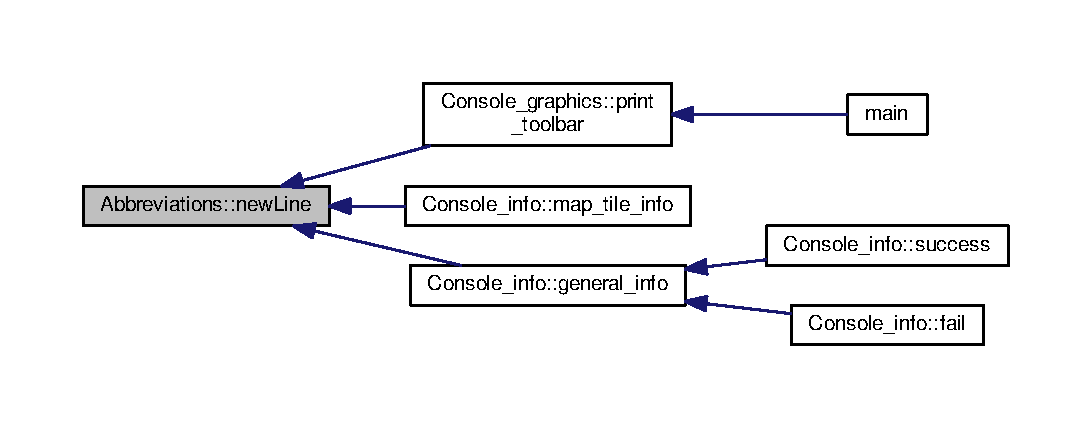
\includegraphics[width=350pt]{class_abbreviations_aa7ffcca4bdcae46e65910f19e5170e2c_icgraph}
\end{center}
\end{figure}


\hypertarget{class_abbreviations_a0d0f454b13d0d75b19d9c4febf015c59}{\index{Abbreviations@{Abbreviations}!set\-\_\-precision@{set\-\_\-precision}}
\index{set\-\_\-precision@{set\-\_\-precision}!Abbreviations@{Abbreviations}}
\subsubsection[{set\-\_\-precision}]{\setlength{\rightskip}{0pt plus 5cm}void Abbreviations\-::set\-\_\-precision (
\begin{DoxyParamCaption}
\item[{int}]{precision}
\end{DoxyParamCaption}
)}}\label{class_abbreviations_a0d0f454b13d0d75b19d9c4febf015c59}
\hypertarget{class_abbreviations_ad216697864106aa188a3209cc82ef4c2}{\index{Abbreviations@{Abbreviations}!skip\-\_\-page@{skip\-\_\-page}}
\index{skip\-\_\-page@{skip\-\_\-page}!Abbreviations@{Abbreviations}}
\subsubsection[{skip\-\_\-page}]{\setlength{\rightskip}{0pt plus 5cm}void Abbreviations\-::skip\-\_\-page (
\begin{DoxyParamCaption}
{}
\end{DoxyParamCaption}
)}}\label{class_abbreviations_ad216697864106aa188a3209cc82ef4c2}


Here is the caller graph for this function\-:\nopagebreak
\begin{figure}[H]
\begin{center}
\leavevmode
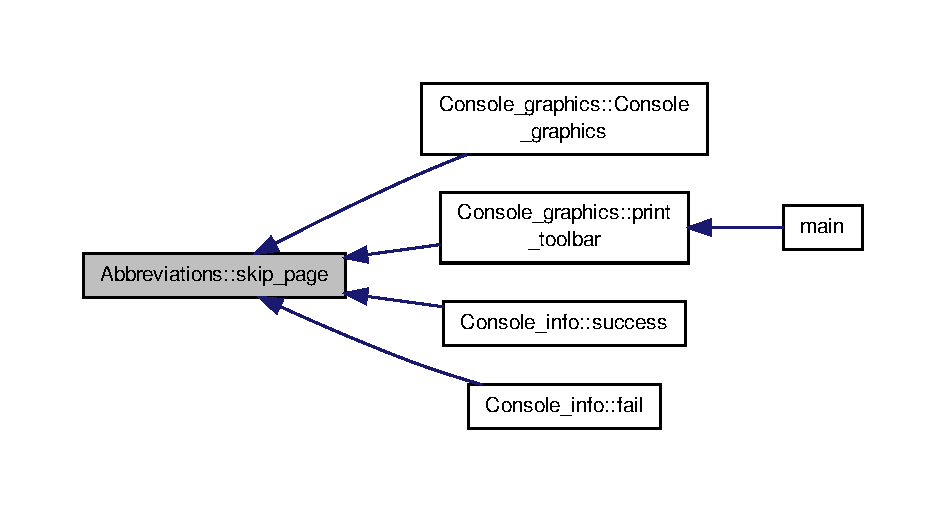
\includegraphics[width=350pt]{class_abbreviations_ad216697864106aa188a3209cc82ef4c2_icgraph}
\end{center}
\end{figure}


\hypertarget{class_abbreviations_a6f7cf8a3c4356bf2a8a5191e19b07d57}{\index{Abbreviations@{Abbreviations}!tab\-Left@{tab\-Left}}
\index{tab\-Left@{tab\-Left}!Abbreviations@{Abbreviations}}
\subsubsection[{tab\-Left}]{\setlength{\rightskip}{0pt plus 5cm}void Abbreviations\-::tab\-Left (
\begin{DoxyParamCaption}
\item[{int}]{tab}
\end{DoxyParamCaption}
)}}\label{class_abbreviations_a6f7cf8a3c4356bf2a8a5191e19b07d57}


The documentation for this class was generated from the following files\-:\begin{DoxyCompactItemize}
\item 
/home/baios/\-Cpp\-\_\-\-Projects/\-Cpp\-Ceid/include/backend/\hyperlink{_abbreviations_8h}{Abbreviations.\-h}\item 
/home/baios/\-Cpp\-\_\-\-Projects/\-Cpp\-Ceid/src/backend/\hyperlink{_abbreviations_8cpp}{Abbreviations.\-cpp}\end{DoxyCompactItemize}

\hypertarget{class_analysis_robot}{\section{Analysis\-Robot Class Reference}
\label{class_analysis_robot}\index{Analysis\-Robot@{Analysis\-Robot}}
}


{\ttfamily \#include $<$Analysis\-Robot.\-h$>$}



Inheritance diagram for Analysis\-Robot\-:\nopagebreak
\begin{figure}[H]
\begin{center}
\leavevmode
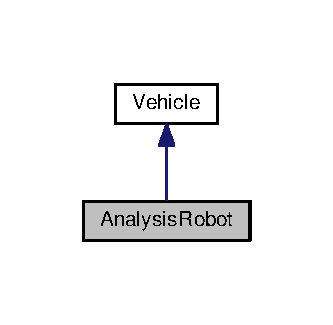
\includegraphics[width=160pt]{class_analysis_robot__inherit__graph}
\end{center}
\end{figure}


Collaboration diagram for Analysis\-Robot\-:\nopagebreak
\begin{figure}[H]
\begin{center}
\leavevmode
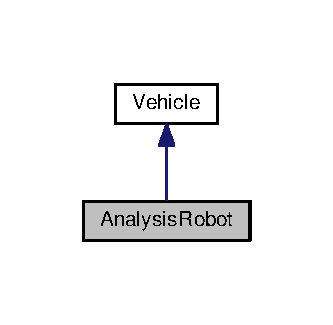
\includegraphics[width=160pt]{class_analysis_robot__coll__graph}
\end{center}
\end{figure}
\subsection*{Public Member Functions}
\begin{DoxyCompactItemize}
\item 
\hyperlink{class_analysis_robot_a4bc986573a8c243c3491e2c31099a50b}{Analysis\-Robot} (int id, const int width, const int height)
\item 
virtual void \hyperlink{class_analysis_robot_a496ce06a9eee3fcbb521dd6eb9ef7947}{operate} (\hyperlink{class_map}{Map} \&m)
\item 
float \hyperlink{class_analysis_robot_a054aeffeadbe44c99bff3ca9069d3f5d}{get\-\_\-total\-\_\-p} ()
\item 
float \hyperlink{class_analysis_robot_a4b673c341a4c706a99ad0df16b2ad1f6}{get\-\_\-total\-\_\-g} ()
\item 
float \hyperlink{class_analysis_robot_ab72c7c197faef7c9e30f502414a15b50}{get\-\_\-total\-\_\-i} ()
\item 
float \hyperlink{class_analysis_robot_a69ab14d80084ad9c5f0d7be077b04a65}{get\-\_\-total\-\_\-res\-\_\-picked} ()
\item 
virtual void \hyperlink{class_analysis_robot_a984f9a02843c487538dcb8029f15ce1f}{export\-\_\-info} (float \&p, float \&g, float \&i, float \&tot)
\item 
virtual void \hyperlink{class_analysis_robot_a090c8f17c57af7c3073905fa9bedbf2c}{export\-\_\-total\-\_\-info} (float \&tp, float \&tg, float \&ti, float \&total\-\_\-res)
\end{DoxyCompactItemize}
\subsection*{Public Attributes}
\begin{DoxyCompactItemize}
\item 
float \hyperlink{class_analysis_robot_a1cc3b0734f5e183c01aedf9fb563e9bb}{inventory} \mbox{[}3\mbox{]}
\item 
float \hyperlink{class_analysis_robot_a14ed4ba869e1dedc9100c1ce357b235d}{rem\-Load}
\end{DoxyCompactItemize}


\subsection{Constructor \& Destructor Documentation}
\hypertarget{class_analysis_robot_a4bc986573a8c243c3491e2c31099a50b}{\index{Analysis\-Robot@{Analysis\-Robot}!Analysis\-Robot@{Analysis\-Robot}}
\index{Analysis\-Robot@{Analysis\-Robot}!AnalysisRobot@{Analysis\-Robot}}
\subsubsection[{Analysis\-Robot}]{\setlength{\rightskip}{0pt plus 5cm}Analysis\-Robot\-::\-Analysis\-Robot (
\begin{DoxyParamCaption}
\item[{int}]{id, }
\item[{const int}]{width, }
\item[{const int}]{height}
\end{DoxyParamCaption}
)}}\label{class_analysis_robot_a4bc986573a8c243c3491e2c31099a50b}


Here is the call graph for this function\-:\nopagebreak
\begin{figure}[H]
\begin{center}
\leavevmode
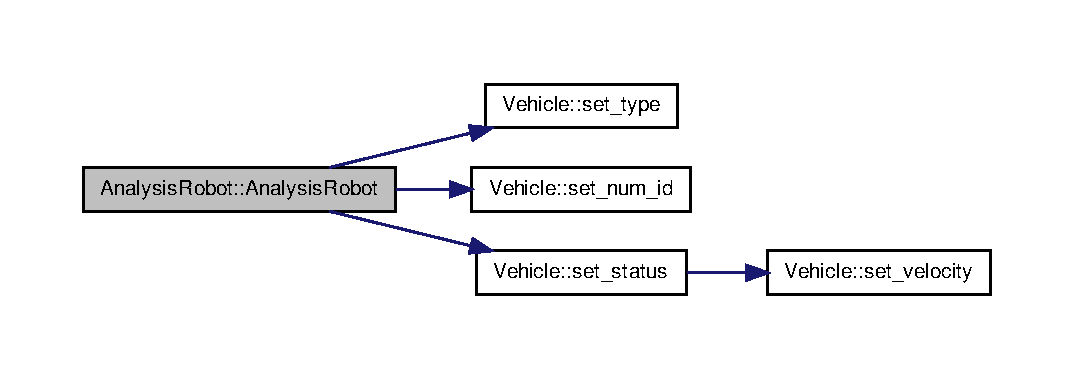
\includegraphics[width=350pt]{class_analysis_robot_a4bc986573a8c243c3491e2c31099a50b_cgraph}
\end{center}
\end{figure}




\subsection{Member Function Documentation}
\hypertarget{class_analysis_robot_a984f9a02843c487538dcb8029f15ce1f}{\index{Analysis\-Robot@{Analysis\-Robot}!export\-\_\-info@{export\-\_\-info}}
\index{export\-\_\-info@{export\-\_\-info}!AnalysisRobot@{Analysis\-Robot}}
\subsubsection[{export\-\_\-info}]{\setlength{\rightskip}{0pt plus 5cm}void Analysis\-Robot\-::export\-\_\-info (
\begin{DoxyParamCaption}
\item[{float \&}]{p, }
\item[{float \&}]{g, }
\item[{float \&}]{i, }
\item[{float \&}]{tot}
\end{DoxyParamCaption}
)\hspace{0.3cm}{\ttfamily [virtual]}}}\label{class_analysis_robot_a984f9a02843c487538dcb8029f15ce1f}


Reimplemented from \hyperlink{class_vehicle_a3e3cc666c76c42178e942363585ff1b7}{Vehicle}.

\hypertarget{class_analysis_robot_a090c8f17c57af7c3073905fa9bedbf2c}{\index{Analysis\-Robot@{Analysis\-Robot}!export\-\_\-total\-\_\-info@{export\-\_\-total\-\_\-info}}
\index{export\-\_\-total\-\_\-info@{export\-\_\-total\-\_\-info}!AnalysisRobot@{Analysis\-Robot}}
\subsubsection[{export\-\_\-total\-\_\-info}]{\setlength{\rightskip}{0pt plus 5cm}void Analysis\-Robot\-::export\-\_\-total\-\_\-info (
\begin{DoxyParamCaption}
\item[{float \&}]{tp, }
\item[{float \&}]{tg, }
\item[{float \&}]{ti, }
\item[{float \&}]{total\-\_\-res}
\end{DoxyParamCaption}
)\hspace{0.3cm}{\ttfamily [virtual]}}}\label{class_analysis_robot_a090c8f17c57af7c3073905fa9bedbf2c}


Reimplemented from \hyperlink{class_vehicle_ae2840b7627d758e5019a6fdd83a229a9}{Vehicle}.

\hypertarget{class_analysis_robot_a4b673c341a4c706a99ad0df16b2ad1f6}{\index{Analysis\-Robot@{Analysis\-Robot}!get\-\_\-total\-\_\-g@{get\-\_\-total\-\_\-g}}
\index{get\-\_\-total\-\_\-g@{get\-\_\-total\-\_\-g}!AnalysisRobot@{Analysis\-Robot}}
\subsubsection[{get\-\_\-total\-\_\-g}]{\setlength{\rightskip}{0pt plus 5cm}float Analysis\-Robot\-::get\-\_\-total\-\_\-g (
\begin{DoxyParamCaption}
{}
\end{DoxyParamCaption}
)}}\label{class_analysis_robot_a4b673c341a4c706a99ad0df16b2ad1f6}
\hypertarget{class_analysis_robot_ab72c7c197faef7c9e30f502414a15b50}{\index{Analysis\-Robot@{Analysis\-Robot}!get\-\_\-total\-\_\-i@{get\-\_\-total\-\_\-i}}
\index{get\-\_\-total\-\_\-i@{get\-\_\-total\-\_\-i}!AnalysisRobot@{Analysis\-Robot}}
\subsubsection[{get\-\_\-total\-\_\-i}]{\setlength{\rightskip}{0pt plus 5cm}float Analysis\-Robot\-::get\-\_\-total\-\_\-i (
\begin{DoxyParamCaption}
{}
\end{DoxyParamCaption}
)}}\label{class_analysis_robot_ab72c7c197faef7c9e30f502414a15b50}
\hypertarget{class_analysis_robot_a054aeffeadbe44c99bff3ca9069d3f5d}{\index{Analysis\-Robot@{Analysis\-Robot}!get\-\_\-total\-\_\-p@{get\-\_\-total\-\_\-p}}
\index{get\-\_\-total\-\_\-p@{get\-\_\-total\-\_\-p}!AnalysisRobot@{Analysis\-Robot}}
\subsubsection[{get\-\_\-total\-\_\-p}]{\setlength{\rightskip}{0pt plus 5cm}float Analysis\-Robot\-::get\-\_\-total\-\_\-p (
\begin{DoxyParamCaption}
{}
\end{DoxyParamCaption}
)}}\label{class_analysis_robot_a054aeffeadbe44c99bff3ca9069d3f5d}
\hypertarget{class_analysis_robot_a69ab14d80084ad9c5f0d7be077b04a65}{\index{Analysis\-Robot@{Analysis\-Robot}!get\-\_\-total\-\_\-res\-\_\-picked@{get\-\_\-total\-\_\-res\-\_\-picked}}
\index{get\-\_\-total\-\_\-res\-\_\-picked@{get\-\_\-total\-\_\-res\-\_\-picked}!AnalysisRobot@{Analysis\-Robot}}
\subsubsection[{get\-\_\-total\-\_\-res\-\_\-picked}]{\setlength{\rightskip}{0pt plus 5cm}float Analysis\-Robot\-::get\-\_\-total\-\_\-res\-\_\-picked (
\begin{DoxyParamCaption}
{}
\end{DoxyParamCaption}
)}}\label{class_analysis_robot_a69ab14d80084ad9c5f0d7be077b04a65}
\hypertarget{class_analysis_robot_a496ce06a9eee3fcbb521dd6eb9ef7947}{\index{Analysis\-Robot@{Analysis\-Robot}!operate@{operate}}
\index{operate@{operate}!AnalysisRobot@{Analysis\-Robot}}
\subsubsection[{operate}]{\setlength{\rightskip}{0pt plus 5cm}void Analysis\-Robot\-::operate (
\begin{DoxyParamCaption}
\item[{{\bf Map} \&}]{m}
\end{DoxyParamCaption}
)\hspace{0.3cm}{\ttfamily [virtual]}}}\label{class_analysis_robot_a496ce06a9eee3fcbb521dd6eb9ef7947}


Implements \hyperlink{class_vehicle_a6a0ed71ee9d4c569ee26961b213775db}{Vehicle}.



Here is the call graph for this function\-:\nopagebreak
\begin{figure}[H]
\begin{center}
\leavevmode
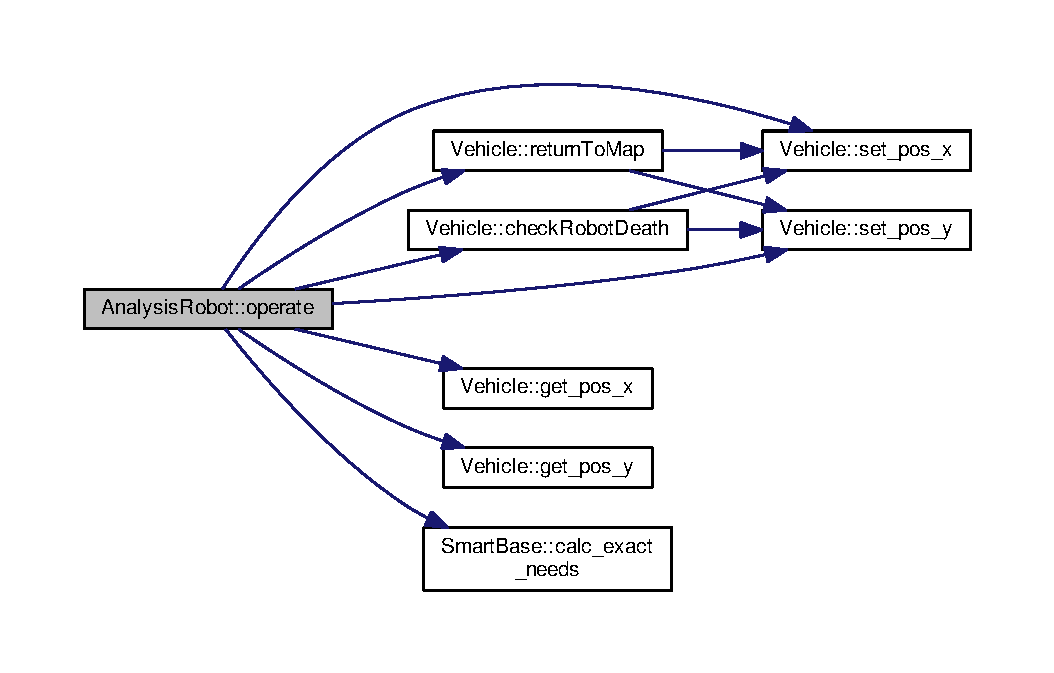
\includegraphics[width=350pt]{class_analysis_robot_a496ce06a9eee3fcbb521dd6eb9ef7947_cgraph}
\end{center}
\end{figure}




\subsection{Member Data Documentation}
\hypertarget{class_analysis_robot_a1cc3b0734f5e183c01aedf9fb563e9bb}{\index{Analysis\-Robot@{Analysis\-Robot}!inventory@{inventory}}
\index{inventory@{inventory}!AnalysisRobot@{Analysis\-Robot}}
\subsubsection[{inventory}]{\setlength{\rightskip}{0pt plus 5cm}float Analysis\-Robot\-::inventory\mbox{[}3\mbox{]}}}\label{class_analysis_robot_a1cc3b0734f5e183c01aedf9fb563e9bb}
\hypertarget{class_analysis_robot_a14ed4ba869e1dedc9100c1ce357b235d}{\index{Analysis\-Robot@{Analysis\-Robot}!rem\-Load@{rem\-Load}}
\index{rem\-Load@{rem\-Load}!AnalysisRobot@{Analysis\-Robot}}
\subsubsection[{rem\-Load}]{\setlength{\rightskip}{0pt plus 5cm}float Analysis\-Robot\-::rem\-Load}}\label{class_analysis_robot_a14ed4ba869e1dedc9100c1ce357b235d}


The documentation for this class was generated from the following files\-:\begin{DoxyCompactItemize}
\item 
/home/baios/\-Cpp\-\_\-\-Projects/\-Cpp\-Ceid/include/backend/\hyperlink{_analysis_robot_8h}{Analysis\-Robot.\-h}\item 
/home/baios/\-Cpp\-\_\-\-Projects/\-Cpp\-Ceid/src/backend/\hyperlink{_analysis_robot_8cpp}{Analysis\-Robot.\-cpp}\end{DoxyCompactItemize}

\hypertarget{class_console__graphics}{\section{Console\-\_\-graphics Class Reference}
\label{class_console__graphics}\index{Console\-\_\-graphics@{Console\-\_\-graphics}}
}


{\ttfamily \#include $<$Console\-\_\-graphics.\-h$>$}

\subsection*{Public Member Functions}
\begin{DoxyCompactItemize}
\item 
\hyperlink{class_console__graphics_a7dc8bfa26213dc3a53941b0612013f54}{Console\-\_\-graphics} (\hyperlink{class_map}{Map} \&m)
\item 
bool \hyperlink{class_console__graphics_a521fbb62bb9b5be454b903bf67499bf8}{choice} ()
\item 
void \hyperlink{class_console__graphics_a4b20f4a9ea5fad4820ddd1fe2232affc}{print\-\_\-toolbar} ()
\end{DoxyCompactItemize}


\subsection{Constructor \& Destructor Documentation}
\hypertarget{class_console__graphics_a7dc8bfa26213dc3a53941b0612013f54}{\index{Console\-\_\-graphics@{Console\-\_\-graphics}!Console\-\_\-graphics@{Console\-\_\-graphics}}
\index{Console\-\_\-graphics@{Console\-\_\-graphics}!Console_graphics@{Console\-\_\-graphics}}
\subsubsection[{Console\-\_\-graphics}]{\setlength{\rightskip}{0pt plus 5cm}Console\-\_\-graphics\-::\-Console\-\_\-graphics (
\begin{DoxyParamCaption}
\item[{{\bf Map} \&}]{m}
\end{DoxyParamCaption}
)}}\label{class_console__graphics_a7dc8bfa26213dc3a53941b0612013f54}


Here is the call graph for this function\-:
\nopagebreak
\begin{figure}[H]
\begin{center}
\leavevmode
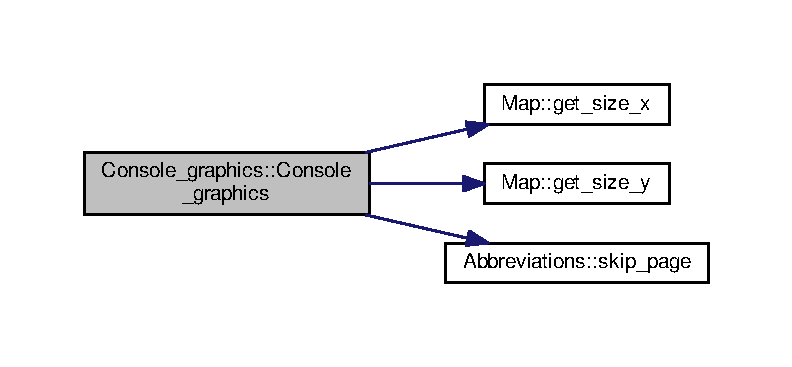
\includegraphics[width=350pt]{class_console__graphics_a7dc8bfa26213dc3a53941b0612013f54_cgraph}
\end{center}
\end{figure}




\subsection{Member Function Documentation}
\hypertarget{class_console__graphics_a521fbb62bb9b5be454b903bf67499bf8}{\index{Console\-\_\-graphics@{Console\-\_\-graphics}!choice@{choice}}
\index{choice@{choice}!Console_graphics@{Console\-\_\-graphics}}
\subsubsection[{choice}]{\setlength{\rightskip}{0pt plus 5cm}bool Console\-\_\-graphics\-::choice (
\begin{DoxyParamCaption}
{}
\end{DoxyParamCaption}
)}}\label{class_console__graphics_a521fbb62bb9b5be454b903bf67499bf8}
\hypertarget{class_console__graphics_a4b20f4a9ea5fad4820ddd1fe2232affc}{\index{Console\-\_\-graphics@{Console\-\_\-graphics}!print\-\_\-toolbar@{print\-\_\-toolbar}}
\index{print\-\_\-toolbar@{print\-\_\-toolbar}!Console_graphics@{Console\-\_\-graphics}}
\subsubsection[{print\-\_\-toolbar}]{\setlength{\rightskip}{0pt plus 5cm}void Console\-\_\-graphics\-::print\-\_\-toolbar (
\begin{DoxyParamCaption}
{}
\end{DoxyParamCaption}
)}}\label{class_console__graphics_a4b20f4a9ea5fad4820ddd1fe2232affc}


Here is the call graph for this function\-:
\nopagebreak
\begin{figure}[H]
\begin{center}
\leavevmode
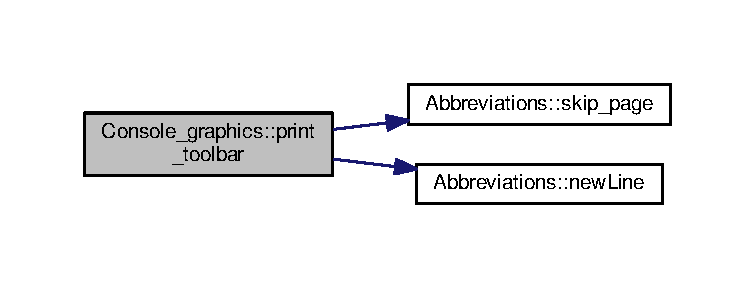
\includegraphics[width=350pt]{class_console__graphics_a4b20f4a9ea5fad4820ddd1fe2232affc_cgraph}
\end{center}
\end{figure}




Here is the caller graph for this function\-:
\nopagebreak
\begin{figure}[H]
\begin{center}
\leavevmode
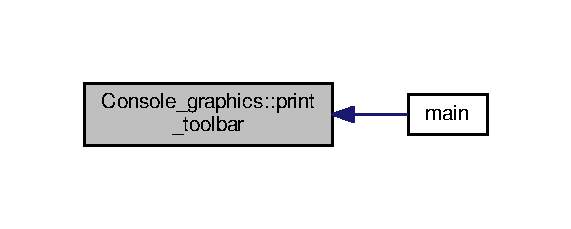
\includegraphics[width=274pt]{class_console__graphics_a4b20f4a9ea5fad4820ddd1fe2232affc_icgraph}
\end{center}
\end{figure}




The documentation for this class was generated from the following files\-:\begin{DoxyCompactItemize}
\item 
/home/baios/\-Desktop/robsim/\-Rob\-Sim/include/frontend/\-Console/\hyperlink{_console__graphics_8h}{Console\-\_\-graphics.\-h}\item 
/home/baios/\-Desktop/robsim/\-Rob\-Sim/src/frontend/\-Console/\hyperlink{_console__graphics_8cpp}{Console\-\_\-graphics.\-cpp}\end{DoxyCompactItemize}

\hypertarget{class_console__info}{\section{Console\-\_\-info Class Reference}
\label{class_console__info}\index{Console\-\_\-info@{Console\-\_\-info}}
}


{\ttfamily \#include $<$Console\-\_\-info.\-h$>$}

\subsection*{Public Member Functions}
\begin{DoxyCompactItemize}
\item 
\hyperlink{class_console__info_aa3e98bbb783ce050426ebd5ee8ce17e8}{Console\-\_\-info} (\hyperlink{class_map}{Map} m)
\item 
void \hyperlink{class_console__info_adf9b1b99dbecf11b50862618f0b5e2ad}{robot\-Moved\-To} (char type, int id, int x, int y)
\item 
void \hyperlink{class_console__info_a050bd493a7c149a9c70680170d19595a}{map\-\_\-tile\-\_\-info} (int x, int y)
\item 
void \hyperlink{class_console__info_ac1231a972e38ec0f7142a20641cb7663}{robot\-\_\-info} (int id)
\item 
void \hyperlink{class_console__info_a2ade25393df6aab1fa014363b002b372}{robot\-\_\-info} (\hyperlink{_robot__management_8h_a4d3943ddea65db7163a58e6c7e8df95a}{uint} x, \hyperlink{_robot__management_8h_a4d3943ddea65db7163a58e6c7e8df95a}{uint} y)
\item 
void \hyperlink{class_console__info_a261e6ecc446e58253dcf2df814c62d61}{analysis\-\_\-info} (int id)
\item 
void \hyperlink{class_console__info_a10e4c45fbe8b8fab856b15fc6283a191}{rescue\-\_\-info} (int id)
\item 
void \hyperlink{class_console__info_ae39b4f0b5455c9c554942119b0f89060}{research\-\_\-info} (int id)
\item 
void \hyperlink{class_console__info_a2984a90ee439b84e463f763c42df0ff8}{took\-\_\-damage} (int damage)
\item 
void \hyperlink{class_console__info_ac75c6db03c6bda9b33de56696b6a18d4}{success} ()
\item 
void \hyperlink{class_console__info_a29875cecf1aa23eceac4bb46d4df7598}{fail} ()
\item 
void \hyperlink{class_console__info_afa4567c4eeccc5ea70fe33a0bcfef4fd}{general\-\_\-info} ()
\end{DoxyCompactItemize}


\subsection{Constructor \& Destructor Documentation}
\hypertarget{class_console__info_aa3e98bbb783ce050426ebd5ee8ce17e8}{\index{Console\-\_\-info@{Console\-\_\-info}!Console\-\_\-info@{Console\-\_\-info}}
\index{Console\-\_\-info@{Console\-\_\-info}!Console_info@{Console\-\_\-info}}
\subsubsection[{Console\-\_\-info}]{\setlength{\rightskip}{0pt plus 5cm}Console\-\_\-info\-::\-Console\-\_\-info (
\begin{DoxyParamCaption}
\item[{{\bf Map}}]{m}
\end{DoxyParamCaption}
)}}\label{class_console__info_aa3e98bbb783ce050426ebd5ee8ce17e8}


\subsection{Member Function Documentation}
\hypertarget{class_console__info_a261e6ecc446e58253dcf2df814c62d61}{\index{Console\-\_\-info@{Console\-\_\-info}!analysis\-\_\-info@{analysis\-\_\-info}}
\index{analysis\-\_\-info@{analysis\-\_\-info}!Console_info@{Console\-\_\-info}}
\subsubsection[{analysis\-\_\-info}]{\setlength{\rightskip}{0pt plus 5cm}void Console\-\_\-info\-::analysis\-\_\-info (
\begin{DoxyParamCaption}
\item[{int}]{id}
\end{DoxyParamCaption}
)}}\label{class_console__info_a261e6ecc446e58253dcf2df814c62d61}
\hypertarget{class_console__info_a29875cecf1aa23eceac4bb46d4df7598}{\index{Console\-\_\-info@{Console\-\_\-info}!fail@{fail}}
\index{fail@{fail}!Console_info@{Console\-\_\-info}}
\subsubsection[{fail}]{\setlength{\rightskip}{0pt plus 5cm}void Console\-\_\-info\-::fail (
\begin{DoxyParamCaption}
{}
\end{DoxyParamCaption}
)}}\label{class_console__info_a29875cecf1aa23eceac4bb46d4df7598}


Here is the call graph for this function\-:
\nopagebreak
\begin{figure}[H]
\begin{center}
\leavevmode
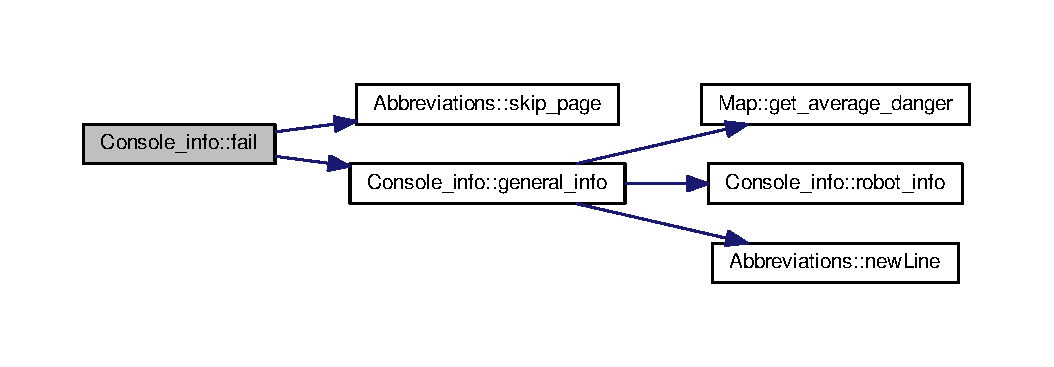
\includegraphics[width=350pt]{class_console__info_a29875cecf1aa23eceac4bb46d4df7598_cgraph}
\end{center}
\end{figure}


\hypertarget{class_console__info_afa4567c4eeccc5ea70fe33a0bcfef4fd}{\index{Console\-\_\-info@{Console\-\_\-info}!general\-\_\-info@{general\-\_\-info}}
\index{general\-\_\-info@{general\-\_\-info}!Console_info@{Console\-\_\-info}}
\subsubsection[{general\-\_\-info}]{\setlength{\rightskip}{0pt plus 5cm}void Console\-\_\-info\-::general\-\_\-info (
\begin{DoxyParamCaption}
{}
\end{DoxyParamCaption}
)}}\label{class_console__info_afa4567c4eeccc5ea70fe33a0bcfef4fd}


Here is the call graph for this function\-:
\nopagebreak
\begin{figure}[H]
\begin{center}
\leavevmode
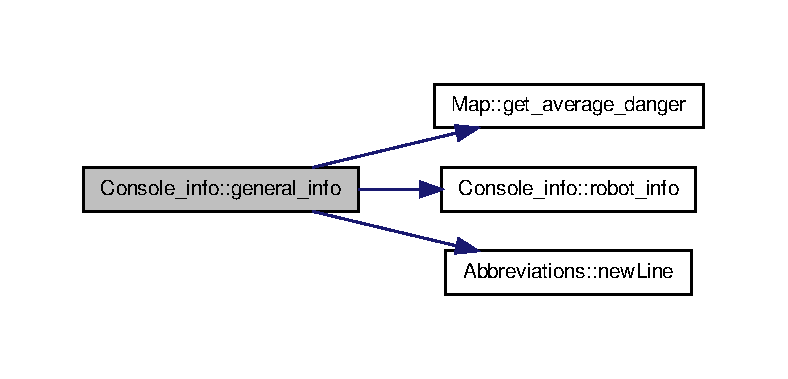
\includegraphics[width=350pt]{class_console__info_afa4567c4eeccc5ea70fe33a0bcfef4fd_cgraph}
\end{center}
\end{figure}




Here is the caller graph for this function\-:
\nopagebreak
\begin{figure}[H]
\begin{center}
\leavevmode
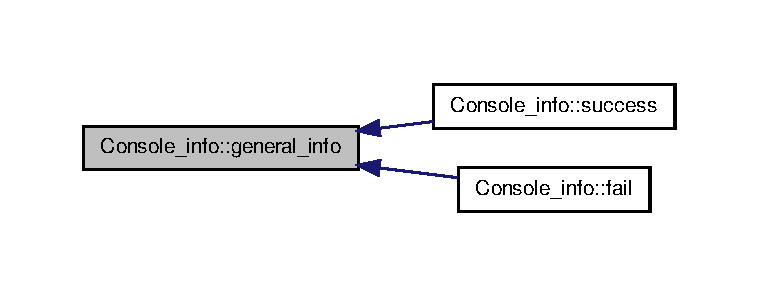
\includegraphics[width=350pt]{class_console__info_afa4567c4eeccc5ea70fe33a0bcfef4fd_icgraph}
\end{center}
\end{figure}


\hypertarget{class_console__info_a050bd493a7c149a9c70680170d19595a}{\index{Console\-\_\-info@{Console\-\_\-info}!map\-\_\-tile\-\_\-info@{map\-\_\-tile\-\_\-info}}
\index{map\-\_\-tile\-\_\-info@{map\-\_\-tile\-\_\-info}!Console_info@{Console\-\_\-info}}
\subsubsection[{map\-\_\-tile\-\_\-info}]{\setlength{\rightskip}{0pt plus 5cm}void Console\-\_\-info\-::map\-\_\-tile\-\_\-info (
\begin{DoxyParamCaption}
\item[{int}]{x, }
\item[{int}]{y}
\end{DoxyParamCaption}
)}}\label{class_console__info_a050bd493a7c149a9c70680170d19595a}


Here is the call graph for this function\-:
\nopagebreak
\begin{figure}[H]
\begin{center}
\leavevmode
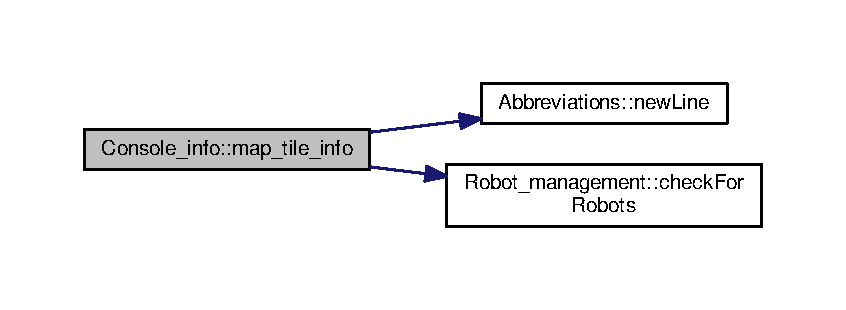
\includegraphics[width=350pt]{class_console__info_a050bd493a7c149a9c70680170d19595a_cgraph}
\end{center}
\end{figure}


\hypertarget{class_console__info_a10e4c45fbe8b8fab856b15fc6283a191}{\index{Console\-\_\-info@{Console\-\_\-info}!rescue\-\_\-info@{rescue\-\_\-info}}
\index{rescue\-\_\-info@{rescue\-\_\-info}!Console_info@{Console\-\_\-info}}
\subsubsection[{rescue\-\_\-info}]{\setlength{\rightskip}{0pt plus 5cm}void Console\-\_\-info\-::rescue\-\_\-info (
\begin{DoxyParamCaption}
\item[{int}]{id}
\end{DoxyParamCaption}
)}}\label{class_console__info_a10e4c45fbe8b8fab856b15fc6283a191}
\hypertarget{class_console__info_ae39b4f0b5455c9c554942119b0f89060}{\index{Console\-\_\-info@{Console\-\_\-info}!research\-\_\-info@{research\-\_\-info}}
\index{research\-\_\-info@{research\-\_\-info}!Console_info@{Console\-\_\-info}}
\subsubsection[{research\-\_\-info}]{\setlength{\rightskip}{0pt plus 5cm}void Console\-\_\-info\-::research\-\_\-info (
\begin{DoxyParamCaption}
\item[{int}]{id}
\end{DoxyParamCaption}
)}}\label{class_console__info_ae39b4f0b5455c9c554942119b0f89060}
\hypertarget{class_console__info_ac1231a972e38ec0f7142a20641cb7663}{\index{Console\-\_\-info@{Console\-\_\-info}!robot\-\_\-info@{robot\-\_\-info}}
\index{robot\-\_\-info@{robot\-\_\-info}!Console_info@{Console\-\_\-info}}
\subsubsection[{robot\-\_\-info}]{\setlength{\rightskip}{0pt plus 5cm}void Console\-\_\-info\-::robot\-\_\-info (
\begin{DoxyParamCaption}
\item[{int}]{id}
\end{DoxyParamCaption}
)}}\label{class_console__info_ac1231a972e38ec0f7142a20641cb7663}


Here is the caller graph for this function\-:
\nopagebreak
\begin{figure}[H]
\begin{center}
\leavevmode
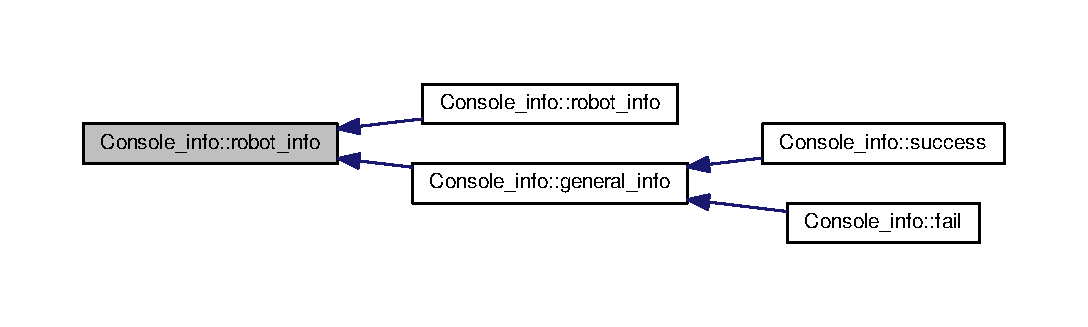
\includegraphics[width=350pt]{class_console__info_ac1231a972e38ec0f7142a20641cb7663_icgraph}
\end{center}
\end{figure}


\hypertarget{class_console__info_a2ade25393df6aab1fa014363b002b372}{\index{Console\-\_\-info@{Console\-\_\-info}!robot\-\_\-info@{robot\-\_\-info}}
\index{robot\-\_\-info@{robot\-\_\-info}!Console_info@{Console\-\_\-info}}
\subsubsection[{robot\-\_\-info}]{\setlength{\rightskip}{0pt plus 5cm}void Console\-\_\-info\-::robot\-\_\-info (
\begin{DoxyParamCaption}
\item[{{\bf uint}}]{x, }
\item[{{\bf uint}}]{y}
\end{DoxyParamCaption}
)}}\label{class_console__info_a2ade25393df6aab1fa014363b002b372}


Here is the call graph for this function\-:
\nopagebreak
\begin{figure}[H]
\begin{center}
\leavevmode
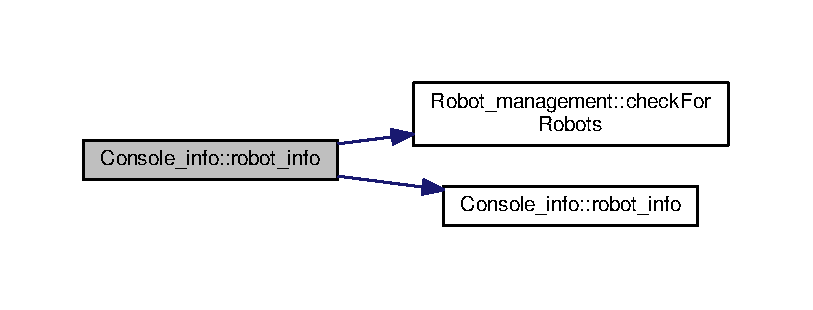
\includegraphics[width=350pt]{class_console__info_a2ade25393df6aab1fa014363b002b372_cgraph}
\end{center}
\end{figure}


\hypertarget{class_console__info_adf9b1b99dbecf11b50862618f0b5e2ad}{\index{Console\-\_\-info@{Console\-\_\-info}!robot\-Moved\-To@{robot\-Moved\-To}}
\index{robot\-Moved\-To@{robot\-Moved\-To}!Console_info@{Console\-\_\-info}}
\subsubsection[{robot\-Moved\-To}]{\setlength{\rightskip}{0pt plus 5cm}void Console\-\_\-info\-::robot\-Moved\-To (
\begin{DoxyParamCaption}
\item[{char}]{type, }
\item[{int}]{id, }
\item[{int}]{x, }
\item[{int}]{y}
\end{DoxyParamCaption}
)}}\label{class_console__info_adf9b1b99dbecf11b50862618f0b5e2ad}
\hypertarget{class_console__info_ac75c6db03c6bda9b33de56696b6a18d4}{\index{Console\-\_\-info@{Console\-\_\-info}!success@{success}}
\index{success@{success}!Console_info@{Console\-\_\-info}}
\subsubsection[{success}]{\setlength{\rightskip}{0pt plus 5cm}void Console\-\_\-info\-::success (
\begin{DoxyParamCaption}
{}
\end{DoxyParamCaption}
)}}\label{class_console__info_ac75c6db03c6bda9b33de56696b6a18d4}


Here is the call graph for this function\-:
\nopagebreak
\begin{figure}[H]
\begin{center}
\leavevmode
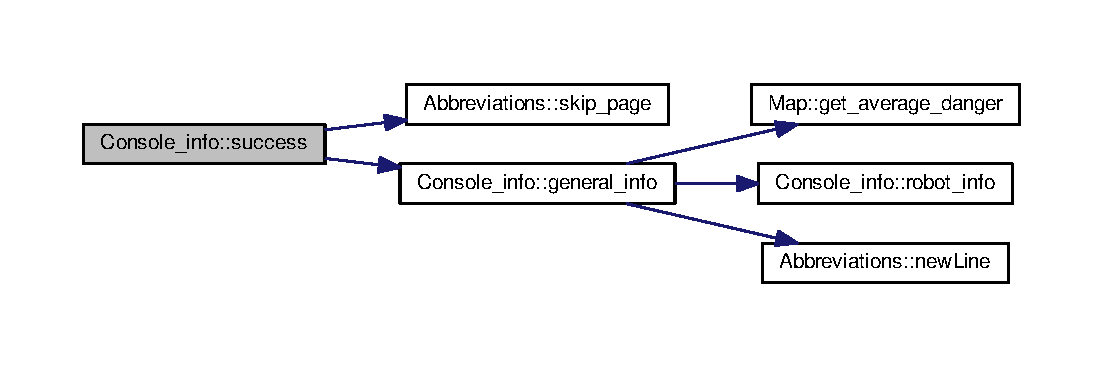
\includegraphics[width=350pt]{class_console__info_ac75c6db03c6bda9b33de56696b6a18d4_cgraph}
\end{center}
\end{figure}


\hypertarget{class_console__info_a2984a90ee439b84e463f763c42df0ff8}{\index{Console\-\_\-info@{Console\-\_\-info}!took\-\_\-damage@{took\-\_\-damage}}
\index{took\-\_\-damage@{took\-\_\-damage}!Console_info@{Console\-\_\-info}}
\subsubsection[{took\-\_\-damage}]{\setlength{\rightskip}{0pt plus 5cm}void Console\-\_\-info\-::took\-\_\-damage (
\begin{DoxyParamCaption}
\item[{int}]{damage}
\end{DoxyParamCaption}
)}}\label{class_console__info_a2984a90ee439b84e463f763c42df0ff8}


The documentation for this class was generated from the following files\-:\begin{DoxyCompactItemize}
\item 
/home/baios/\-Desktop/robsim/\-Rob\-Sim/include/frontend/\-Console/\hyperlink{_console__info_8h}{Console\-\_\-info.\-h}\item 
/home/baios/\-Desktop/robsim/\-Rob\-Sim/src/frontend/\-Console/\hyperlink{_console__info_8cpp}{Console\-\_\-info.\-cpp}\end{DoxyCompactItemize}

\hypertarget{class_gui}{\section{Gui Class Reference}
\label{class_gui}\index{Gui@{Gui}}
}


{\ttfamily \#include $<$Gui.\-h$>$}

\subsection*{Static Public Member Functions}
\begin{DoxyCompactItemize}
\item 
static void \hyperlink{class_gui_aa6ed2f385b49764852f9bb09ed9198ff}{init} (int argc, char $\ast$$\ast$\&argv, \hyperlink{class_map}{Map} m)
\end{DoxyCompactItemize}


\subsection{Member Function Documentation}
\hypertarget{class_gui_aa6ed2f385b49764852f9bb09ed9198ff}{\index{Gui@{Gui}!init@{init}}
\index{init@{init}!Gui@{Gui}}
\subsubsection[{init}]{\setlength{\rightskip}{0pt plus 5cm}void Gui\-::init (
\begin{DoxyParamCaption}
\item[{int}]{argc, }
\item[{char $\ast$$\ast$\&}]{argv, }
\item[{{\bf Map}}]{m}
\end{DoxyParamCaption}
)\hspace{0.3cm}{\ttfamily [static]}}}\label{class_gui_aa6ed2f385b49764852f9bb09ed9198ff}


Here is the call graph for this function\-:\nopagebreak
\begin{figure}[H]
\begin{center}
\leavevmode
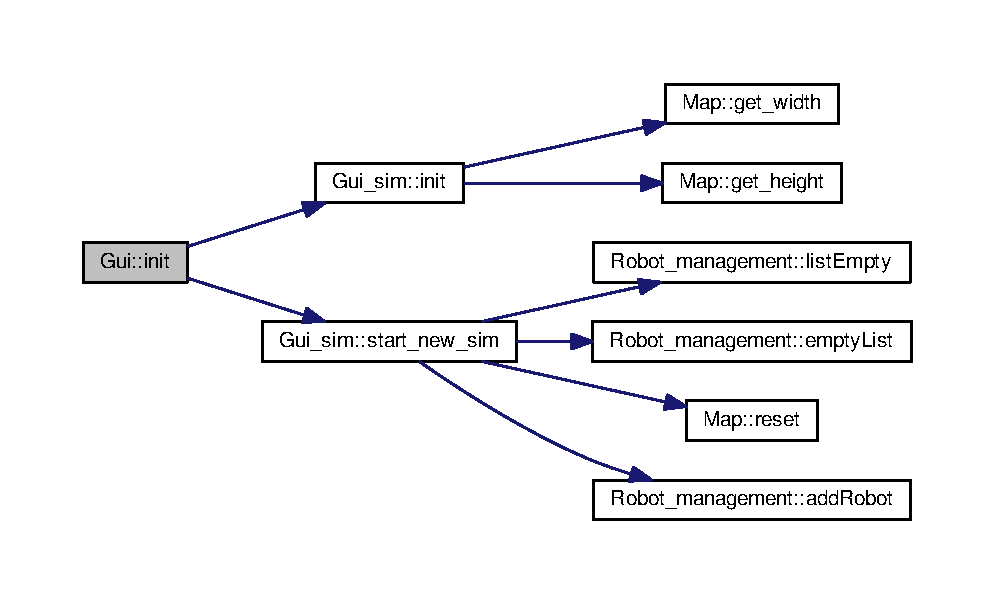
\includegraphics[width=350pt]{class_gui_aa6ed2f385b49764852f9bb09ed9198ff_cgraph}
\end{center}
\end{figure}




Here is the caller graph for this function\-:\nopagebreak
\begin{figure}[H]
\begin{center}
\leavevmode
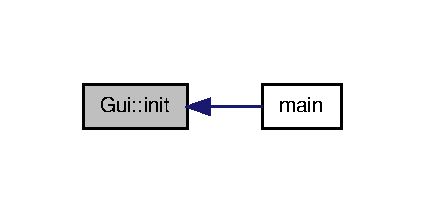
\includegraphics[width=204pt]{class_gui_aa6ed2f385b49764852f9bb09ed9198ff_icgraph}
\end{center}
\end{figure}




The documentation for this class was generated from the following files\-:\begin{DoxyCompactItemize}
\item 
/home/baios/\-Cpp\-\_\-\-Projects/\-Cpp\-Ceid/include/frontend/\-Gui/\hyperlink{_gui_8h}{Gui.\-h}\item 
/home/baios/\-Cpp\-\_\-\-Projects/\-Cpp\-Ceid/src/frontend/\-Gui/\hyperlink{_gui_8cpp}{Gui.\-cpp}\end{DoxyCompactItemize}

\hypertarget{class_gui__menus}{\section{Gui\-\_\-menus Class Reference}
\label{class_gui__menus}\index{Gui\-\_\-menus@{Gui\-\_\-menus}}
}


{\ttfamily \#include $<$Gui\-\_\-menus.\-h$>$}

\subsection*{Public Member Functions}
\begin{DoxyCompactItemize}
\item 
void \hyperlink{class_gui__menus_a9a6a464bbe50b7895ce2f09f09d7c752}{controls} (\hyperlink{_gui_8h_a199ee0f48afbd5920bf30972f7a381dc}{vec3f} C\-A\-M\-E\-R\-A\-\_\-\-P\-O\-S\-I\-T\-I\-O\-N)
\item 
void \hyperlink{class_gui__menus_a36b5bf60d6fb755a34ab7acb100ffac6}{round\-\_\-info} (int id, int w, int h)
\item 
void \hyperlink{class_gui__menus_a0380d9b643007661b1f9d80fb6e97c23}{base\-\_\-info} (\hyperlink{class_map}{Map} m)
\end{DoxyCompactItemize}


\subsection{Member Function Documentation}
\hypertarget{class_gui__menus_a0380d9b643007661b1f9d80fb6e97c23}{\index{Gui\-\_\-menus@{Gui\-\_\-menus}!base\-\_\-info@{base\-\_\-info}}
\index{base\-\_\-info@{base\-\_\-info}!Gui_menus@{Gui\-\_\-menus}}
\subsubsection[{base\-\_\-info}]{\setlength{\rightskip}{0pt plus 5cm}void Gui\-\_\-menus\-::base\-\_\-info (
\begin{DoxyParamCaption}
\item[{{\bf Map}}]{m}
\end{DoxyParamCaption}
)}}\label{class_gui__menus_a0380d9b643007661b1f9d80fb6e97c23}


Here is the call graph for this function\-:\nopagebreak
\begin{figure}[H]
\begin{center}
\leavevmode
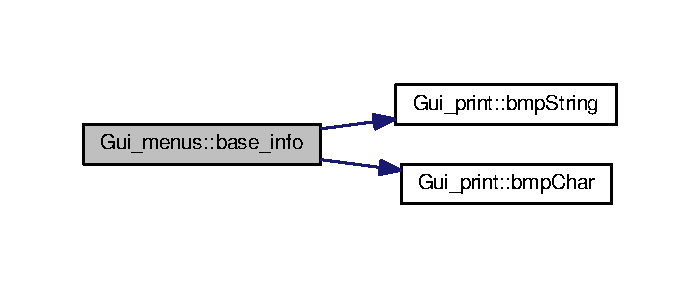
\includegraphics[width=336pt]{class_gui__menus_a0380d9b643007661b1f9d80fb6e97c23_cgraph}
\end{center}
\end{figure}




Here is the caller graph for this function\-:\nopagebreak
\begin{figure}[H]
\begin{center}
\leavevmode
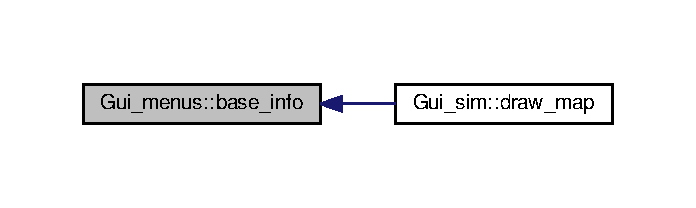
\includegraphics[width=334pt]{class_gui__menus_a0380d9b643007661b1f9d80fb6e97c23_icgraph}
\end{center}
\end{figure}


\hypertarget{class_gui__menus_a9a6a464bbe50b7895ce2f09f09d7c752}{\index{Gui\-\_\-menus@{Gui\-\_\-menus}!controls@{controls}}
\index{controls@{controls}!Gui_menus@{Gui\-\_\-menus}}
\subsubsection[{controls}]{\setlength{\rightskip}{0pt plus 5cm}void Gui\-\_\-menus\-::controls (
\begin{DoxyParamCaption}
\item[{{\bf vec3f}}]{C\-A\-M\-E\-R\-A\-\_\-\-P\-O\-S\-I\-T\-I\-O\-N}
\end{DoxyParamCaption}
)}}\label{class_gui__menus_a9a6a464bbe50b7895ce2f09f09d7c752}


Here is the call graph for this function\-:\nopagebreak
\begin{figure}[H]
\begin{center}
\leavevmode
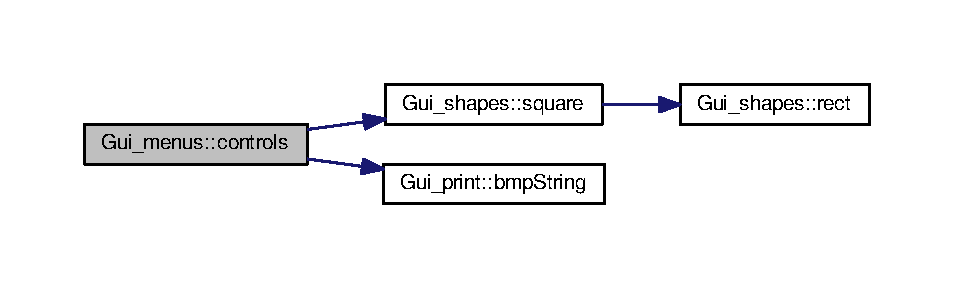
\includegraphics[width=350pt]{class_gui__menus_a9a6a464bbe50b7895ce2f09f09d7c752_cgraph}
\end{center}
\end{figure}


\hypertarget{class_gui__menus_a36b5bf60d6fb755a34ab7acb100ffac6}{\index{Gui\-\_\-menus@{Gui\-\_\-menus}!round\-\_\-info@{round\-\_\-info}}
\index{round\-\_\-info@{round\-\_\-info}!Gui_menus@{Gui\-\_\-menus}}
\subsubsection[{round\-\_\-info}]{\setlength{\rightskip}{0pt plus 5cm}void Gui\-\_\-menus\-::round\-\_\-info (
\begin{DoxyParamCaption}
\item[{int}]{id, }
\item[{int}]{w, }
\item[{int}]{h}
\end{DoxyParamCaption}
)}}\label{class_gui__menus_a36b5bf60d6fb755a34ab7acb100ffac6}


Here is the call graph for this function\-:\nopagebreak
\begin{figure}[H]
\begin{center}
\leavevmode
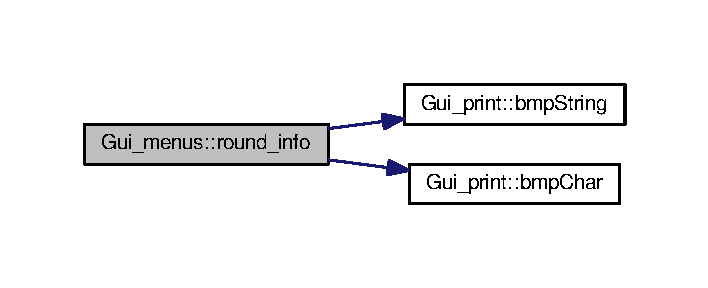
\includegraphics[width=340pt]{class_gui__menus_a36b5bf60d6fb755a34ab7acb100ffac6_cgraph}
\end{center}
\end{figure}




Here is the caller graph for this function\-:\nopagebreak
\begin{figure}[H]
\begin{center}
\leavevmode
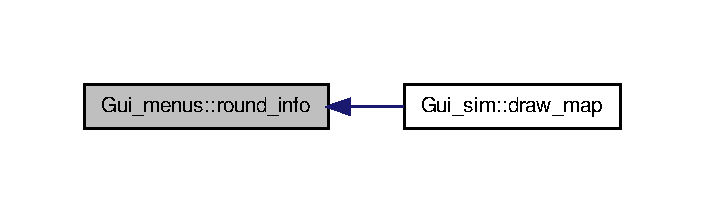
\includegraphics[width=338pt]{class_gui__menus_a36b5bf60d6fb755a34ab7acb100ffac6_icgraph}
\end{center}
\end{figure}




The documentation for this class was generated from the following files\-:\begin{DoxyCompactItemize}
\item 
/home/baios/\-Cpp\-\_\-\-Projects/\-Cpp\-Ceid/include/frontend/\-Gui/\hyperlink{_gui__menus_8h}{Gui\-\_\-menus.\-h}\item 
/home/baios/\-Cpp\-\_\-\-Projects/\-Cpp\-Ceid/src/frontend/\-Gui/\hyperlink{_gui__menus_8cpp}{Gui\-\_\-menus.\-cpp}\end{DoxyCompactItemize}

\hypertarget{class_gui__print}{\section{Gui\-\_\-print Class Reference}
\label{class_gui__print}\index{Gui\-\_\-print@{Gui\-\_\-print}}
}


{\ttfamily \#include $<$Gui\-\_\-print.\-h$>$}

\subsection*{Public Member Functions}
\begin{DoxyCompactItemize}
\item 
void \hyperlink{class_gui__print_a531bb6aa6c53e440b291f3bd62cd7711}{bmp\-String} (\hyperlink{class_gui__vector3f}{Gui\-\_\-vector3f} position, std\-::string str, void $\ast$font, \hyperlink{class_gui__vector3f}{Gui\-\_\-vector3f} Colour\-R\-G\-B)
\item 
void \hyperlink{class_gui__print_aa7f1ef73b3fa497738ec378bcf447fed}{bmp\-Char} (\hyperlink{class_gui__vector3f}{Gui\-\_\-vector3f} position, char ch, void $\ast$font, \hyperlink{class_gui__vector3f}{Gui\-\_\-vector3f} Colour\-R\-G\-B)
\end{DoxyCompactItemize}


\subsection{Member Function Documentation}
\hypertarget{class_gui__print_aa7f1ef73b3fa497738ec378bcf447fed}{\index{Gui\-\_\-print@{Gui\-\_\-print}!bmp\-Char@{bmp\-Char}}
\index{bmp\-Char@{bmp\-Char}!Gui_print@{Gui\-\_\-print}}
\subsubsection[{bmp\-Char}]{\setlength{\rightskip}{0pt plus 5cm}void Gui\-\_\-print\-::bmp\-Char (
\begin{DoxyParamCaption}
\item[{{\bf Gui\-\_\-vector3f}}]{position, }
\item[{char}]{ch, }
\item[{void $\ast$}]{font, }
\item[{{\bf Gui\-\_\-vector3f}}]{Colour\-R\-G\-B}
\end{DoxyParamCaption}
)}}\label{class_gui__print_aa7f1ef73b3fa497738ec378bcf447fed}


Here is the caller graph for this function\-:\nopagebreak
\begin{figure}[H]
\begin{center}
\leavevmode
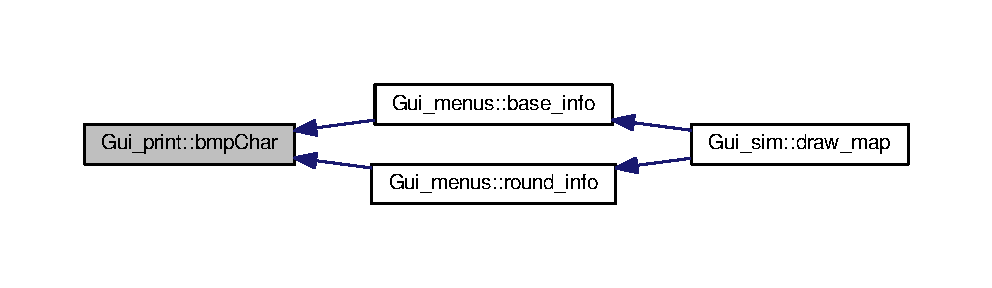
\includegraphics[width=350pt]{class_gui__print_aa7f1ef73b3fa497738ec378bcf447fed_icgraph}
\end{center}
\end{figure}


\hypertarget{class_gui__print_a531bb6aa6c53e440b291f3bd62cd7711}{\index{Gui\-\_\-print@{Gui\-\_\-print}!bmp\-String@{bmp\-String}}
\index{bmp\-String@{bmp\-String}!Gui_print@{Gui\-\_\-print}}
\subsubsection[{bmp\-String}]{\setlength{\rightskip}{0pt plus 5cm}void Gui\-\_\-print\-::bmp\-String (
\begin{DoxyParamCaption}
\item[{{\bf Gui\-\_\-vector3f}}]{position, }
\item[{std\-::string}]{str, }
\item[{void $\ast$}]{font, }
\item[{{\bf Gui\-\_\-vector3f}}]{Colour\-R\-G\-B}
\end{DoxyParamCaption}
)}}\label{class_gui__print_a531bb6aa6c53e440b291f3bd62cd7711}


Here is the caller graph for this function\-:\nopagebreak
\begin{figure}[H]
\begin{center}
\leavevmode
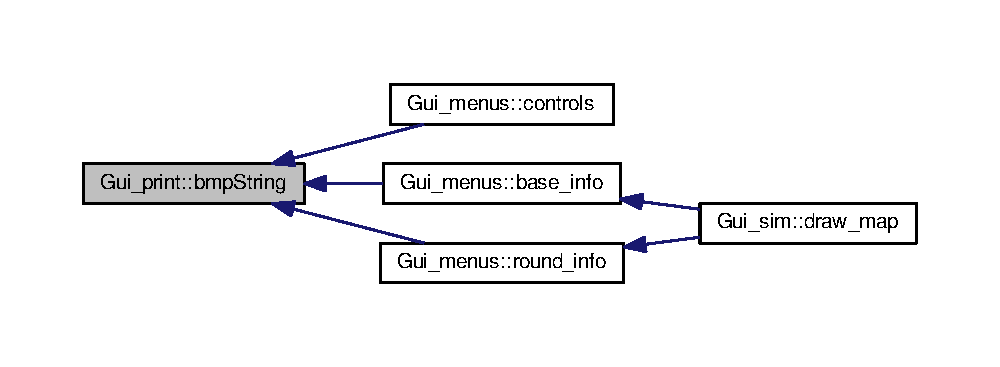
\includegraphics[width=350pt]{class_gui__print_a531bb6aa6c53e440b291f3bd62cd7711_icgraph}
\end{center}
\end{figure}




The documentation for this class was generated from the following files\-:\begin{DoxyCompactItemize}
\item 
/home/baios/\-Cpp\-\_\-\-Projects/\-Cpp\-Ceid/include/frontend/\-Gui/\hyperlink{_gui__print_8h}{Gui\-\_\-print.\-h}\item 
/home/baios/\-Cpp\-\_\-\-Projects/\-Cpp\-Ceid/src/frontend/\-Gui/\hyperlink{_gui__print_8cpp}{Gui\-\_\-print.\-cpp}\end{DoxyCompactItemize}

\hypertarget{class_gui__shapes}{\section{Gui\-\_\-shapes Class Reference}
\label{class_gui__shapes}\index{Gui\-\_\-shapes@{Gui\-\_\-shapes}}
}


{\ttfamily \#include $<$Gui\-\_\-shapes.\-h$>$}

\subsection*{Public Member Functions}
\begin{DoxyCompactItemize}
\item 
void \hyperlink{class_gui__shapes_a30338d7a252b614e735e0367ea709a42}{rect} (\hyperlink{_gui_8h_a199ee0f48afbd5920bf30972f7a381dc}{vec3f} pos, float hoffset, float voffset)
\item 
void \hyperlink{class_gui__shapes_a2f9f6ec185170f2c88051bf3386af45d}{square} (float side, float z, float hoffset, float voffset)
\item 
void \hyperlink{class_gui__shapes_a64cf65d080676f4c15edf3dd169ae926}{sphere} (float radius, int slices, int stacks, float hoffset, float voffset, float z)
\item 
void \hyperlink{class_gui__shapes_a5966b231784bda1913d6427591702967}{draw\-\_\-circle} (\hyperlink{_gui_8h_a199ee0f48afbd5920bf30972f7a381dc}{vec3f} pos, float r, int num\-\_\-segments)
\item 
bool \hyperlink{class_gui__shapes_a8b54490d09fe63584e74a2711d310536}{chech\-Inside\-Sq} (float side, float x, float y, float p\-X, float p\-Y)
\end{DoxyCompactItemize}


\subsection{Member Function Documentation}
\hypertarget{class_gui__shapes_a8b54490d09fe63584e74a2711d310536}{\index{Gui\-\_\-shapes@{Gui\-\_\-shapes}!chech\-Inside\-Sq@{chech\-Inside\-Sq}}
\index{chech\-Inside\-Sq@{chech\-Inside\-Sq}!Gui_shapes@{Gui\-\_\-shapes}}
\subsubsection[{chech\-Inside\-Sq}]{\setlength{\rightskip}{0pt plus 5cm}bool Gui\-\_\-shapes\-::chech\-Inside\-Sq (
\begin{DoxyParamCaption}
\item[{float}]{side, }
\item[{float}]{x, }
\item[{float}]{y, }
\item[{float}]{p\-X, }
\item[{float}]{p\-Y}
\end{DoxyParamCaption}
)}}\label{class_gui__shapes_a8b54490d09fe63584e74a2711d310536}


Here is the caller graph for this function\-:\nopagebreak
\begin{figure}[H]
\begin{center}
\leavevmode
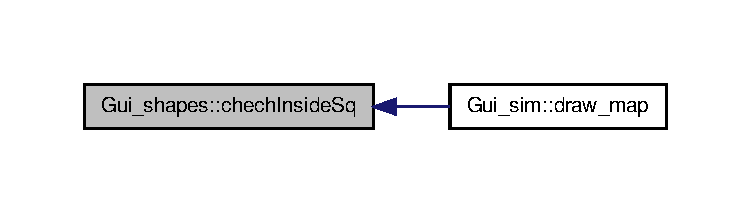
\includegraphics[width=350pt]{class_gui__shapes_a8b54490d09fe63584e74a2711d310536_icgraph}
\end{center}
\end{figure}


\hypertarget{class_gui__shapes_a5966b231784bda1913d6427591702967}{\index{Gui\-\_\-shapes@{Gui\-\_\-shapes}!draw\-\_\-circle@{draw\-\_\-circle}}
\index{draw\-\_\-circle@{draw\-\_\-circle}!Gui_shapes@{Gui\-\_\-shapes}}
\subsubsection[{draw\-\_\-circle}]{\setlength{\rightskip}{0pt plus 5cm}void Gui\-\_\-shapes\-::draw\-\_\-circle (
\begin{DoxyParamCaption}
\item[{{\bf vec3f}}]{pos, }
\item[{float}]{r, }
\item[{int}]{num\-\_\-segments}
\end{DoxyParamCaption}
)}}\label{class_gui__shapes_a5966b231784bda1913d6427591702967}
\hypertarget{class_gui__shapes_a30338d7a252b614e735e0367ea709a42}{\index{Gui\-\_\-shapes@{Gui\-\_\-shapes}!rect@{rect}}
\index{rect@{rect}!Gui_shapes@{Gui\-\_\-shapes}}
\subsubsection[{rect}]{\setlength{\rightskip}{0pt plus 5cm}void Gui\-\_\-shapes\-::rect (
\begin{DoxyParamCaption}
\item[{{\bf vec3f}}]{pos, }
\item[{float}]{hoffset, }
\item[{float}]{voffset}
\end{DoxyParamCaption}
)}}\label{class_gui__shapes_a30338d7a252b614e735e0367ea709a42}


Here is the caller graph for this function\-:\nopagebreak
\begin{figure}[H]
\begin{center}
\leavevmode
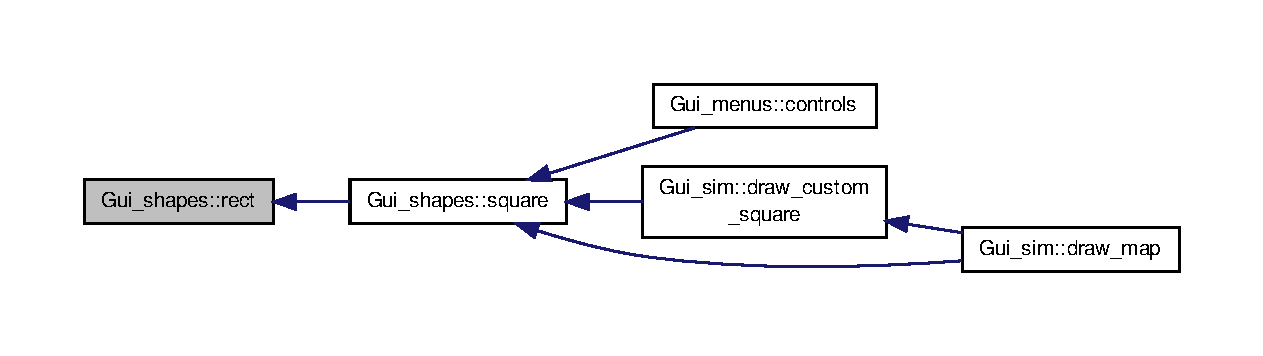
\includegraphics[width=350pt]{class_gui__shapes_a30338d7a252b614e735e0367ea709a42_icgraph}
\end{center}
\end{figure}


\hypertarget{class_gui__shapes_a64cf65d080676f4c15edf3dd169ae926}{\index{Gui\-\_\-shapes@{Gui\-\_\-shapes}!sphere@{sphere}}
\index{sphere@{sphere}!Gui_shapes@{Gui\-\_\-shapes}}
\subsubsection[{sphere}]{\setlength{\rightskip}{0pt plus 5cm}void Gui\-\_\-shapes\-::sphere (
\begin{DoxyParamCaption}
\item[{float}]{radius, }
\item[{int}]{slices, }
\item[{int}]{stacks, }
\item[{float}]{hoffset, }
\item[{float}]{voffset, }
\item[{float}]{z}
\end{DoxyParamCaption}
)}}\label{class_gui__shapes_a64cf65d080676f4c15edf3dd169ae926}
\hypertarget{class_gui__shapes_a2f9f6ec185170f2c88051bf3386af45d}{\index{Gui\-\_\-shapes@{Gui\-\_\-shapes}!square@{square}}
\index{square@{square}!Gui_shapes@{Gui\-\_\-shapes}}
\subsubsection[{square}]{\setlength{\rightskip}{0pt plus 5cm}void Gui\-\_\-shapes\-::square (
\begin{DoxyParamCaption}
\item[{float}]{side, }
\item[{float}]{z, }
\item[{float}]{hoffset, }
\item[{float}]{voffset}
\end{DoxyParamCaption}
)}}\label{class_gui__shapes_a2f9f6ec185170f2c88051bf3386af45d}


Here is the call graph for this function\-:\nopagebreak
\begin{figure}[H]
\begin{center}
\leavevmode
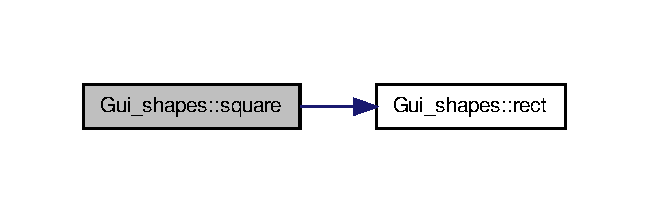
\includegraphics[width=312pt]{class_gui__shapes_a2f9f6ec185170f2c88051bf3386af45d_cgraph}
\end{center}
\end{figure}




Here is the caller graph for this function\-:\nopagebreak
\begin{figure}[H]
\begin{center}
\leavevmode
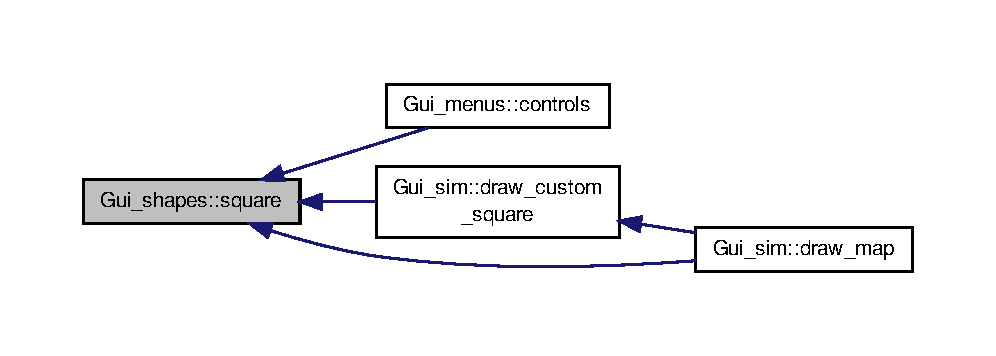
\includegraphics[width=350pt]{class_gui__shapes_a2f9f6ec185170f2c88051bf3386af45d_icgraph}
\end{center}
\end{figure}




The documentation for this class was generated from the following files\-:\begin{DoxyCompactItemize}
\item 
/home/baios/\-Cpp\-\_\-\-Projects/\-Cpp\-Ceid/include/frontend/\-Gui/\hyperlink{_gui__shapes_8h}{Gui\-\_\-shapes.\-h}\item 
/home/baios/\-Cpp\-\_\-\-Projects/\-Cpp\-Ceid/src/frontend/\-Gui/\hyperlink{_gui__shapes_8cpp}{Gui\-\_\-shapes.\-cpp}\end{DoxyCompactItemize}

\hypertarget{class_gui__sim}{\section{Gui\-\_\-sim Class Reference}
\label{class_gui__sim}\index{Gui\-\_\-sim@{Gui\-\_\-sim}}
}


{\ttfamily \#include $<$Gui\-\_\-sim.\-h$>$}



Collaboration diagram for Gui\-\_\-sim\-:
\nopagebreak
\begin{figure}[H]
\begin{center}
\leavevmode
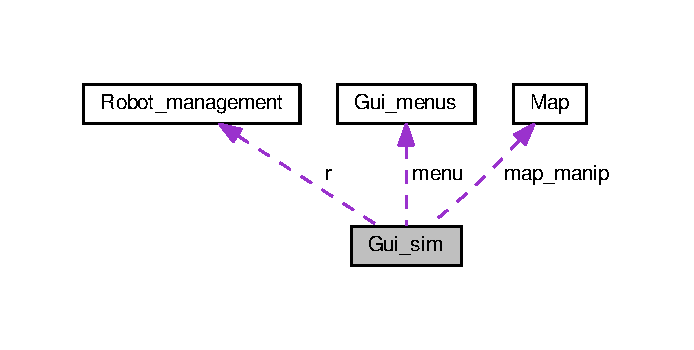
\includegraphics[width=333pt]{class_gui__sim__coll__graph}
\end{center}
\end{figure}
\subsection*{Public Member Functions}
\begin{DoxyCompactItemize}
\item 
\hyperlink{class_gui__sim_add3078535e1413f60aecc41bfc6c0074}{Gui\-\_\-sim} ()
\item 
void \hyperlink{class_gui__sim_a6ff2df84a5a1fe1daa252120c8ee4289}{init} (\hyperlink{class_map}{Map} \&m)
\item 
void \hyperlink{class_gui__sim_abb1df0449546eb8b1004a6160291ecad}{start\-\_\-new\-\_\-sim} ()
\item 
void \hyperlink{class_gui__sim_ae290c48db83ff530e74f79692a1cfc69}{run\-Sim} (bool paused, int \&vel, \hyperlink{_robot__management_8h_a4d3943ddea65db7163a58e6c7e8df95a}{uint} \&iter)
\item 
void \hyperlink{class_gui__sim_acf8e3da57fa2a597e6fed331ed7c0998}{end\-\_\-sim} ()
\item 
void \hyperlink{class_gui__sim_ac6cf2c2801ef0ed361d0c008af1af029}{draw\-\_\-map} ()
\item 
void \hyperlink{class_gui__sim_adb9a92ce767129d60069f78a5ca5aff9}{draw\-\_\-map\-\_\-dangers} (float x, float y)
\item 
void \hyperlink{class_gui__sim_a9577f2cf114ebc2575c155a83f26c826}{draw\-\_\-custom\-\_\-square} (float side, float z, float hoff, float voff, \hyperlink{_gui_8h_a199ee0f48afbd5920bf30972f7a381dc}{vec3f} colour, G\-Luint tex)
\item 
void \hyperlink{class_gui__sim_aa4d039fb6cf1bb7e6a0b42b85893836a}{set\-\_\-textures} (G\-Luint tex\mbox{[}$\,$\mbox{]})
\item 
void \hyperlink{class_gui__sim_a5e7ac19ede590bb2ac4cf2240899cdd2}{set\-\_\-alpha} (float a)
\item 
void \hyperlink{class_gui__sim_aea6641ee3522e87c4ec79467de025a0b}{set\-\_\-tile\-\_\-pressed} (float world\-\_\-x, float world\-\_\-y, float world\-\_\-z)
\item 
float \hyperlink{class_gui__sim_a3bdae000c4d601303964fb410bfbbe58}{get\-\_\-alpha} ()
\item 
void \hyperlink{class_gui__sim_a85c41961dfd75313224b4c406c308579}{get\-\_\-selected\-\_\-coord} (int \&sx, int \&sy)
\item 
void \hyperlink{class_gui__sim_ad4feb119972837ac03d9e1dbe573211e}{add\-Robot\-Pos} (char type, int x, int y)
\item 
void \hyperlink{class_gui__sim_a73467161ff658d0bd334c7245f55bebe}{remove\-Robot\-Pos} (int x, int y)
\item 
void \hyperlink{class_gui__sim_affe2de35c0ebf9b76f7c07ddd76df1c2}{move\-Robot} (int cur\-X, int cur\-Y, int target\-X, int target\-Y)
\end{DoxyCompactItemize}
\subsection*{Public Attributes}
\begin{DoxyCompactItemize}
\item 
\hyperlink{class_map}{Map} \hyperlink{class_gui__sim_ae7cb7c801fd02dbc2602252f9de2a748}{map\-\_\-manip}
\item 
\hyperlink{class_robot__management}{Robot\-\_\-management} \hyperlink{class_gui__sim_ae78a76d8502b6a79cf582769af82dbd4}{r}
\item 
\hyperlink{class_gui__menus}{Gui\-\_\-menus} \hyperlink{class_gui__sim_a45c06161fcea360f6a0beb071827e3b1}{menu}
\item 
bool \hyperlink{class_gui__sim_a2be104727246fbe590044d9dc021eb47}{selected}
\item 
bool \hyperlink{class_gui__sim_a30d3113e5b0c640c6a06c57948fbec55}{succeded}
\item 
bool \hyperlink{class_gui__sim_a2c1abe69c173fe35195a492380b77f1b}{failed}
\end{DoxyCompactItemize}


\subsection{Constructor \& Destructor Documentation}
\hypertarget{class_gui__sim_add3078535e1413f60aecc41bfc6c0074}{\index{Gui\-\_\-sim@{Gui\-\_\-sim}!Gui\-\_\-sim@{Gui\-\_\-sim}}
\index{Gui\-\_\-sim@{Gui\-\_\-sim}!Gui_sim@{Gui\-\_\-sim}}
\subsubsection[{Gui\-\_\-sim}]{\setlength{\rightskip}{0pt plus 5cm}Gui\-\_\-sim\-::\-Gui\-\_\-sim (
\begin{DoxyParamCaption}
{}
\end{DoxyParamCaption}
)}}\label{class_gui__sim_add3078535e1413f60aecc41bfc6c0074}


\subsection{Member Function Documentation}
\hypertarget{class_gui__sim_ad4feb119972837ac03d9e1dbe573211e}{\index{Gui\-\_\-sim@{Gui\-\_\-sim}!add\-Robot\-Pos@{add\-Robot\-Pos}}
\index{add\-Robot\-Pos@{add\-Robot\-Pos}!Gui_sim@{Gui\-\_\-sim}}
\subsubsection[{add\-Robot\-Pos}]{\setlength{\rightskip}{0pt plus 5cm}void Gui\-\_\-sim\-::add\-Robot\-Pos (
\begin{DoxyParamCaption}
\item[{char}]{type, }
\item[{int}]{x, }
\item[{int}]{y}
\end{DoxyParamCaption}
)}}\label{class_gui__sim_ad4feb119972837ac03d9e1dbe573211e}


Here is the call graph for this function\-:
\nopagebreak
\begin{figure}[H]
\begin{center}
\leavevmode
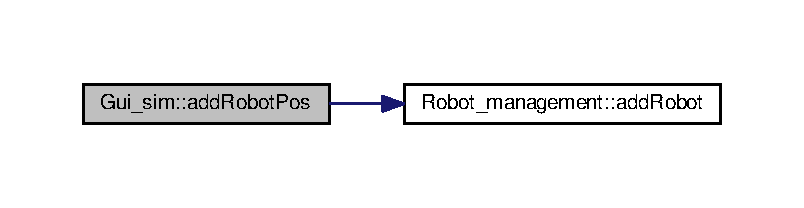
\includegraphics[width=350pt]{class_gui__sim_ad4feb119972837ac03d9e1dbe573211e_cgraph}
\end{center}
\end{figure}


\hypertarget{class_gui__sim_a9577f2cf114ebc2575c155a83f26c826}{\index{Gui\-\_\-sim@{Gui\-\_\-sim}!draw\-\_\-custom\-\_\-square@{draw\-\_\-custom\-\_\-square}}
\index{draw\-\_\-custom\-\_\-square@{draw\-\_\-custom\-\_\-square}!Gui_sim@{Gui\-\_\-sim}}
\subsubsection[{draw\-\_\-custom\-\_\-square}]{\setlength{\rightskip}{0pt plus 5cm}void Gui\-\_\-sim\-::draw\-\_\-custom\-\_\-square (
\begin{DoxyParamCaption}
\item[{float}]{side, }
\item[{float}]{z, }
\item[{float}]{hoff, }
\item[{float}]{voff, }
\item[{{\bf vec3f}}]{colour, }
\item[{G\-Luint}]{tex}
\end{DoxyParamCaption}
)}}\label{class_gui__sim_a9577f2cf114ebc2575c155a83f26c826}


Here is the call graph for this function\-:
\nopagebreak
\begin{figure}[H]
\begin{center}
\leavevmode
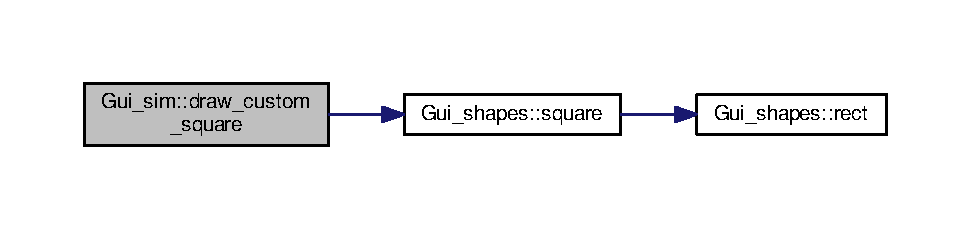
\includegraphics[width=350pt]{class_gui__sim_a9577f2cf114ebc2575c155a83f26c826_cgraph}
\end{center}
\end{figure}




Here is the caller graph for this function\-:
\nopagebreak
\begin{figure}[H]
\begin{center}
\leavevmode
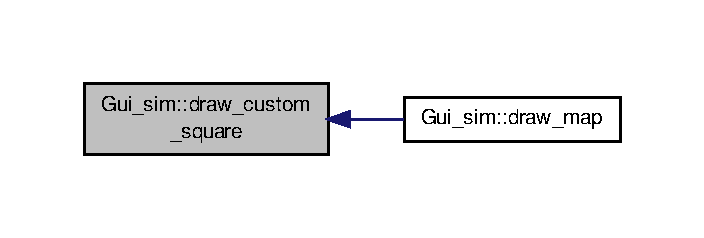
\includegraphics[width=338pt]{class_gui__sim_a9577f2cf114ebc2575c155a83f26c826_icgraph}
\end{center}
\end{figure}


\hypertarget{class_gui__sim_ac6cf2c2801ef0ed361d0c008af1af029}{\index{Gui\-\_\-sim@{Gui\-\_\-sim}!draw\-\_\-map@{draw\-\_\-map}}
\index{draw\-\_\-map@{draw\-\_\-map}!Gui_sim@{Gui\-\_\-sim}}
\subsubsection[{draw\-\_\-map}]{\setlength{\rightskip}{0pt plus 5cm}void Gui\-\_\-sim\-::draw\-\_\-map (
\begin{DoxyParamCaption}
{}
\end{DoxyParamCaption}
)}}\label{class_gui__sim_ac6cf2c2801ef0ed361d0c008af1af029}


Here is the call graph for this function\-:
\nopagebreak
\begin{figure}[H]
\begin{center}
\leavevmode
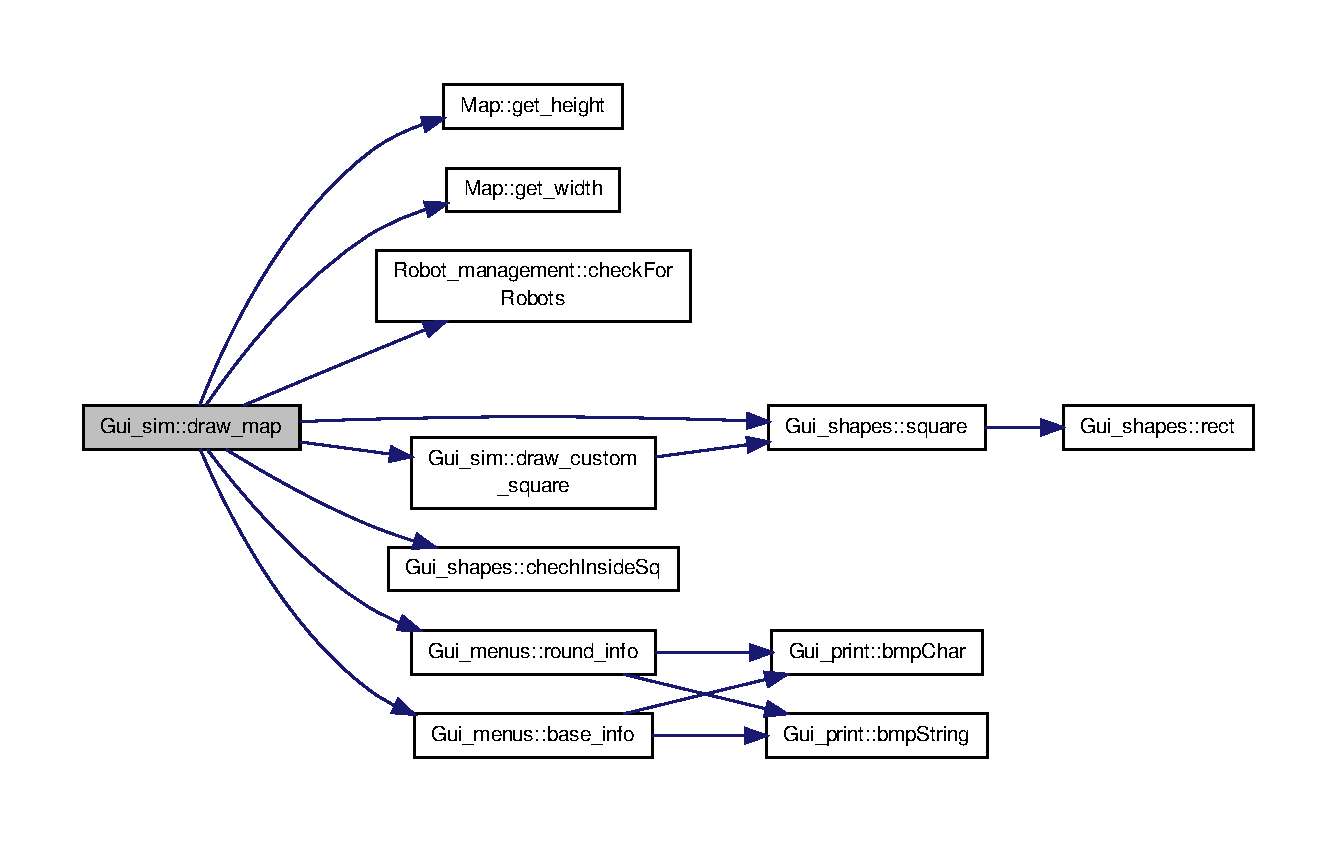
\includegraphics[width=350pt]{class_gui__sim_ac6cf2c2801ef0ed361d0c008af1af029_cgraph}
\end{center}
\end{figure}


\hypertarget{class_gui__sim_adb9a92ce767129d60069f78a5ca5aff9}{\index{Gui\-\_\-sim@{Gui\-\_\-sim}!draw\-\_\-map\-\_\-dangers@{draw\-\_\-map\-\_\-dangers}}
\index{draw\-\_\-map\-\_\-dangers@{draw\-\_\-map\-\_\-dangers}!Gui_sim@{Gui\-\_\-sim}}
\subsubsection[{draw\-\_\-map\-\_\-dangers}]{\setlength{\rightskip}{0pt plus 5cm}void Gui\-\_\-sim\-::draw\-\_\-map\-\_\-dangers (
\begin{DoxyParamCaption}
\item[{float}]{x, }
\item[{float}]{y}
\end{DoxyParamCaption}
)}}\label{class_gui__sim_adb9a92ce767129d60069f78a5ca5aff9}
\hypertarget{class_gui__sim_acf8e3da57fa2a597e6fed331ed7c0998}{\index{Gui\-\_\-sim@{Gui\-\_\-sim}!end\-\_\-sim@{end\-\_\-sim}}
\index{end\-\_\-sim@{end\-\_\-sim}!Gui_sim@{Gui\-\_\-sim}}
\subsubsection[{end\-\_\-sim}]{\setlength{\rightskip}{0pt plus 5cm}void Gui\-\_\-sim\-::end\-\_\-sim (
\begin{DoxyParamCaption}
{}
\end{DoxyParamCaption}
)}}\label{class_gui__sim_acf8e3da57fa2a597e6fed331ed7c0998}


Here is the call graph for this function\-:
\nopagebreak
\begin{figure}[H]
\begin{center}
\leavevmode
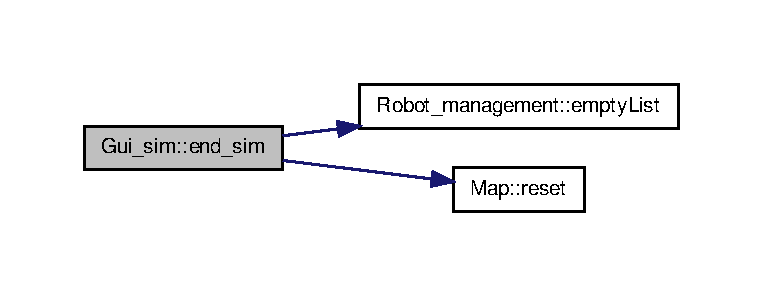
\includegraphics[width=350pt]{class_gui__sim_acf8e3da57fa2a597e6fed331ed7c0998_cgraph}
\end{center}
\end{figure}


\hypertarget{class_gui__sim_a3bdae000c4d601303964fb410bfbbe58}{\index{Gui\-\_\-sim@{Gui\-\_\-sim}!get\-\_\-alpha@{get\-\_\-alpha}}
\index{get\-\_\-alpha@{get\-\_\-alpha}!Gui_sim@{Gui\-\_\-sim}}
\subsubsection[{get\-\_\-alpha}]{\setlength{\rightskip}{0pt plus 5cm}float Gui\-\_\-sim\-::get\-\_\-alpha (
\begin{DoxyParamCaption}
{}
\end{DoxyParamCaption}
)}}\label{class_gui__sim_a3bdae000c4d601303964fb410bfbbe58}
\hypertarget{class_gui__sim_a85c41961dfd75313224b4c406c308579}{\index{Gui\-\_\-sim@{Gui\-\_\-sim}!get\-\_\-selected\-\_\-coord@{get\-\_\-selected\-\_\-coord}}
\index{get\-\_\-selected\-\_\-coord@{get\-\_\-selected\-\_\-coord}!Gui_sim@{Gui\-\_\-sim}}
\subsubsection[{get\-\_\-selected\-\_\-coord}]{\setlength{\rightskip}{0pt plus 5cm}void Gui\-\_\-sim\-::get\-\_\-selected\-\_\-coord (
\begin{DoxyParamCaption}
\item[{int \&}]{sx, }
\item[{int \&}]{sy}
\end{DoxyParamCaption}
)}}\label{class_gui__sim_a85c41961dfd75313224b4c406c308579}
\hypertarget{class_gui__sim_a6ff2df84a5a1fe1daa252120c8ee4289}{\index{Gui\-\_\-sim@{Gui\-\_\-sim}!init@{init}}
\index{init@{init}!Gui_sim@{Gui\-\_\-sim}}
\subsubsection[{init}]{\setlength{\rightskip}{0pt plus 5cm}void Gui\-\_\-sim\-::init (
\begin{DoxyParamCaption}
\item[{{\bf Map} \&}]{m}
\end{DoxyParamCaption}
)}}\label{class_gui__sim_a6ff2df84a5a1fe1daa252120c8ee4289}


Here is the call graph for this function\-:
\nopagebreak
\begin{figure}[H]
\begin{center}
\leavevmode
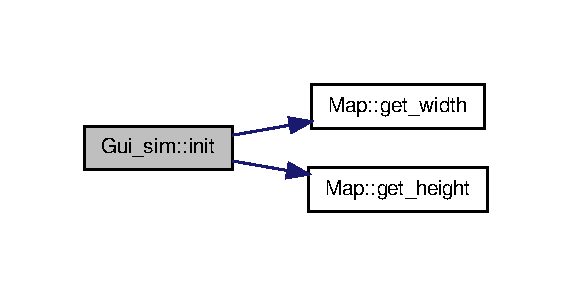
\includegraphics[width=274pt]{class_gui__sim_a6ff2df84a5a1fe1daa252120c8ee4289_cgraph}
\end{center}
\end{figure}




Here is the caller graph for this function\-:
\nopagebreak
\begin{figure}[H]
\begin{center}
\leavevmode
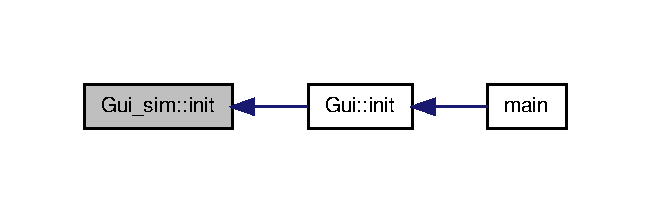
\includegraphics[width=312pt]{class_gui__sim_a6ff2df84a5a1fe1daa252120c8ee4289_icgraph}
\end{center}
\end{figure}


\hypertarget{class_gui__sim_affe2de35c0ebf9b76f7c07ddd76df1c2}{\index{Gui\-\_\-sim@{Gui\-\_\-sim}!move\-Robot@{move\-Robot}}
\index{move\-Robot@{move\-Robot}!Gui_sim@{Gui\-\_\-sim}}
\subsubsection[{move\-Robot}]{\setlength{\rightskip}{0pt plus 5cm}void Gui\-\_\-sim\-::move\-Robot (
\begin{DoxyParamCaption}
\item[{int}]{cur\-X, }
\item[{int}]{cur\-Y, }
\item[{int}]{target\-X, }
\item[{int}]{target\-Y}
\end{DoxyParamCaption}
)}}\label{class_gui__sim_affe2de35c0ebf9b76f7c07ddd76df1c2}


Here is the call graph for this function\-:
\nopagebreak
\begin{figure}[H]
\begin{center}
\leavevmode
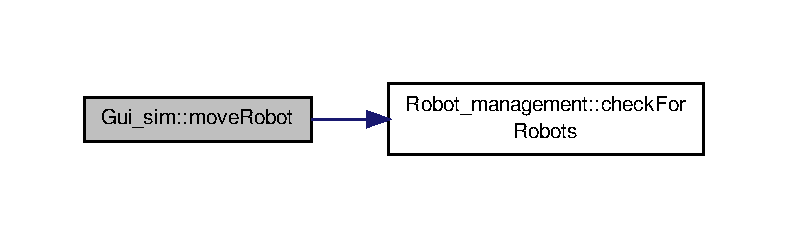
\includegraphics[width=350pt]{class_gui__sim_affe2de35c0ebf9b76f7c07ddd76df1c2_cgraph}
\end{center}
\end{figure}


\hypertarget{class_gui__sim_a73467161ff658d0bd334c7245f55bebe}{\index{Gui\-\_\-sim@{Gui\-\_\-sim}!remove\-Robot\-Pos@{remove\-Robot\-Pos}}
\index{remove\-Robot\-Pos@{remove\-Robot\-Pos}!Gui_sim@{Gui\-\_\-sim}}
\subsubsection[{remove\-Robot\-Pos}]{\setlength{\rightskip}{0pt plus 5cm}void Gui\-\_\-sim\-::remove\-Robot\-Pos (
\begin{DoxyParamCaption}
\item[{int}]{x, }
\item[{int}]{y}
\end{DoxyParamCaption}
)}}\label{class_gui__sim_a73467161ff658d0bd334c7245f55bebe}


Here is the call graph for this function\-:
\nopagebreak
\begin{figure}[H]
\begin{center}
\leavevmode
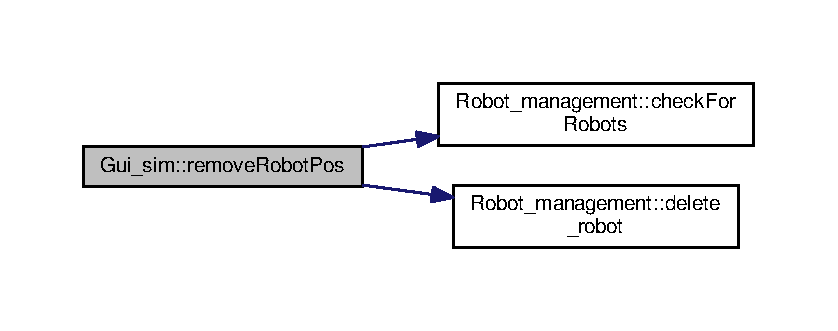
\includegraphics[width=350pt]{class_gui__sim_a73467161ff658d0bd334c7245f55bebe_cgraph}
\end{center}
\end{figure}


\hypertarget{class_gui__sim_ae290c48db83ff530e74f79692a1cfc69}{\index{Gui\-\_\-sim@{Gui\-\_\-sim}!run\-Sim@{run\-Sim}}
\index{run\-Sim@{run\-Sim}!Gui_sim@{Gui\-\_\-sim}}
\subsubsection[{run\-Sim}]{\setlength{\rightskip}{0pt plus 5cm}void Gui\-\_\-sim\-::run\-Sim (
\begin{DoxyParamCaption}
\item[{bool}]{paused, }
\item[{int \&}]{vel, }
\item[{{\bf uint} \&}]{iter}
\end{DoxyParamCaption}
)}}\label{class_gui__sim_ae290c48db83ff530e74f79692a1cfc69}


Here is the call graph for this function\-:
\nopagebreak
\begin{figure}[H]
\begin{center}
\leavevmode
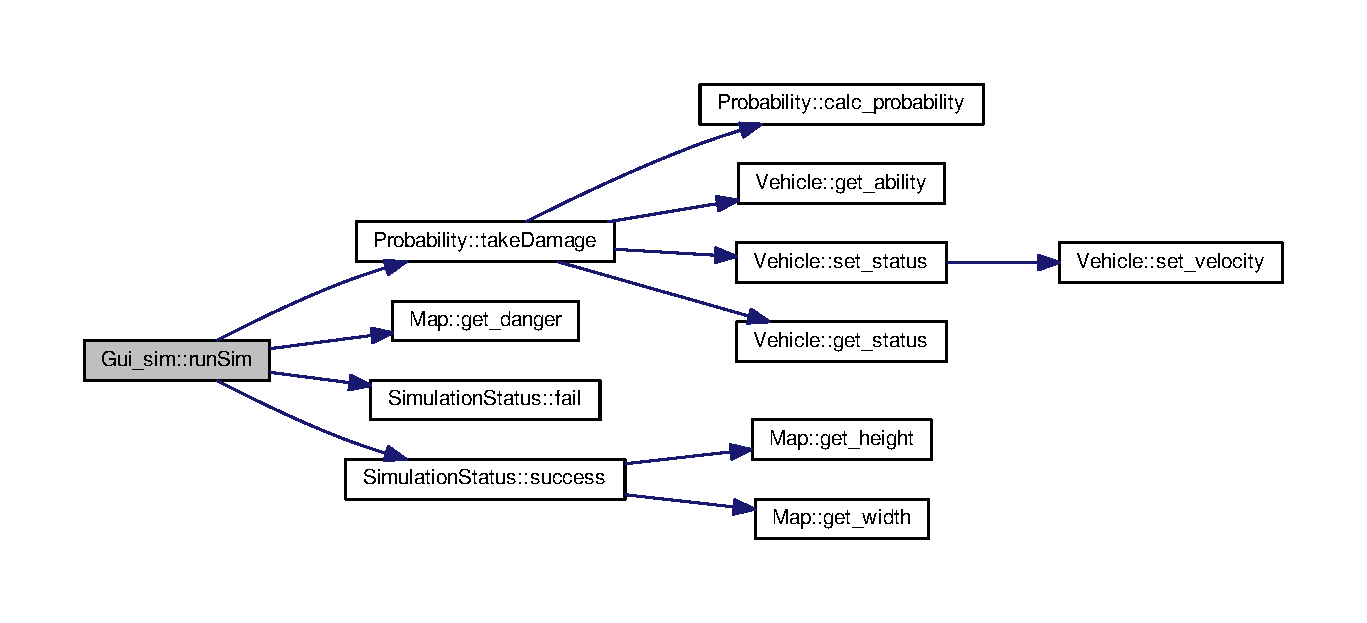
\includegraphics[width=350pt]{class_gui__sim_ae290c48db83ff530e74f79692a1cfc69_cgraph}
\end{center}
\end{figure}


\hypertarget{class_gui__sim_a5e7ac19ede590bb2ac4cf2240899cdd2}{\index{Gui\-\_\-sim@{Gui\-\_\-sim}!set\-\_\-alpha@{set\-\_\-alpha}}
\index{set\-\_\-alpha@{set\-\_\-alpha}!Gui_sim@{Gui\-\_\-sim}}
\subsubsection[{set\-\_\-alpha}]{\setlength{\rightskip}{0pt plus 5cm}void Gui\-\_\-sim\-::set\-\_\-alpha (
\begin{DoxyParamCaption}
\item[{float}]{a}
\end{DoxyParamCaption}
)}}\label{class_gui__sim_a5e7ac19ede590bb2ac4cf2240899cdd2}
\hypertarget{class_gui__sim_aa4d039fb6cf1bb7e6a0b42b85893836a}{\index{Gui\-\_\-sim@{Gui\-\_\-sim}!set\-\_\-textures@{set\-\_\-textures}}
\index{set\-\_\-textures@{set\-\_\-textures}!Gui_sim@{Gui\-\_\-sim}}
\subsubsection[{set\-\_\-textures}]{\setlength{\rightskip}{0pt plus 5cm}void Gui\-\_\-sim\-::set\-\_\-textures (
\begin{DoxyParamCaption}
\item[{G\-Luint}]{tex\mbox{[}$\,$\mbox{]}}
\end{DoxyParamCaption}
)}}\label{class_gui__sim_aa4d039fb6cf1bb7e6a0b42b85893836a}
\hypertarget{class_gui__sim_aea6641ee3522e87c4ec79467de025a0b}{\index{Gui\-\_\-sim@{Gui\-\_\-sim}!set\-\_\-tile\-\_\-pressed@{set\-\_\-tile\-\_\-pressed}}
\index{set\-\_\-tile\-\_\-pressed@{set\-\_\-tile\-\_\-pressed}!Gui_sim@{Gui\-\_\-sim}}
\subsubsection[{set\-\_\-tile\-\_\-pressed}]{\setlength{\rightskip}{0pt plus 5cm}void Gui\-\_\-sim\-::set\-\_\-tile\-\_\-pressed (
\begin{DoxyParamCaption}
\item[{float}]{world\-\_\-x, }
\item[{float}]{world\-\_\-y, }
\item[{float}]{world\-\_\-z}
\end{DoxyParamCaption}
)}}\label{class_gui__sim_aea6641ee3522e87c4ec79467de025a0b}
\hypertarget{class_gui__sim_abb1df0449546eb8b1004a6160291ecad}{\index{Gui\-\_\-sim@{Gui\-\_\-sim}!start\-\_\-new\-\_\-sim@{start\-\_\-new\-\_\-sim}}
\index{start\-\_\-new\-\_\-sim@{start\-\_\-new\-\_\-sim}!Gui_sim@{Gui\-\_\-sim}}
\subsubsection[{start\-\_\-new\-\_\-sim}]{\setlength{\rightskip}{0pt plus 5cm}void Gui\-\_\-sim\-::start\-\_\-new\-\_\-sim (
\begin{DoxyParamCaption}
{}
\end{DoxyParamCaption}
)}}\label{class_gui__sim_abb1df0449546eb8b1004a6160291ecad}


Here is the call graph for this function\-:
\nopagebreak
\begin{figure}[H]
\begin{center}
\leavevmode
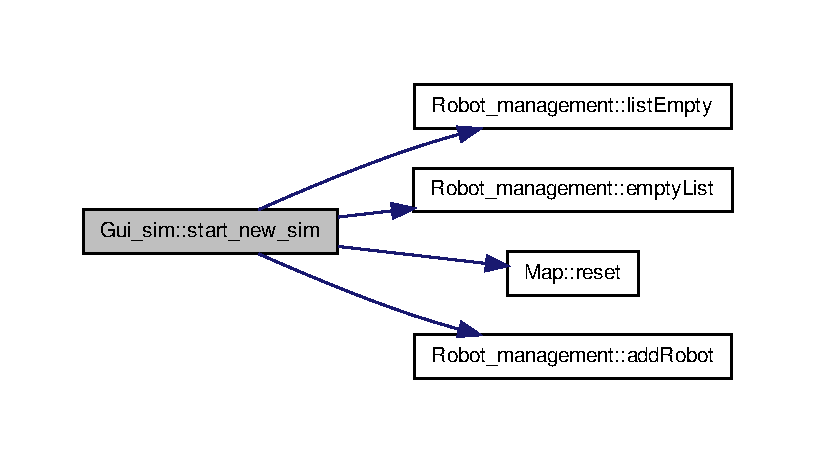
\includegraphics[width=350pt]{class_gui__sim_abb1df0449546eb8b1004a6160291ecad_cgraph}
\end{center}
\end{figure}




Here is the caller graph for this function\-:
\nopagebreak
\begin{figure}[H]
\begin{center}
\leavevmode
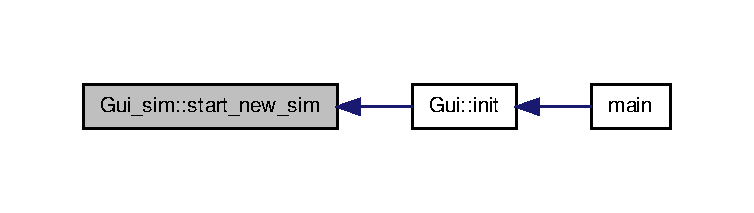
\includegraphics[width=350pt]{class_gui__sim_abb1df0449546eb8b1004a6160291ecad_icgraph}
\end{center}
\end{figure}




\subsection{Member Data Documentation}
\hypertarget{class_gui__sim_a2c1abe69c173fe35195a492380b77f1b}{\index{Gui\-\_\-sim@{Gui\-\_\-sim}!failed@{failed}}
\index{failed@{failed}!Gui_sim@{Gui\-\_\-sim}}
\subsubsection[{failed}]{\setlength{\rightskip}{0pt plus 5cm}bool Gui\-\_\-sim\-::failed}}\label{class_gui__sim_a2c1abe69c173fe35195a492380b77f1b}
\hypertarget{class_gui__sim_ae7cb7c801fd02dbc2602252f9de2a748}{\index{Gui\-\_\-sim@{Gui\-\_\-sim}!map\-\_\-manip@{map\-\_\-manip}}
\index{map\-\_\-manip@{map\-\_\-manip}!Gui_sim@{Gui\-\_\-sim}}
\subsubsection[{map\-\_\-manip}]{\setlength{\rightskip}{0pt plus 5cm}{\bf Map} Gui\-\_\-sim\-::map\-\_\-manip}}\label{class_gui__sim_ae7cb7c801fd02dbc2602252f9de2a748}
\hypertarget{class_gui__sim_a45c06161fcea360f6a0beb071827e3b1}{\index{Gui\-\_\-sim@{Gui\-\_\-sim}!menu@{menu}}
\index{menu@{menu}!Gui_sim@{Gui\-\_\-sim}}
\subsubsection[{menu}]{\setlength{\rightskip}{0pt plus 5cm}{\bf Gui\-\_\-menus} Gui\-\_\-sim\-::menu}}\label{class_gui__sim_a45c06161fcea360f6a0beb071827e3b1}
\hypertarget{class_gui__sim_ae78a76d8502b6a79cf582769af82dbd4}{\index{Gui\-\_\-sim@{Gui\-\_\-sim}!r@{r}}
\index{r@{r}!Gui_sim@{Gui\-\_\-sim}}
\subsubsection[{r}]{\setlength{\rightskip}{0pt plus 5cm}{\bf Robot\-\_\-management} Gui\-\_\-sim\-::r}}\label{class_gui__sim_ae78a76d8502b6a79cf582769af82dbd4}
\hypertarget{class_gui__sim_a2be104727246fbe590044d9dc021eb47}{\index{Gui\-\_\-sim@{Gui\-\_\-sim}!selected@{selected}}
\index{selected@{selected}!Gui_sim@{Gui\-\_\-sim}}
\subsubsection[{selected}]{\setlength{\rightskip}{0pt plus 5cm}bool Gui\-\_\-sim\-::selected}}\label{class_gui__sim_a2be104727246fbe590044d9dc021eb47}
\hypertarget{class_gui__sim_a30d3113e5b0c640c6a06c57948fbec55}{\index{Gui\-\_\-sim@{Gui\-\_\-sim}!succeded@{succeded}}
\index{succeded@{succeded}!Gui_sim@{Gui\-\_\-sim}}
\subsubsection[{succeded}]{\setlength{\rightskip}{0pt plus 5cm}bool Gui\-\_\-sim\-::succeded}}\label{class_gui__sim_a30d3113e5b0c640c6a06c57948fbec55}


The documentation for this class was generated from the following files\-:\begin{DoxyCompactItemize}
\item 
/home/baios/\-Desktop/robsim/\-Rob\-Sim/include/frontend/\-Gui/\hyperlink{_gui__sim_8h}{Gui\-\_\-sim.\-h}\item 
/home/baios/\-Desktop/robsim/\-Rob\-Sim/src/frontend/\-Gui/\hyperlink{_gui__sim_8cpp}{Gui\-\_\-sim.\-cpp}\end{DoxyCompactItemize}

\hypertarget{class_gui__textures}{\section{Gui\-\_\-textures Class Reference}
\label{class_gui__textures}\index{Gui\-\_\-textures@{Gui\-\_\-textures}}
}


{\ttfamily \#include $<$Gui\-\_\-textures.\-h$>$}

\subsection*{Public Member Functions}
\begin{DoxyCompactItemize}
\item 
\hyperlink{class_gui__textures_adbc7e0cc3f7aa8498d25e8944afa7386}{Gui\-\_\-textures} ()
\item 
G\-Luint \hyperlink{class_gui__textures_aec95484eb468423df6f179fde5877886}{load\-Epic\-Tex} (std\-::string filename)
\item 
void \hyperlink{class_gui__textures_a1e228d12b9d28fa92c4749ed286321d8}{draw\-Epic\-Background} ()
\end{DoxyCompactItemize}


\subsection{Constructor \& Destructor Documentation}
\hypertarget{class_gui__textures_adbc7e0cc3f7aa8498d25e8944afa7386}{\index{Gui\-\_\-textures@{Gui\-\_\-textures}!Gui\-\_\-textures@{Gui\-\_\-textures}}
\index{Gui\-\_\-textures@{Gui\-\_\-textures}!Gui_textures@{Gui\-\_\-textures}}
\subsubsection[{Gui\-\_\-textures}]{\setlength{\rightskip}{0pt plus 5cm}Gui\-\_\-textures\-::\-Gui\-\_\-textures (
\begin{DoxyParamCaption}
{}
\end{DoxyParamCaption}
)}}\label{class_gui__textures_adbc7e0cc3f7aa8498d25e8944afa7386}


\subsection{Member Function Documentation}
\hypertarget{class_gui__textures_a1e228d12b9d28fa92c4749ed286321d8}{\index{Gui\-\_\-textures@{Gui\-\_\-textures}!draw\-Epic\-Background@{draw\-Epic\-Background}}
\index{draw\-Epic\-Background@{draw\-Epic\-Background}!Gui_textures@{Gui\-\_\-textures}}
\subsubsection[{draw\-Epic\-Background}]{\setlength{\rightskip}{0pt plus 5cm}void Gui\-\_\-textures\-::draw\-Epic\-Background (
\begin{DoxyParamCaption}
{}
\end{DoxyParamCaption}
)}}\label{class_gui__textures_a1e228d12b9d28fa92c4749ed286321d8}
\hypertarget{class_gui__textures_aec95484eb468423df6f179fde5877886}{\index{Gui\-\_\-textures@{Gui\-\_\-textures}!load\-Epic\-Tex@{load\-Epic\-Tex}}
\index{load\-Epic\-Tex@{load\-Epic\-Tex}!Gui_textures@{Gui\-\_\-textures}}
\subsubsection[{load\-Epic\-Tex}]{\setlength{\rightskip}{0pt plus 5cm}G\-Luint Gui\-\_\-textures\-::load\-Epic\-Tex (
\begin{DoxyParamCaption}
\item[{std\-::string}]{filename}
\end{DoxyParamCaption}
)}}\label{class_gui__textures_aec95484eb468423df6f179fde5877886}


The documentation for this class was generated from the following files\-:\begin{DoxyCompactItemize}
\item 
/home/baios/\-Desktop/robsim/\-Rob\-Sim/include/frontend/\-Gui/\hyperlink{_gui__textures_8h}{Gui\-\_\-textures.\-h}\item 
/home/baios/\-Desktop/robsim/\-Rob\-Sim/src/frontend/\-Gui/\hyperlink{_gui__textures_8cpp}{Gui\-\_\-textures.\-cpp}\end{DoxyCompactItemize}

\hypertarget{class_gui__vector3f}{\section{Gui\-\_\-vector3f Class Reference}
\label{class_gui__vector3f}\index{Gui\-\_\-vector3f@{Gui\-\_\-vector3f}}
}


{\ttfamily \#include $<$Gui\-\_\-vector3f.\-h$>$}

\subsection*{Public Member Functions}
\begin{DoxyCompactItemize}
\item 
\hyperlink{class_gui__vector3f_a36f8a218666fe4c979b35d4c3c0191dc}{Gui\-\_\-vector3f} ()
\item 
\hyperlink{class_gui__vector3f_a9fcb1b9661c69b06d2be77a162322ee5}{Gui\-\_\-vector3f} (float nx, float ny, float nz)
\item 
\hyperlink{class_gui__vector3f_a298abf0fa1f67166f706a1b6f445b9b4}{Gui\-\_\-vector3f} (float nx, float ny, float nz, float nalpha)
\end{DoxyCompactItemize}
\subsection*{Public Attributes}
\begin{DoxyCompactItemize}
\item 
float \hyperlink{class_gui__vector3f_a023856935269d19fbe9e4e2405c4a330}{x}
\item 
float \hyperlink{class_gui__vector3f_aeeb2c025e216e05450ccc0516a31339c}{y}
\item 
float \hyperlink{class_gui__vector3f_a36f4373054963a96e658d27b00ccc281}{z}
\item 
float \hyperlink{class_gui__vector3f_af93c521b147e54d6b50f6612927e5d90}{alpha}
\end{DoxyCompactItemize}


\subsection{Constructor \& Destructor Documentation}
\hypertarget{class_gui__vector3f_a36f8a218666fe4c979b35d4c3c0191dc}{\index{Gui\-\_\-vector3f@{Gui\-\_\-vector3f}!Gui\-\_\-vector3f@{Gui\-\_\-vector3f}}
\index{Gui\-\_\-vector3f@{Gui\-\_\-vector3f}!Gui_vector3f@{Gui\-\_\-vector3f}}
\subsubsection[{Gui\-\_\-vector3f}]{\setlength{\rightskip}{0pt plus 5cm}Gui\-\_\-vector3f\-::\-Gui\-\_\-vector3f (
\begin{DoxyParamCaption}
{}
\end{DoxyParamCaption}
)}}\label{class_gui__vector3f_a36f8a218666fe4c979b35d4c3c0191dc}
\hypertarget{class_gui__vector3f_a9fcb1b9661c69b06d2be77a162322ee5}{\index{Gui\-\_\-vector3f@{Gui\-\_\-vector3f}!Gui\-\_\-vector3f@{Gui\-\_\-vector3f}}
\index{Gui\-\_\-vector3f@{Gui\-\_\-vector3f}!Gui_vector3f@{Gui\-\_\-vector3f}}
\subsubsection[{Gui\-\_\-vector3f}]{\setlength{\rightskip}{0pt plus 5cm}Gui\-\_\-vector3f\-::\-Gui\-\_\-vector3f (
\begin{DoxyParamCaption}
\item[{float}]{nx, }
\item[{float}]{ny, }
\item[{float}]{nz}
\end{DoxyParamCaption}
)}}\label{class_gui__vector3f_a9fcb1b9661c69b06d2be77a162322ee5}
\hypertarget{class_gui__vector3f_a298abf0fa1f67166f706a1b6f445b9b4}{\index{Gui\-\_\-vector3f@{Gui\-\_\-vector3f}!Gui\-\_\-vector3f@{Gui\-\_\-vector3f}}
\index{Gui\-\_\-vector3f@{Gui\-\_\-vector3f}!Gui_vector3f@{Gui\-\_\-vector3f}}
\subsubsection[{Gui\-\_\-vector3f}]{\setlength{\rightskip}{0pt plus 5cm}Gui\-\_\-vector3f\-::\-Gui\-\_\-vector3f (
\begin{DoxyParamCaption}
\item[{float}]{nx, }
\item[{float}]{ny, }
\item[{float}]{nz, }
\item[{float}]{nalpha}
\end{DoxyParamCaption}
)}}\label{class_gui__vector3f_a298abf0fa1f67166f706a1b6f445b9b4}


\subsection{Member Data Documentation}
\hypertarget{class_gui__vector3f_af93c521b147e54d6b50f6612927e5d90}{\index{Gui\-\_\-vector3f@{Gui\-\_\-vector3f}!alpha@{alpha}}
\index{alpha@{alpha}!Gui_vector3f@{Gui\-\_\-vector3f}}
\subsubsection[{alpha}]{\setlength{\rightskip}{0pt plus 5cm}float Gui\-\_\-vector3f\-::alpha}}\label{class_gui__vector3f_af93c521b147e54d6b50f6612927e5d90}
\hypertarget{class_gui__vector3f_a023856935269d19fbe9e4e2405c4a330}{\index{Gui\-\_\-vector3f@{Gui\-\_\-vector3f}!x@{x}}
\index{x@{x}!Gui_vector3f@{Gui\-\_\-vector3f}}
\subsubsection[{x}]{\setlength{\rightskip}{0pt plus 5cm}float Gui\-\_\-vector3f\-::x}}\label{class_gui__vector3f_a023856935269d19fbe9e4e2405c4a330}
\hypertarget{class_gui__vector3f_aeeb2c025e216e05450ccc0516a31339c}{\index{Gui\-\_\-vector3f@{Gui\-\_\-vector3f}!y@{y}}
\index{y@{y}!Gui_vector3f@{Gui\-\_\-vector3f}}
\subsubsection[{y}]{\setlength{\rightskip}{0pt plus 5cm}float Gui\-\_\-vector3f\-::y}}\label{class_gui__vector3f_aeeb2c025e216e05450ccc0516a31339c}
\hypertarget{class_gui__vector3f_a36f4373054963a96e658d27b00ccc281}{\index{Gui\-\_\-vector3f@{Gui\-\_\-vector3f}!z@{z}}
\index{z@{z}!Gui_vector3f@{Gui\-\_\-vector3f}}
\subsubsection[{z}]{\setlength{\rightskip}{0pt plus 5cm}float Gui\-\_\-vector3f\-::z}}\label{class_gui__vector3f_a36f4373054963a96e658d27b00ccc281}


The documentation for this class was generated from the following files\-:\begin{DoxyCompactItemize}
\item 
/home/baios/\-Desktop/robsim/\-Rob\-Sim/include/frontend/\-Gui/\hyperlink{_gui__vector3f_8h}{Gui\-\_\-vector3f.\-h}\item 
/home/baios/\-Desktop/robsim/\-Rob\-Sim/src/frontend/\-Gui/\hyperlink{_gui__vector3f_8cpp}{Gui\-\_\-vector3f.\-cpp}\end{DoxyCompactItemize}

\hypertarget{class_looper}{\section{Looper Class Reference}
\label{class_looper}\index{Looper@{Looper}}
}


{\ttfamily \#include $<$Looper.\-h$>$}

\subsection*{Public Member Functions}
\begin{DoxyCompactItemize}
\item 
void \hyperlink{class_looper_a5b74345ab8e4090f421378cdd71f03bd}{changemode} (int dir)
\item 
int \hyperlink{class_looper_ac82554a463703052e42e2d80c1d14cfb}{kbhit} ()
\end{DoxyCompactItemize}


\subsection{Member Function Documentation}
\hypertarget{class_looper_a5b74345ab8e4090f421378cdd71f03bd}{\index{Looper@{Looper}!changemode@{changemode}}
\index{changemode@{changemode}!Looper@{Looper}}
\subsubsection[{changemode}]{\setlength{\rightskip}{0pt plus 5cm}void Looper\-::changemode (
\begin{DoxyParamCaption}
\item[{int}]{dir}
\end{DoxyParamCaption}
)}}\label{class_looper_a5b74345ab8e4090f421378cdd71f03bd}
\hypertarget{class_looper_ac82554a463703052e42e2d80c1d14cfb}{\index{Looper@{Looper}!kbhit@{kbhit}}
\index{kbhit@{kbhit}!Looper@{Looper}}
\subsubsection[{kbhit}]{\setlength{\rightskip}{0pt plus 5cm}int Looper\-::kbhit (
\begin{DoxyParamCaption}
{}
\end{DoxyParamCaption}
)}}\label{class_looper_ac82554a463703052e42e2d80c1d14cfb}


The documentation for this class was generated from the following files\-:\begin{DoxyCompactItemize}
\item 
/home/baios/\-Cpp\-\_\-\-Projects/\-Cpp\-Ceid/include/backend/\hyperlink{_looper_8h}{Looper.\-h}\item 
/home/baios/\-Cpp\-\_\-\-Projects/\-Cpp\-Ceid/src/backend/\hyperlink{_looper_8cpp}{Looper.\-cpp}\end{DoxyCompactItemize}

\hypertarget{class_map}{\section{Map Class Reference}
\label{class_map}\index{Map@{Map}}
}


{\ttfamily \#include $<$Map.\-h$>$}

\subsection*{Public Member Functions}
\begin{DoxyCompactItemize}
\item 
\hyperlink{class_map_a7dd574b3746a45123fd765945b6a2a7e}{Map} (int x, int y)
\item 
\hyperlink{class_map_ac6a049d836102c0afb564d17b607c67d}{Map} (const \hyperlink{class_map}{Map} \&v)
\item 
\hyperlink{class_map_aa403fbe09394ccf39747588f5168e3b2}{$\sim$\-Map} ()
\item 
\hyperlink{class_map}{Map} \& \hyperlink{class_map_ad1736115fa1c828435ff37df2bb58a0f}{operator=} (const \hyperlink{class_map}{Map} \&m)
\item 
int \hyperlink{class_map_ac33fd4c3249329f4a6d4209046df6dce}{get\-\_\-size\-\_\-x} ()
\item 
int \hyperlink{class_map_a357e44a02b0dc02c139d7207b038a4a3}{get\-\_\-size\-\_\-y} ()
\item 
float \hyperlink{class_map_a1c6b0a40d53eab7cdba41b705a1cce11}{get\-\_\-danger} (int x, int y)
\item 
float \hyperlink{class_map_ac43390d491e18d220a3d94363fdb5ebf}{get\-\_\-average\-\_\-danger} ()
\item 
int \hyperlink{class_map_a38609ea6ce07bc5bb2ea55db6580b355}{get\-\_\-width} ()
\item 
int \hyperlink{class_map_adef9516dd475e67aa7f819a6a358f668}{get\-\_\-height} ()
\item 
void \hyperlink{class_map_a745c069d781baa58e6fc07d5e99ef2ca}{edit\-\_\-resources\-\_\-xy} (int x, int y, float p, float g, float i)
\item 
void \hyperlink{class_map_adc8268424092e8099647d07dfc0a5a14}{edit\-\_\-dangers\-\_\-xy} (int x, int y, float danger\-\_\-)
\item 
void \hyperlink{class_map_a904c445fdce79257fedeba09070cf88a}{reset} ()
\end{DoxyCompactItemize}
\subsection*{Public Attributes}
\begin{DoxyCompactItemize}
\item 
bool $\ast$$\ast$ \hyperlink{class_map_a496e559b2c5898e1622c962e6aa5e070}{flags}
\item 
float $\ast$$\ast$ \hyperlink{class_map_a72f5c51d7ba90727fcdff153b480c187}{dangers}
\item 
float $\ast$$\ast$ \hyperlink{class_map_a910f29ebb50c629a05c0945eb6c785ea}{resources\-\_\-p}
\item 
float $\ast$$\ast$ \hyperlink{class_map_a49a8163af842ed1d63f5d3d842f43c89}{resources\-\_\-g}
\item 
float $\ast$$\ast$ \hyperlink{class_map_a12ce9d7050191ba2f084e7e11cc41ab5}{resources\-\_\-i}
\item 
float $\ast$ \hyperlink{class_map_a9fc5f65a162ff0459b3d23ba33b2b1e1}{base\-\_\-res}
\end{DoxyCompactItemize}


\subsection{Constructor \& Destructor Documentation}
\hypertarget{class_map_a7dd574b3746a45123fd765945b6a2a7e}{\index{Map@{Map}!Map@{Map}}
\index{Map@{Map}!Map@{Map}}
\subsubsection[{Map}]{\setlength{\rightskip}{0pt plus 5cm}Map\-::\-Map (
\begin{DoxyParamCaption}
\item[{int}]{x, }
\item[{int}]{y}
\end{DoxyParamCaption}
)}}\label{class_map_a7dd574b3746a45123fd765945b6a2a7e}
\hypertarget{class_map_ac6a049d836102c0afb564d17b607c67d}{\index{Map@{Map}!Map@{Map}}
\index{Map@{Map}!Map@{Map}}
\subsubsection[{Map}]{\setlength{\rightskip}{0pt plus 5cm}Map\-::\-Map (
\begin{DoxyParamCaption}
\item[{const {\bf Map} \&}]{v}
\end{DoxyParamCaption}
)}}\label{class_map_ac6a049d836102c0afb564d17b607c67d}
\hypertarget{class_map_aa403fbe09394ccf39747588f5168e3b2}{\index{Map@{Map}!$\sim$\-Map@{$\sim$\-Map}}
\index{$\sim$\-Map@{$\sim$\-Map}!Map@{Map}}
\subsubsection[{$\sim$\-Map}]{\setlength{\rightskip}{0pt plus 5cm}Map\-::$\sim$\-Map (
\begin{DoxyParamCaption}
{}
\end{DoxyParamCaption}
)}}\label{class_map_aa403fbe09394ccf39747588f5168e3b2}


\subsection{Member Function Documentation}
\hypertarget{class_map_adc8268424092e8099647d07dfc0a5a14}{\index{Map@{Map}!edit\-\_\-dangers\-\_\-xy@{edit\-\_\-dangers\-\_\-xy}}
\index{edit\-\_\-dangers\-\_\-xy@{edit\-\_\-dangers\-\_\-xy}!Map@{Map}}
\subsubsection[{edit\-\_\-dangers\-\_\-xy}]{\setlength{\rightskip}{0pt plus 5cm}void Map\-::edit\-\_\-dangers\-\_\-xy (
\begin{DoxyParamCaption}
\item[{int}]{x, }
\item[{int}]{y, }
\item[{float}]{danger\-\_\-}
\end{DoxyParamCaption}
)}}\label{class_map_adc8268424092e8099647d07dfc0a5a14}
\hypertarget{class_map_a745c069d781baa58e6fc07d5e99ef2ca}{\index{Map@{Map}!edit\-\_\-resources\-\_\-xy@{edit\-\_\-resources\-\_\-xy}}
\index{edit\-\_\-resources\-\_\-xy@{edit\-\_\-resources\-\_\-xy}!Map@{Map}}
\subsubsection[{edit\-\_\-resources\-\_\-xy}]{\setlength{\rightskip}{0pt plus 5cm}void Map\-::edit\-\_\-resources\-\_\-xy (
\begin{DoxyParamCaption}
\item[{int}]{x, }
\item[{int}]{y, }
\item[{float}]{p, }
\item[{float}]{g, }
\item[{float}]{i}
\end{DoxyParamCaption}
)}}\label{class_map_a745c069d781baa58e6fc07d5e99ef2ca}
\hypertarget{class_map_ac43390d491e18d220a3d94363fdb5ebf}{\index{Map@{Map}!get\-\_\-average\-\_\-danger@{get\-\_\-average\-\_\-danger}}
\index{get\-\_\-average\-\_\-danger@{get\-\_\-average\-\_\-danger}!Map@{Map}}
\subsubsection[{get\-\_\-average\-\_\-danger}]{\setlength{\rightskip}{0pt plus 5cm}float Map\-::get\-\_\-average\-\_\-danger (
\begin{DoxyParamCaption}
{}
\end{DoxyParamCaption}
)}}\label{class_map_ac43390d491e18d220a3d94363fdb5ebf}


Here is the caller graph for this function\-:
\nopagebreak
\begin{figure}[H]
\begin{center}
\leavevmode
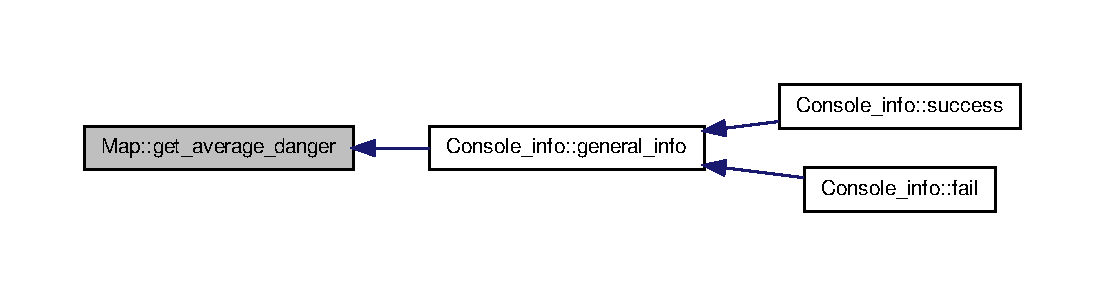
\includegraphics[width=350pt]{class_map_ac43390d491e18d220a3d94363fdb5ebf_icgraph}
\end{center}
\end{figure}


\hypertarget{class_map_a1c6b0a40d53eab7cdba41b705a1cce11}{\index{Map@{Map}!get\-\_\-danger@{get\-\_\-danger}}
\index{get\-\_\-danger@{get\-\_\-danger}!Map@{Map}}
\subsubsection[{get\-\_\-danger}]{\setlength{\rightskip}{0pt plus 5cm}float Map\-::get\-\_\-danger (
\begin{DoxyParamCaption}
\item[{int}]{x, }
\item[{int}]{y}
\end{DoxyParamCaption}
)}}\label{class_map_a1c6b0a40d53eab7cdba41b705a1cce11}


Here is the caller graph for this function\-:
\nopagebreak
\begin{figure}[H]
\begin{center}
\leavevmode
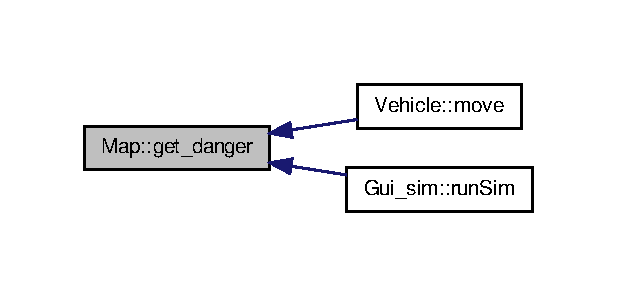
\includegraphics[width=296pt]{class_map_a1c6b0a40d53eab7cdba41b705a1cce11_icgraph}
\end{center}
\end{figure}


\hypertarget{class_map_adef9516dd475e67aa7f819a6a358f668}{\index{Map@{Map}!get\-\_\-height@{get\-\_\-height}}
\index{get\-\_\-height@{get\-\_\-height}!Map@{Map}}
\subsubsection[{get\-\_\-height}]{\setlength{\rightskip}{0pt plus 5cm}int Map\-::get\-\_\-height (
\begin{DoxyParamCaption}
{}
\end{DoxyParamCaption}
)}}\label{class_map_adef9516dd475e67aa7f819a6a358f668}


Here is the caller graph for this function\-:
\nopagebreak
\begin{figure}[H]
\begin{center}
\leavevmode
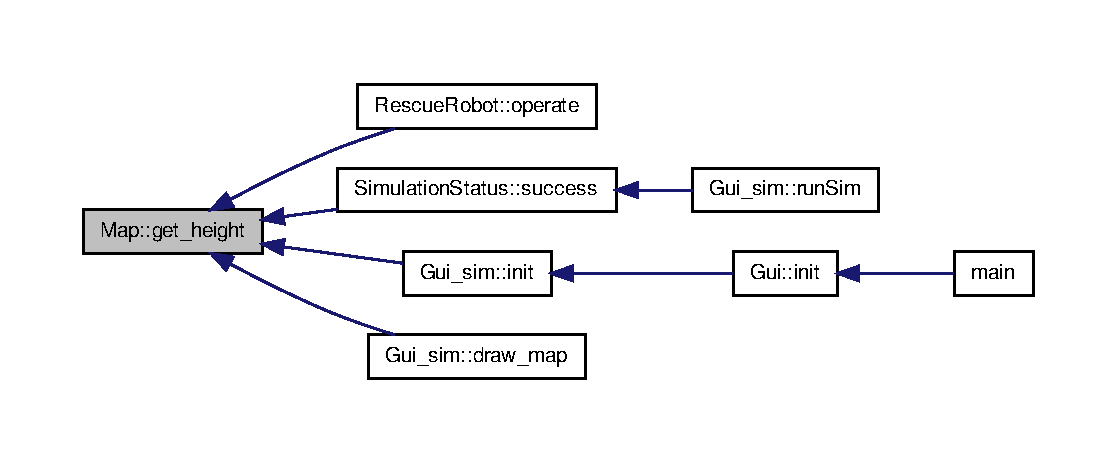
\includegraphics[width=350pt]{class_map_adef9516dd475e67aa7f819a6a358f668_icgraph}
\end{center}
\end{figure}


\hypertarget{class_map_ac33fd4c3249329f4a6d4209046df6dce}{\index{Map@{Map}!get\-\_\-size\-\_\-x@{get\-\_\-size\-\_\-x}}
\index{get\-\_\-size\-\_\-x@{get\-\_\-size\-\_\-x}!Map@{Map}}
\subsubsection[{get\-\_\-size\-\_\-x}]{\setlength{\rightskip}{0pt plus 5cm}int Map\-::get\-\_\-size\-\_\-x (
\begin{DoxyParamCaption}
{}
\end{DoxyParamCaption}
)}}\label{class_map_ac33fd4c3249329f4a6d4209046df6dce}


Here is the caller graph for this function\-:
\nopagebreak
\begin{figure}[H]
\begin{center}
\leavevmode
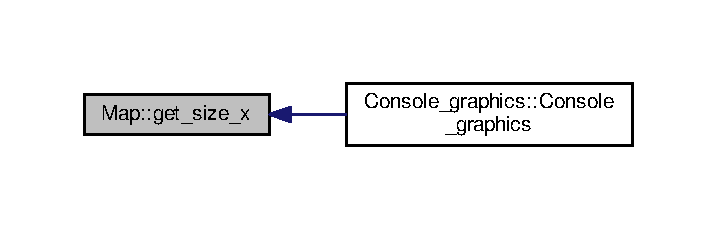
\includegraphics[width=344pt]{class_map_ac33fd4c3249329f4a6d4209046df6dce_icgraph}
\end{center}
\end{figure}


\hypertarget{class_map_a357e44a02b0dc02c139d7207b038a4a3}{\index{Map@{Map}!get\-\_\-size\-\_\-y@{get\-\_\-size\-\_\-y}}
\index{get\-\_\-size\-\_\-y@{get\-\_\-size\-\_\-y}!Map@{Map}}
\subsubsection[{get\-\_\-size\-\_\-y}]{\setlength{\rightskip}{0pt plus 5cm}int Map\-::get\-\_\-size\-\_\-y (
\begin{DoxyParamCaption}
{}
\end{DoxyParamCaption}
)}}\label{class_map_a357e44a02b0dc02c139d7207b038a4a3}


Here is the caller graph for this function\-:
\nopagebreak
\begin{figure}[H]
\begin{center}
\leavevmode
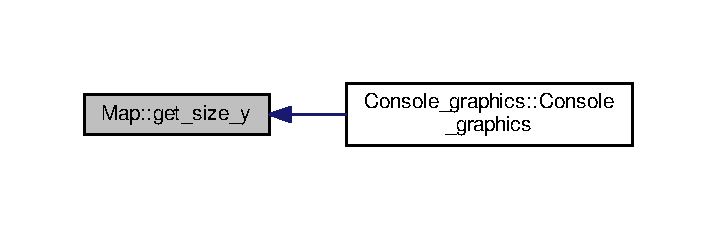
\includegraphics[width=344pt]{class_map_a357e44a02b0dc02c139d7207b038a4a3_icgraph}
\end{center}
\end{figure}


\hypertarget{class_map_a38609ea6ce07bc5bb2ea55db6580b355}{\index{Map@{Map}!get\-\_\-width@{get\-\_\-width}}
\index{get\-\_\-width@{get\-\_\-width}!Map@{Map}}
\subsubsection[{get\-\_\-width}]{\setlength{\rightskip}{0pt plus 5cm}int Map\-::get\-\_\-width (
\begin{DoxyParamCaption}
{}
\end{DoxyParamCaption}
)}}\label{class_map_a38609ea6ce07bc5bb2ea55db6580b355}


Here is the caller graph for this function\-:
\nopagebreak
\begin{figure}[H]
\begin{center}
\leavevmode
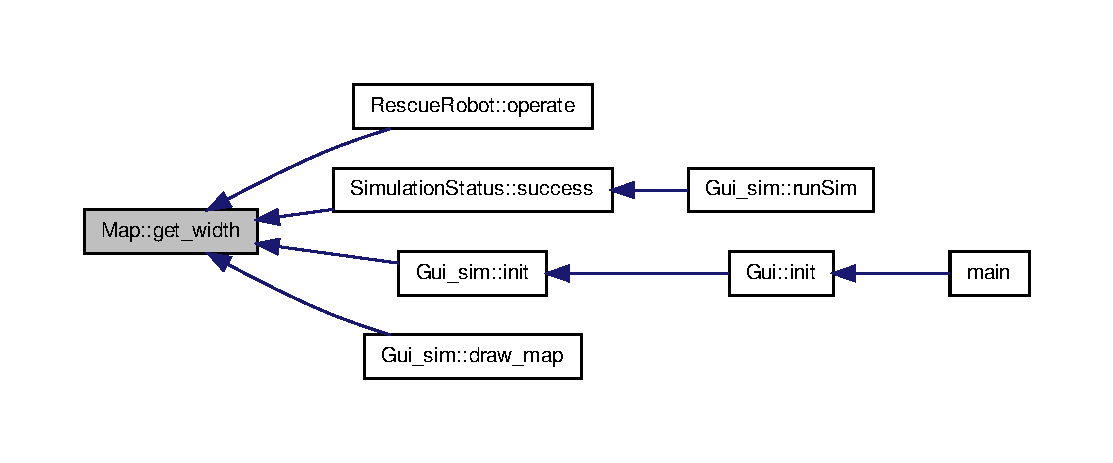
\includegraphics[width=350pt]{class_map_a38609ea6ce07bc5bb2ea55db6580b355_icgraph}
\end{center}
\end{figure}


\hypertarget{class_map_ad1736115fa1c828435ff37df2bb58a0f}{\index{Map@{Map}!operator=@{operator=}}
\index{operator=@{operator=}!Map@{Map}}
\subsubsection[{operator=}]{\setlength{\rightskip}{0pt plus 5cm}{\bf Map} \& Map\-::operator= (
\begin{DoxyParamCaption}
\item[{const {\bf Map} \&}]{m}
\end{DoxyParamCaption}
)}}\label{class_map_ad1736115fa1c828435ff37df2bb58a0f}
\hypertarget{class_map_a904c445fdce79257fedeba09070cf88a}{\index{Map@{Map}!reset@{reset}}
\index{reset@{reset}!Map@{Map}}
\subsubsection[{reset}]{\setlength{\rightskip}{0pt plus 5cm}void Map\-::reset (
\begin{DoxyParamCaption}
{}
\end{DoxyParamCaption}
)}}\label{class_map_a904c445fdce79257fedeba09070cf88a}


Here is the caller graph for this function\-:
\nopagebreak
\begin{figure}[H]
\begin{center}
\leavevmode
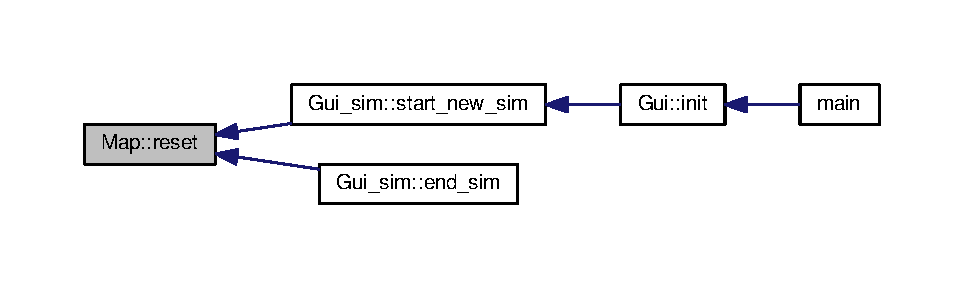
\includegraphics[width=350pt]{class_map_a904c445fdce79257fedeba09070cf88a_icgraph}
\end{center}
\end{figure}




\subsection{Member Data Documentation}
\hypertarget{class_map_a9fc5f65a162ff0459b3d23ba33b2b1e1}{\index{Map@{Map}!base\-\_\-res@{base\-\_\-res}}
\index{base\-\_\-res@{base\-\_\-res}!Map@{Map}}
\subsubsection[{base\-\_\-res}]{\setlength{\rightskip}{0pt plus 5cm}float$\ast$ Map\-::base\-\_\-res}}\label{class_map_a9fc5f65a162ff0459b3d23ba33b2b1e1}
\hypertarget{class_map_a72f5c51d7ba90727fcdff153b480c187}{\index{Map@{Map}!dangers@{dangers}}
\index{dangers@{dangers}!Map@{Map}}
\subsubsection[{dangers}]{\setlength{\rightskip}{0pt plus 5cm}float$\ast$$\ast$ Map\-::dangers}}\label{class_map_a72f5c51d7ba90727fcdff153b480c187}
\hypertarget{class_map_a496e559b2c5898e1622c962e6aa5e070}{\index{Map@{Map}!flags@{flags}}
\index{flags@{flags}!Map@{Map}}
\subsubsection[{flags}]{\setlength{\rightskip}{0pt plus 5cm}bool$\ast$$\ast$ Map\-::flags}}\label{class_map_a496e559b2c5898e1622c962e6aa5e070}
\hypertarget{class_map_a49a8163af842ed1d63f5d3d842f43c89}{\index{Map@{Map}!resources\-\_\-g@{resources\-\_\-g}}
\index{resources\-\_\-g@{resources\-\_\-g}!Map@{Map}}
\subsubsection[{resources\-\_\-g}]{\setlength{\rightskip}{0pt plus 5cm}float$\ast$$\ast$ Map\-::resources\-\_\-g}}\label{class_map_a49a8163af842ed1d63f5d3d842f43c89}
\hypertarget{class_map_a12ce9d7050191ba2f084e7e11cc41ab5}{\index{Map@{Map}!resources\-\_\-i@{resources\-\_\-i}}
\index{resources\-\_\-i@{resources\-\_\-i}!Map@{Map}}
\subsubsection[{resources\-\_\-i}]{\setlength{\rightskip}{0pt plus 5cm}float$\ast$$\ast$ Map\-::resources\-\_\-i}}\label{class_map_a12ce9d7050191ba2f084e7e11cc41ab5}
\hypertarget{class_map_a910f29ebb50c629a05c0945eb6c785ea}{\index{Map@{Map}!resources\-\_\-p@{resources\-\_\-p}}
\index{resources\-\_\-p@{resources\-\_\-p}!Map@{Map}}
\subsubsection[{resources\-\_\-p}]{\setlength{\rightskip}{0pt plus 5cm}float$\ast$$\ast$ Map\-::resources\-\_\-p}}\label{class_map_a910f29ebb50c629a05c0945eb6c785ea}


The documentation for this class was generated from the following files\-:\begin{DoxyCompactItemize}
\item 
/home/baios/\-Desktop/robsim/\-Rob\-Sim/include/backend/\hyperlink{_map_8h}{Map.\-h}\item 
/home/baios/\-Desktop/robsim/\-Rob\-Sim/src/backend/\hyperlink{_map_8cpp}{Map.\-cpp}\end{DoxyCompactItemize}

\hypertarget{class_probability}{\section{Probability Class Reference}
\label{class_probability}\index{Probability@{Probability}}
}


{\ttfamily \#include $<$Probability.\-h$>$}

\subsection*{Public Member Functions}
\begin{DoxyCompactItemize}
\item 
int \hyperlink{class_probability_af53f1705884b7d1b1fd658e3b525ee38}{take\-Damage} (\hyperlink{class_vehicle}{Vehicle} $\ast$v, float danger)
\item 
int \hyperlink{class_probability_a0b44decdf9ef28f67efe11f4c524c3e9}{take\-Damage} (\hyperlink{class_rescue_robot}{Rescue\-Robot} \&r, float danger)
\item 
int \hyperlink{class_probability_a5d26526a9d2ab3641e1ffe735f19c74a}{take\-Damage} (\hyperlink{class_research_robot}{Research\-Robot} \&s, float danger)
\item 
float \hyperlink{class_probability_a06a7e084593bdffb6a2a606f171cc49e}{calc\-\_\-probability} (float ability, float danger)
\end{DoxyCompactItemize}


\subsection{Member Function Documentation}
\hypertarget{class_probability_a06a7e084593bdffb6a2a606f171cc49e}{\index{Probability@{Probability}!calc\-\_\-probability@{calc\-\_\-probability}}
\index{calc\-\_\-probability@{calc\-\_\-probability}!Probability@{Probability}}
\subsubsection[{calc\-\_\-probability}]{\setlength{\rightskip}{0pt plus 5cm}float Probability\-::calc\-\_\-probability (
\begin{DoxyParamCaption}
\item[{float}]{ability, }
\item[{float}]{danger}
\end{DoxyParamCaption}
)}}\label{class_probability_a06a7e084593bdffb6a2a606f171cc49e}


Here is the caller graph for this function\-:
\nopagebreak
\begin{figure}[H]
\begin{center}
\leavevmode
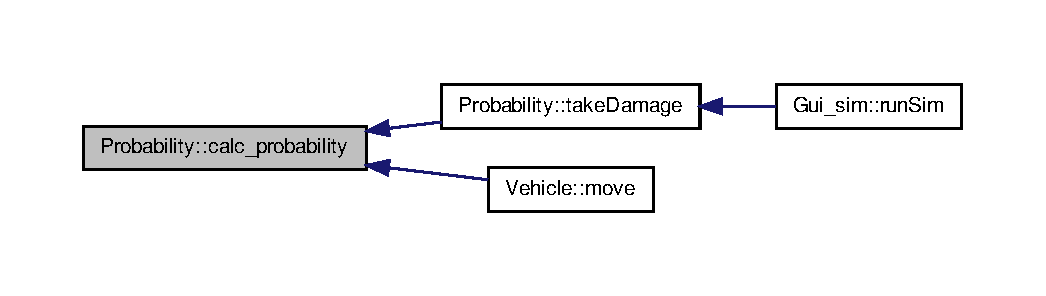
\includegraphics[width=350pt]{class_probability_a06a7e084593bdffb6a2a606f171cc49e_icgraph}
\end{center}
\end{figure}


\hypertarget{class_probability_af53f1705884b7d1b1fd658e3b525ee38}{\index{Probability@{Probability}!take\-Damage@{take\-Damage}}
\index{take\-Damage@{take\-Damage}!Probability@{Probability}}
\subsubsection[{take\-Damage}]{\setlength{\rightskip}{0pt plus 5cm}int Probability\-::take\-Damage (
\begin{DoxyParamCaption}
\item[{{\bf Vehicle} $\ast$}]{v, }
\item[{float}]{danger}
\end{DoxyParamCaption}
)}}\label{class_probability_af53f1705884b7d1b1fd658e3b525ee38}


Here is the call graph for this function\-:
\nopagebreak
\begin{figure}[H]
\begin{center}
\leavevmode
\includegraphics[width=350pt]{class_probability_af53f1705884b7d1b1fd658e3b525ee38_cgraph}
\end{center}
\end{figure}




Here is the caller graph for this function\-:
\nopagebreak
\begin{figure}[H]
\begin{center}
\leavevmode
\includegraphics[width=330pt]{class_probability_af53f1705884b7d1b1fd658e3b525ee38_icgraph}
\end{center}
\end{figure}


\hypertarget{class_probability_a0b44decdf9ef28f67efe11f4c524c3e9}{\index{Probability@{Probability}!take\-Damage@{take\-Damage}}
\index{take\-Damage@{take\-Damage}!Probability@{Probability}}
\subsubsection[{take\-Damage}]{\setlength{\rightskip}{0pt plus 5cm}int Probability\-::take\-Damage (
\begin{DoxyParamCaption}
\item[{{\bf Rescue\-Robot} \&}]{r, }
\item[{float}]{danger}
\end{DoxyParamCaption}
)}}\label{class_probability_a0b44decdf9ef28f67efe11f4c524c3e9}
\hypertarget{class_probability_a5d26526a9d2ab3641e1ffe735f19c74a}{\index{Probability@{Probability}!take\-Damage@{take\-Damage}}
\index{take\-Damage@{take\-Damage}!Probability@{Probability}}
\subsubsection[{take\-Damage}]{\setlength{\rightskip}{0pt plus 5cm}int Probability\-::take\-Damage (
\begin{DoxyParamCaption}
\item[{{\bf Research\-Robot} \&}]{s, }
\item[{float}]{danger}
\end{DoxyParamCaption}
)}}\label{class_probability_a5d26526a9d2ab3641e1ffe735f19c74a}


The documentation for this class was generated from the following files\-:\begin{DoxyCompactItemize}
\item 
/home/baios/\-Desktop/robsim/\-Rob\-Sim/include/backend/\hyperlink{_probability_8h}{Probability.\-h}\item 
/home/baios/\-Desktop/robsim/\-Rob\-Sim/src/backend/\hyperlink{_probability_8cpp}{Probability.\-cpp}\end{DoxyCompactItemize}

\hypertarget{class_random}{\section{Random Class Reference}
\label{class_random}\index{Random@{Random}}
}


{\ttfamily \#include $<$Random.\-h$>$}

\subsection*{Public Member Functions}
\begin{DoxyCompactItemize}
\item 
\hyperlink{class_random_acb76b49c3903a3c4fb67fd216341f08d}{Random} ()
\item 
int \hyperlink{class_random_a1b32c687f8635d039762a3622221a51c}{random\-\_\-int} (int limit)
\item 
float \hyperlink{class_random_a2687695605d92ffe2e3a7b0b9a072426}{random\-\_\-float} (int limit)
\item 
float \hyperlink{class_random_aded9aa728d247e3a8bdc86b89db1c303}{random\-\_\-0\-\_\-to\-\_\-1} ()
\item 
float \hyperlink{class_random_ab802a0d33e2137744baa721539d513a7}{random\-\_\-0\-\_\-to\-\_\-1} (float offset)
\end{DoxyCompactItemize}


\subsection{Constructor \& Destructor Documentation}
\hypertarget{class_random_acb76b49c3903a3c4fb67fd216341f08d}{\index{Random@{Random}!Random@{Random}}
\index{Random@{Random}!Random@{Random}}
\subsubsection[{Random}]{\setlength{\rightskip}{0pt plus 5cm}Random\-::\-Random (
\begin{DoxyParamCaption}
{}
\end{DoxyParamCaption}
)}}\label{class_random_acb76b49c3903a3c4fb67fd216341f08d}


\subsection{Member Function Documentation}
\hypertarget{class_random_aded9aa728d247e3a8bdc86b89db1c303}{\index{Random@{Random}!random\-\_\-0\-\_\-to\-\_\-1@{random\-\_\-0\-\_\-to\-\_\-1}}
\index{random\-\_\-0\-\_\-to\-\_\-1@{random\-\_\-0\-\_\-to\-\_\-1}!Random@{Random}}
\subsubsection[{random\-\_\-0\-\_\-to\-\_\-1}]{\setlength{\rightskip}{0pt plus 5cm}float Random\-::random\-\_\-0\-\_\-to\-\_\-1 (
\begin{DoxyParamCaption}
{}
\end{DoxyParamCaption}
)}}\label{class_random_aded9aa728d247e3a8bdc86b89db1c303}


Here is the call graph for this function\-:
\nopagebreak
\begin{figure}[H]
\begin{center}
\leavevmode
\includegraphics[width=350pt]{class_random_aded9aa728d247e3a8bdc86b89db1c303_cgraph}
\end{center}
\end{figure}




Here is the caller graph for this function\-:
\nopagebreak
\begin{figure}[H]
\begin{center}
\leavevmode
\includegraphics[width=330pt]{class_random_aded9aa728d247e3a8bdc86b89db1c303_icgraph}
\end{center}
\end{figure}


\hypertarget{class_random_ab802a0d33e2137744baa721539d513a7}{\index{Random@{Random}!random\-\_\-0\-\_\-to\-\_\-1@{random\-\_\-0\-\_\-to\-\_\-1}}
\index{random\-\_\-0\-\_\-to\-\_\-1@{random\-\_\-0\-\_\-to\-\_\-1}!Random@{Random}}
\subsubsection[{random\-\_\-0\-\_\-to\-\_\-1}]{\setlength{\rightskip}{0pt plus 5cm}float Random\-::random\-\_\-0\-\_\-to\-\_\-1 (
\begin{DoxyParamCaption}
\item[{float}]{offset}
\end{DoxyParamCaption}
)}}\label{class_random_ab802a0d33e2137744baa721539d513a7}


Here is the call graph for this function\-:
\nopagebreak
\begin{figure}[H]
\begin{center}
\leavevmode
\includegraphics[width=350pt]{class_random_ab802a0d33e2137744baa721539d513a7_cgraph}
\end{center}
\end{figure}


\hypertarget{class_random_a2687695605d92ffe2e3a7b0b9a072426}{\index{Random@{Random}!random\-\_\-float@{random\-\_\-float}}
\index{random\-\_\-float@{random\-\_\-float}!Random@{Random}}
\subsubsection[{random\-\_\-float}]{\setlength{\rightskip}{0pt plus 5cm}float Random\-::random\-\_\-float (
\begin{DoxyParamCaption}
\item[{int}]{limit}
\end{DoxyParamCaption}
)}}\label{class_random_a2687695605d92ffe2e3a7b0b9a072426}
\hypertarget{class_random_a1b32c687f8635d039762a3622221a51c}{\index{Random@{Random}!random\-\_\-int@{random\-\_\-int}}
\index{random\-\_\-int@{random\-\_\-int}!Random@{Random}}
\subsubsection[{random\-\_\-int}]{\setlength{\rightskip}{0pt plus 5cm}int Random\-::random\-\_\-int (
\begin{DoxyParamCaption}
\item[{int}]{limit}
\end{DoxyParamCaption}
)}}\label{class_random_a1b32c687f8635d039762a3622221a51c}


Here is the caller graph for this function\-:
\nopagebreak
\begin{figure}[H]
\begin{center}
\leavevmode
\includegraphics[width=350pt]{class_random_a1b32c687f8635d039762a3622221a51c_icgraph}
\end{center}
\end{figure}




The documentation for this class was generated from the following files\-:\begin{DoxyCompactItemize}
\item 
/home/baios/\-Desktop/robsim/\-Rob\-Sim/include/backend/\hyperlink{_random_8h}{Random.\-h}\item 
/home/baios/\-Desktop/robsim/\-Rob\-Sim/src/backend/\hyperlink{_random_8cpp}{Random.\-cpp}\end{DoxyCompactItemize}

\hypertarget{class_rescue_robot}{\section{Rescue\-Robot Class Reference}
\label{class_rescue_robot}\index{Rescue\-Robot@{Rescue\-Robot}}
}


{\ttfamily \#include $<$Rescue\-Robot.\-h$>$}



Inheritance diagram for Rescue\-Robot\-:
\nopagebreak
\begin{figure}[H]
\begin{center}
\leavevmode
\includegraphics[width=156pt]{class_rescue_robot__inherit__graph}
\end{center}
\end{figure}


Collaboration diagram for Rescue\-Robot\-:
\nopagebreak
\begin{figure}[H]
\begin{center}
\leavevmode
\includegraphics[width=156pt]{class_rescue_robot__coll__graph}
\end{center}
\end{figure}
\subsection*{Public Member Functions}
\begin{DoxyCompactItemize}
\item 
\hyperlink{class_rescue_robot_a74d8804d8bd465c17913a47676a167a0}{Rescue\-Robot} (int id, const int width, const int height)
\item 
virtual void \hyperlink{class_rescue_robot_a59762f159a621047e2ffc0be0cf46c9d}{operate} (\hyperlink{class_map}{Map} \&m)
\item 
int \hyperlink{class_rescue_robot_acd09bdf36f773ae6545ab25c4f64e8bd}{get\-\_\-repaired} ()
\item 
bool \hyperlink{class_rescue_robot_afe5a654af62b7aba9b4fa3a261854eaa}{get\-\_\-repaired\-This\-Round} ()
\item 
virtual void \hyperlink{class_rescue_robot_accdc41d98e3135f050ea97b3879f60b3}{export\-\_\-info} (bool \&successful\-Operation)
\item 
virtual void \hyperlink{class_rescue_robot_a508cf4e62ace7b794d7d6ba01b916727}{export\-\_\-total\-\_\-info} (int \&total\-\_\-successfull\-Ops)
\end{DoxyCompactItemize}
\subsection*{Additional Inherited Members}


\subsection{Constructor \& Destructor Documentation}
\hypertarget{class_rescue_robot_a74d8804d8bd465c17913a47676a167a0}{\index{Rescue\-Robot@{Rescue\-Robot}!Rescue\-Robot@{Rescue\-Robot}}
\index{Rescue\-Robot@{Rescue\-Robot}!RescueRobot@{Rescue\-Robot}}
\subsubsection[{Rescue\-Robot}]{\setlength{\rightskip}{0pt plus 5cm}Rescue\-Robot\-::\-Rescue\-Robot (
\begin{DoxyParamCaption}
\item[{int}]{id, }
\item[{const int}]{width, }
\item[{const int}]{height}
\end{DoxyParamCaption}
)}}\label{class_rescue_robot_a74d8804d8bd465c17913a47676a167a0}


Here is the call graph for this function\-:
\nopagebreak
\begin{figure}[H]
\begin{center}
\leavevmode
\includegraphics[width=350pt]{class_rescue_robot_a74d8804d8bd465c17913a47676a167a0_cgraph}
\end{center}
\end{figure}




\subsection{Member Function Documentation}
\hypertarget{class_rescue_robot_accdc41d98e3135f050ea97b3879f60b3}{\index{Rescue\-Robot@{Rescue\-Robot}!export\-\_\-info@{export\-\_\-info}}
\index{export\-\_\-info@{export\-\_\-info}!RescueRobot@{Rescue\-Robot}}
\subsubsection[{export\-\_\-info}]{\setlength{\rightskip}{0pt plus 5cm}void Rescue\-Robot\-::export\-\_\-info (
\begin{DoxyParamCaption}
\item[{bool \&}]{successful\-Operation}
\end{DoxyParamCaption}
)\hspace{0.3cm}{\ttfamily [virtual]}}}\label{class_rescue_robot_accdc41d98e3135f050ea97b3879f60b3}


Reimplemented from \hyperlink{class_vehicle_a1bedb710e134005b37a2848b2c3c4851}{Vehicle}.



Here is the call graph for this function\-:
\nopagebreak
\begin{figure}[H]
\begin{center}
\leavevmode
\includegraphics[width=350pt]{class_rescue_robot_accdc41d98e3135f050ea97b3879f60b3_cgraph}
\end{center}
\end{figure}


\hypertarget{class_rescue_robot_a508cf4e62ace7b794d7d6ba01b916727}{\index{Rescue\-Robot@{Rescue\-Robot}!export\-\_\-total\-\_\-info@{export\-\_\-total\-\_\-info}}
\index{export\-\_\-total\-\_\-info@{export\-\_\-total\-\_\-info}!RescueRobot@{Rescue\-Robot}}
\subsubsection[{export\-\_\-total\-\_\-info}]{\setlength{\rightskip}{0pt plus 5cm}void Rescue\-Robot\-::export\-\_\-total\-\_\-info (
\begin{DoxyParamCaption}
\item[{int \&}]{total\-\_\-successfull\-Ops}
\end{DoxyParamCaption}
)\hspace{0.3cm}{\ttfamily [virtual]}}}\label{class_rescue_robot_a508cf4e62ace7b794d7d6ba01b916727}


Reimplemented from \hyperlink{class_vehicle_a6f7de2dcc1d9ce62c1da282757b345f6}{Vehicle}.

\hypertarget{class_rescue_robot_acd09bdf36f773ae6545ab25c4f64e8bd}{\index{Rescue\-Robot@{Rescue\-Robot}!get\-\_\-repaired@{get\-\_\-repaired}}
\index{get\-\_\-repaired@{get\-\_\-repaired}!RescueRobot@{Rescue\-Robot}}
\subsubsection[{get\-\_\-repaired}]{\setlength{\rightskip}{0pt plus 5cm}int Rescue\-Robot\-::get\-\_\-repaired (
\begin{DoxyParamCaption}
{}
\end{DoxyParamCaption}
)}}\label{class_rescue_robot_acd09bdf36f773ae6545ab25c4f64e8bd}
\hypertarget{class_rescue_robot_afe5a654af62b7aba9b4fa3a261854eaa}{\index{Rescue\-Robot@{Rescue\-Robot}!get\-\_\-repaired\-This\-Round@{get\-\_\-repaired\-This\-Round}}
\index{get\-\_\-repaired\-This\-Round@{get\-\_\-repaired\-This\-Round}!RescueRobot@{Rescue\-Robot}}
\subsubsection[{get\-\_\-repaired\-This\-Round}]{\setlength{\rightskip}{0pt plus 5cm}bool Rescue\-Robot\-::get\-\_\-repaired\-This\-Round (
\begin{DoxyParamCaption}
{}
\end{DoxyParamCaption}
)}}\label{class_rescue_robot_afe5a654af62b7aba9b4fa3a261854eaa}


Here is the caller graph for this function\-:
\nopagebreak
\begin{figure}[H]
\begin{center}
\leavevmode
\includegraphics[width=350pt]{class_rescue_robot_afe5a654af62b7aba9b4fa3a261854eaa_icgraph}
\end{center}
\end{figure}


\hypertarget{class_rescue_robot_a59762f159a621047e2ffc0be0cf46c9d}{\index{Rescue\-Robot@{Rescue\-Robot}!operate@{operate}}
\index{operate@{operate}!RescueRobot@{Rescue\-Robot}}
\subsubsection[{operate}]{\setlength{\rightskip}{0pt plus 5cm}void Rescue\-Robot\-::operate (
\begin{DoxyParamCaption}
\item[{{\bf Map} \&}]{m}
\end{DoxyParamCaption}
)\hspace{0.3cm}{\ttfamily [virtual]}}}\label{class_rescue_robot_a59762f159a621047e2ffc0be0cf46c9d}


Implements \hyperlink{class_vehicle_a6a0ed71ee9d4c569ee26961b213775db}{Vehicle}.



Here is the call graph for this function\-:
\nopagebreak
\begin{figure}[H]
\begin{center}
\leavevmode
\includegraphics[width=350pt]{class_rescue_robot_a59762f159a621047e2ffc0be0cf46c9d_cgraph}
\end{center}
\end{figure}




The documentation for this class was generated from the following files\-:\begin{DoxyCompactItemize}
\item 
/home/baios/\-Desktop/robsim/\-Rob\-Sim/include/backend/\hyperlink{_rescue_robot_8h}{Rescue\-Robot.\-h}\item 
/home/baios/\-Desktop/robsim/\-Rob\-Sim/src/backend/\hyperlink{_rescue_robot_8cpp}{Rescue\-Robot.\-cpp}\end{DoxyCompactItemize}

\hypertarget{class_research_robot}{\section{Research\-Robot Class Reference}
\label{class_research_robot}\index{Research\-Robot@{Research\-Robot}}
}


{\ttfamily \#include $<$Research\-Robot.\-h$>$}



Inheritance diagram for Research\-Robot\-:\nopagebreak
\begin{figure}[H]
\begin{center}
\leavevmode
\includegraphics[width=164pt]{class_research_robot__inherit__graph}
\end{center}
\end{figure}


Collaboration diagram for Research\-Robot\-:\nopagebreak
\begin{figure}[H]
\begin{center}
\leavevmode
\includegraphics[width=164pt]{class_research_robot__coll__graph}
\end{center}
\end{figure}
\subsection*{Public Member Functions}
\begin{DoxyCompactItemize}
\item 
\hyperlink{class_research_robot_a9a80e8a64a4b95b19e965761b4c33b17}{Research\-Robot} (int id, const int width, const int height)
\item 
virtual void \hyperlink{class_research_robot_a275cc9e973d7c2b28a0346d485905b08}{operate} (\hyperlink{class_map}{Map} \&m)
\item 
int \hyperlink{class_research_robot_ad31aa4e3683a5de10268a8a6f17e232c}{get\-\_\-flags\-Deployed} ()
\item 
bool \hyperlink{class_research_robot_a45a6730bd1836498be4dc1bdcd666140}{get\-\_\-flag\-Deployed\-This\-Round} ()
\item 
virtual void \hyperlink{class_research_robot_a550dbf010c584e09f4c8e4f27286675a}{export\-\_\-info} (bool \&succesful\-Operation)
\item 
virtual void \hyperlink{class_research_robot_ad95ed058516e5b5d7c48e23e9c0ab2a3}{export\-\_\-total\-\_\-info} (int \&total\-\_\-successfull\-Ops)
\end{DoxyCompactItemize}
\subsection*{Additional Inherited Members}


\subsection{Constructor \& Destructor Documentation}
\hypertarget{class_research_robot_a9a80e8a64a4b95b19e965761b4c33b17}{\index{Research\-Robot@{Research\-Robot}!Research\-Robot@{Research\-Robot}}
\index{Research\-Robot@{Research\-Robot}!ResearchRobot@{Research\-Robot}}
\subsubsection[{Research\-Robot}]{\setlength{\rightskip}{0pt plus 5cm}Research\-Robot\-::\-Research\-Robot (
\begin{DoxyParamCaption}
\item[{int}]{id, }
\item[{const int}]{width, }
\item[{const int}]{height}
\end{DoxyParamCaption}
)}}\label{class_research_robot_a9a80e8a64a4b95b19e965761b4c33b17}


Here is the call graph for this function\-:\nopagebreak
\begin{figure}[H]
\begin{center}
\leavevmode
\includegraphics[width=350pt]{class_research_robot_a9a80e8a64a4b95b19e965761b4c33b17_cgraph}
\end{center}
\end{figure}




\subsection{Member Function Documentation}
\hypertarget{class_research_robot_a550dbf010c584e09f4c8e4f27286675a}{\index{Research\-Robot@{Research\-Robot}!export\-\_\-info@{export\-\_\-info}}
\index{export\-\_\-info@{export\-\_\-info}!ResearchRobot@{Research\-Robot}}
\subsubsection[{export\-\_\-info}]{\setlength{\rightskip}{0pt plus 5cm}void Research\-Robot\-::export\-\_\-info (
\begin{DoxyParamCaption}
\item[{bool \&}]{succesful\-Operation}
\end{DoxyParamCaption}
)\hspace{0.3cm}{\ttfamily [virtual]}}}\label{class_research_robot_a550dbf010c584e09f4c8e4f27286675a}


Reimplemented from \hyperlink{class_vehicle_a1bedb710e134005b37a2848b2c3c4851}{Vehicle}.



Here is the call graph for this function\-:\nopagebreak
\begin{figure}[H]
\begin{center}
\leavevmode
\includegraphics[width=350pt]{class_research_robot_a550dbf010c584e09f4c8e4f27286675a_cgraph}
\end{center}
\end{figure}


\hypertarget{class_research_robot_ad95ed058516e5b5d7c48e23e9c0ab2a3}{\index{Research\-Robot@{Research\-Robot}!export\-\_\-total\-\_\-info@{export\-\_\-total\-\_\-info}}
\index{export\-\_\-total\-\_\-info@{export\-\_\-total\-\_\-info}!ResearchRobot@{Research\-Robot}}
\subsubsection[{export\-\_\-total\-\_\-info}]{\setlength{\rightskip}{0pt plus 5cm}void Research\-Robot\-::export\-\_\-total\-\_\-info (
\begin{DoxyParamCaption}
\item[{int \&}]{total\-\_\-successfull\-Ops}
\end{DoxyParamCaption}
)\hspace{0.3cm}{\ttfamily [virtual]}}}\label{class_research_robot_ad95ed058516e5b5d7c48e23e9c0ab2a3}


Reimplemented from \hyperlink{class_vehicle_a6f7de2dcc1d9ce62c1da282757b345f6}{Vehicle}.

\hypertarget{class_research_robot_a45a6730bd1836498be4dc1bdcd666140}{\index{Research\-Robot@{Research\-Robot}!get\-\_\-flag\-Deployed\-This\-Round@{get\-\_\-flag\-Deployed\-This\-Round}}
\index{get\-\_\-flag\-Deployed\-This\-Round@{get\-\_\-flag\-Deployed\-This\-Round}!ResearchRobot@{Research\-Robot}}
\subsubsection[{get\-\_\-flag\-Deployed\-This\-Round}]{\setlength{\rightskip}{0pt plus 5cm}bool Research\-Robot\-::get\-\_\-flag\-Deployed\-This\-Round (
\begin{DoxyParamCaption}
{}
\end{DoxyParamCaption}
)}}\label{class_research_robot_a45a6730bd1836498be4dc1bdcd666140}


Here is the caller graph for this function\-:\nopagebreak
\begin{figure}[H]
\begin{center}
\leavevmode
\includegraphics[width=350pt]{class_research_robot_a45a6730bd1836498be4dc1bdcd666140_icgraph}
\end{center}
\end{figure}


\hypertarget{class_research_robot_ad31aa4e3683a5de10268a8a6f17e232c}{\index{Research\-Robot@{Research\-Robot}!get\-\_\-flags\-Deployed@{get\-\_\-flags\-Deployed}}
\index{get\-\_\-flags\-Deployed@{get\-\_\-flags\-Deployed}!ResearchRobot@{Research\-Robot}}
\subsubsection[{get\-\_\-flags\-Deployed}]{\setlength{\rightskip}{0pt plus 5cm}int Research\-Robot\-::get\-\_\-flags\-Deployed (
\begin{DoxyParamCaption}
{}
\end{DoxyParamCaption}
)}}\label{class_research_robot_ad31aa4e3683a5de10268a8a6f17e232c}
\hypertarget{class_research_robot_a275cc9e973d7c2b28a0346d485905b08}{\index{Research\-Robot@{Research\-Robot}!operate@{operate}}
\index{operate@{operate}!ResearchRobot@{Research\-Robot}}
\subsubsection[{operate}]{\setlength{\rightskip}{0pt plus 5cm}void Research\-Robot\-::operate (
\begin{DoxyParamCaption}
\item[{{\bf Map} \&}]{m}
\end{DoxyParamCaption}
)\hspace{0.3cm}{\ttfamily [virtual]}}}\label{class_research_robot_a275cc9e973d7c2b28a0346d485905b08}


Implements \hyperlink{class_vehicle_a6a0ed71ee9d4c569ee26961b213775db}{Vehicle}.



Here is the call graph for this function\-:\nopagebreak
\begin{figure}[H]
\begin{center}
\leavevmode
\includegraphics[width=350pt]{class_research_robot_a275cc9e973d7c2b28a0346d485905b08_cgraph}
\end{center}
\end{figure}




The documentation for this class was generated from the following files\-:\begin{DoxyCompactItemize}
\item 
/home/baios/\-Cpp\-\_\-\-Projects/\-Cpp\-Ceid/include/backend/\hyperlink{_research_robot_8h}{Research\-Robot.\-h}\item 
/home/baios/\-Cpp\-\_\-\-Projects/\-Cpp\-Ceid/src/backend/\hyperlink{_research_robot_8cpp}{Research\-Robot.\-cpp}\end{DoxyCompactItemize}

\hypertarget{class_robot__management}{\section{Robot\-\_\-management Class Reference}
\label{class_robot__management}\index{Robot\-\_\-management@{Robot\-\_\-management}}
}


{\ttfamily \#include $<$Robot\-\_\-management.\-h$>$}

\subsection*{Public Member Functions}
\begin{DoxyCompactItemize}
\item 
\hyperlink{class_robot__management_a7c70a0df4a26ead685202d372c756079}{Robot\-\_\-management} (const int width, const int height)
\item 
bool \hyperlink{class_robot__management_a9f55e341be1e0c8d5a532b63a31b5115}{check\-For\-Robots} (unsigned int x, unsigned int y)
\item 
bool \hyperlink{class_robot__management_afcf39f34f19143b28efa81af072a6159}{check\-For\-Robots} (unsigned int x, unsigned int y, int \&num, char \&type)
\item 
void \hyperlink{class_robot__management_a783299145c4194e2b005ec66b34026ee}{add\-Robot} (char type)
\item 
void \hyperlink{class_robot__management_afbd5514d1ae7869c50b41ed62ebedd42}{add\-Robot} (char type, int x, int y)
\item 
void \hyperlink{class_robot__management_aeda3aa818ca41a1825f40325aea1ca3c}{delete\-\_\-robot} (int id)
\item 
bool \hyperlink{class_robot__management_a6d7fc2f2442081b9cbf7ab62a60d5426}{list\-Empty} ()
\item 
void \hyperlink{class_robot__management_ac1a9ddc1089b1f4a26e7a7effef79142}{empty\-List} ()
\end{DoxyCompactItemize}
\subsection*{Static Public Attributes}
\begin{DoxyCompactItemize}
\item 
static std\-::vector$<$ \hyperlink{class_vehicle}{Vehicle} $\ast$ $>$ \hyperlink{class_robot__management_ac309bb3cf06c0a84b058bc1f0459de39}{roblist}
\end{DoxyCompactItemize}


\subsection{Constructor \& Destructor Documentation}
\hypertarget{class_robot__management_a7c70a0df4a26ead685202d372c756079}{\index{Robot\-\_\-management@{Robot\-\_\-management}!Robot\-\_\-management@{Robot\-\_\-management}}
\index{Robot\-\_\-management@{Robot\-\_\-management}!Robot_management@{Robot\-\_\-management}}
\subsubsection[{Robot\-\_\-management}]{\setlength{\rightskip}{0pt plus 5cm}Robot\-\_\-management\-::\-Robot\-\_\-management (
\begin{DoxyParamCaption}
\item[{const int}]{width, }
\item[{const int}]{height}
\end{DoxyParamCaption}
)}}\label{class_robot__management_a7c70a0df4a26ead685202d372c756079}


\subsection{Member Function Documentation}
\hypertarget{class_robot__management_a783299145c4194e2b005ec66b34026ee}{\index{Robot\-\_\-management@{Robot\-\_\-management}!add\-Robot@{add\-Robot}}
\index{add\-Robot@{add\-Robot}!Robot_management@{Robot\-\_\-management}}
\subsubsection[{add\-Robot}]{\setlength{\rightskip}{0pt plus 5cm}void Robot\-\_\-management\-::add\-Robot (
\begin{DoxyParamCaption}
\item[{char}]{type}
\end{DoxyParamCaption}
)}}\label{class_robot__management_a783299145c4194e2b005ec66b34026ee}


Here is the caller graph for this function\-:\nopagebreak
\begin{figure}[H]
\begin{center}
\leavevmode
\includegraphics[width=350pt]{class_robot__management_a783299145c4194e2b005ec66b34026ee_icgraph}
\end{center}
\end{figure}


\hypertarget{class_robot__management_afbd5514d1ae7869c50b41ed62ebedd42}{\index{Robot\-\_\-management@{Robot\-\_\-management}!add\-Robot@{add\-Robot}}
\index{add\-Robot@{add\-Robot}!Robot_management@{Robot\-\_\-management}}
\subsubsection[{add\-Robot}]{\setlength{\rightskip}{0pt plus 5cm}void Robot\-\_\-management\-::add\-Robot (
\begin{DoxyParamCaption}
\item[{char}]{type, }
\item[{int}]{x, }
\item[{int}]{y}
\end{DoxyParamCaption}
)}}\label{class_robot__management_afbd5514d1ae7869c50b41ed62ebedd42}
\hypertarget{class_robot__management_a9f55e341be1e0c8d5a532b63a31b5115}{\index{Robot\-\_\-management@{Robot\-\_\-management}!check\-For\-Robots@{check\-For\-Robots}}
\index{check\-For\-Robots@{check\-For\-Robots}!Robot_management@{Robot\-\_\-management}}
\subsubsection[{check\-For\-Robots}]{\setlength{\rightskip}{0pt plus 5cm}bool Robot\-\_\-management\-::check\-For\-Robots (
\begin{DoxyParamCaption}
\item[{unsigned int}]{x, }
\item[{unsigned int}]{y}
\end{DoxyParamCaption}
)}}\label{class_robot__management_a9f55e341be1e0c8d5a532b63a31b5115}


Here is the caller graph for this function\-:\nopagebreak
\begin{figure}[H]
\begin{center}
\leavevmode
\includegraphics[width=350pt]{class_robot__management_a9f55e341be1e0c8d5a532b63a31b5115_icgraph}
\end{center}
\end{figure}


\hypertarget{class_robot__management_afcf39f34f19143b28efa81af072a6159}{\index{Robot\-\_\-management@{Robot\-\_\-management}!check\-For\-Robots@{check\-For\-Robots}}
\index{check\-For\-Robots@{check\-For\-Robots}!Robot_management@{Robot\-\_\-management}}
\subsubsection[{check\-For\-Robots}]{\setlength{\rightskip}{0pt plus 5cm}bool Robot\-\_\-management\-::check\-For\-Robots (
\begin{DoxyParamCaption}
\item[{unsigned int}]{x, }
\item[{unsigned int}]{y, }
\item[{int \&}]{num, }
\item[{char \&}]{type}
\end{DoxyParamCaption}
)}}\label{class_robot__management_afcf39f34f19143b28efa81af072a6159}
\hypertarget{class_robot__management_aeda3aa818ca41a1825f40325aea1ca3c}{\index{Robot\-\_\-management@{Robot\-\_\-management}!delete\-\_\-robot@{delete\-\_\-robot}}
\index{delete\-\_\-robot@{delete\-\_\-robot}!Robot_management@{Robot\-\_\-management}}
\subsubsection[{delete\-\_\-robot}]{\setlength{\rightskip}{0pt plus 5cm}void Robot\-\_\-management\-::delete\-\_\-robot (
\begin{DoxyParamCaption}
\item[{int}]{id}
\end{DoxyParamCaption}
)}}\label{class_robot__management_aeda3aa818ca41a1825f40325aea1ca3c}


Here is the caller graph for this function\-:\nopagebreak
\begin{figure}[H]
\begin{center}
\leavevmode
\includegraphics[width=350pt]{class_robot__management_aeda3aa818ca41a1825f40325aea1ca3c_icgraph}
\end{center}
\end{figure}


\hypertarget{class_robot__management_ac1a9ddc1089b1f4a26e7a7effef79142}{\index{Robot\-\_\-management@{Robot\-\_\-management}!empty\-List@{empty\-List}}
\index{empty\-List@{empty\-List}!Robot_management@{Robot\-\_\-management}}
\subsubsection[{empty\-List}]{\setlength{\rightskip}{0pt plus 5cm}void Robot\-\_\-management\-::empty\-List (
\begin{DoxyParamCaption}
{}
\end{DoxyParamCaption}
)}}\label{class_robot__management_ac1a9ddc1089b1f4a26e7a7effef79142}


Here is the caller graph for this function\-:\nopagebreak
\begin{figure}[H]
\begin{center}
\leavevmode
\includegraphics[width=350pt]{class_robot__management_ac1a9ddc1089b1f4a26e7a7effef79142_icgraph}
\end{center}
\end{figure}


\hypertarget{class_robot__management_a6d7fc2f2442081b9cbf7ab62a60d5426}{\index{Robot\-\_\-management@{Robot\-\_\-management}!list\-Empty@{list\-Empty}}
\index{list\-Empty@{list\-Empty}!Robot_management@{Robot\-\_\-management}}
\subsubsection[{list\-Empty}]{\setlength{\rightskip}{0pt plus 5cm}bool Robot\-\_\-management\-::list\-Empty (
\begin{DoxyParamCaption}
{}
\end{DoxyParamCaption}
)}}\label{class_robot__management_a6d7fc2f2442081b9cbf7ab62a60d5426}


Here is the caller graph for this function\-:\nopagebreak
\begin{figure}[H]
\begin{center}
\leavevmode
\includegraphics[width=350pt]{class_robot__management_a6d7fc2f2442081b9cbf7ab62a60d5426_icgraph}
\end{center}
\end{figure}




\subsection{Member Data Documentation}
\hypertarget{class_robot__management_ac309bb3cf06c0a84b058bc1f0459de39}{\index{Robot\-\_\-management@{Robot\-\_\-management}!roblist@{roblist}}
\index{roblist@{roblist}!Robot_management@{Robot\-\_\-management}}
\subsubsection[{roblist}]{\setlength{\rightskip}{0pt plus 5cm}std\-::vector$<$ {\bf Vehicle} $\ast$ $>$ Robot\-\_\-management\-::roblist\hspace{0.3cm}{\ttfamily [static]}}}\label{class_robot__management_ac309bb3cf06c0a84b058bc1f0459de39}


The documentation for this class was generated from the following files\-:\begin{DoxyCompactItemize}
\item 
/home/baios/\-Cpp\-\_\-\-Projects/\-Cpp\-Ceid/include/backend/\hyperlink{_robot__management_8h}{Robot\-\_\-management.\-h}\item 
/home/baios/\-Cpp\-\_\-\-Projects/\-Cpp\-Ceid/src/backend/\hyperlink{_robot__management_8cpp}{Robot\-\_\-management.\-cpp}\end{DoxyCompactItemize}

\hypertarget{class_simulation_status}{\section{Simulation\-Status Class Reference}
\label{class_simulation_status}\index{Simulation\-Status@{Simulation\-Status}}
}


{\ttfamily \#include $<$Simulation\-Status.\-h$>$}

\subsection*{Public Member Functions}
\begin{DoxyCompactItemize}
\item 
\hyperlink{class_simulation_status_a47ed684ecf3306fc32e4ad543d9e8983}{Simulation\-Status} ()
\item 
bool \hyperlink{class_simulation_status_a536b34bf815fc21ac19e47b3505f4fd8}{success} (\hyperlink{class_map}{Map} m)
\item 
bool \hyperlink{class_simulation_status_a5b08c84c0472d7ffb1b27e25527c44b8}{fail} ()
\item 
void \hyperlink{class_simulation_status_a36156ed7ab9de73a0de7b1fe47f3aa99}{set\-\_\-limit} (float nlim)
\end{DoxyCompactItemize}


\subsection{Constructor \& Destructor Documentation}
\hypertarget{class_simulation_status_a47ed684ecf3306fc32e4ad543d9e8983}{\index{Simulation\-Status@{Simulation\-Status}!Simulation\-Status@{Simulation\-Status}}
\index{Simulation\-Status@{Simulation\-Status}!SimulationStatus@{Simulation\-Status}}
\subsubsection[{Simulation\-Status}]{\setlength{\rightskip}{0pt plus 5cm}Simulation\-Status\-::\-Simulation\-Status (
\begin{DoxyParamCaption}
{}
\end{DoxyParamCaption}
)}}\label{class_simulation_status_a47ed684ecf3306fc32e4ad543d9e8983}


\subsection{Member Function Documentation}
\hypertarget{class_simulation_status_a5b08c84c0472d7ffb1b27e25527c44b8}{\index{Simulation\-Status@{Simulation\-Status}!fail@{fail}}
\index{fail@{fail}!SimulationStatus@{Simulation\-Status}}
\subsubsection[{fail}]{\setlength{\rightskip}{0pt plus 5cm}bool Simulation\-Status\-::fail (
\begin{DoxyParamCaption}
{}
\end{DoxyParamCaption}
)}}\label{class_simulation_status_a5b08c84c0472d7ffb1b27e25527c44b8}


Here is the caller graph for this function\-:\nopagebreak
\begin{figure}[H]
\begin{center}
\leavevmode
\includegraphics[width=316pt]{class_simulation_status_a5b08c84c0472d7ffb1b27e25527c44b8_icgraph}
\end{center}
\end{figure}


\hypertarget{class_simulation_status_a36156ed7ab9de73a0de7b1fe47f3aa99}{\index{Simulation\-Status@{Simulation\-Status}!set\-\_\-limit@{set\-\_\-limit}}
\index{set\-\_\-limit@{set\-\_\-limit}!SimulationStatus@{Simulation\-Status}}
\subsubsection[{set\-\_\-limit}]{\setlength{\rightskip}{0pt plus 5cm}void Simulation\-Status\-::set\-\_\-limit (
\begin{DoxyParamCaption}
\item[{float}]{nlim}
\end{DoxyParamCaption}
)}}\label{class_simulation_status_a36156ed7ab9de73a0de7b1fe47f3aa99}
\hypertarget{class_simulation_status_a536b34bf815fc21ac19e47b3505f4fd8}{\index{Simulation\-Status@{Simulation\-Status}!success@{success}}
\index{success@{success}!SimulationStatus@{Simulation\-Status}}
\subsubsection[{success}]{\setlength{\rightskip}{0pt plus 5cm}bool Simulation\-Status\-::success (
\begin{DoxyParamCaption}
\item[{{\bf Map}}]{m}
\end{DoxyParamCaption}
)}}\label{class_simulation_status_a536b34bf815fc21ac19e47b3505f4fd8}


Here is the call graph for this function\-:\nopagebreak
\begin{figure}[H]
\begin{center}
\leavevmode
\includegraphics[width=336pt]{class_simulation_status_a536b34bf815fc21ac19e47b3505f4fd8_cgraph}
\end{center}
\end{figure}




Here is the caller graph for this function\-:\nopagebreak
\begin{figure}[H]
\begin{center}
\leavevmode
\includegraphics[width=340pt]{class_simulation_status_a536b34bf815fc21ac19e47b3505f4fd8_icgraph}
\end{center}
\end{figure}




The documentation for this class was generated from the following files\-:\begin{DoxyCompactItemize}
\item 
/home/baios/\-Cpp\-\_\-\-Projects/\-Cpp\-Ceid/include/backend/\hyperlink{_simulation_status_8h}{Simulation\-Status.\-h}\item 
/home/baios/\-Cpp\-\_\-\-Projects/\-Cpp\-Ceid/src/backend/\hyperlink{_simulation_status_8cpp}{Simulation\-Status.\-cpp}\end{DoxyCompactItemize}

\hypertarget{class_smart_base}{\section{Smart\-Base Class Reference}
\label{class_smart_base}\index{Smart\-Base@{Smart\-Base}}
}


{\ttfamily \#include $<$Smart\-Base.\-h$>$}

\subsection*{Public Member Functions}
\begin{DoxyCompactItemize}
\item 
\hyperlink{class_smart_base_acebd8654e2aba9939906a49330f446f1}{Smart\-Base} (\hyperlink{class_map}{Map} m)
\item 
void \hyperlink{class_smart_base_a20632e4931f3986878bb89ca36bdb1bb}{get\-\_\-needs} (float \&p, float \&g, float \&i)
\item 
void \hyperlink{class_smart_base_a9703c903bcbe39227f6d852b944543f4}{calc\-\_\-exact\-\_\-needs} (int x, int y, float rem\-\_\-load, float \&p, float \&g, float \&i)
\end{DoxyCompactItemize}


\subsection{Constructor \& Destructor Documentation}
\hypertarget{class_smart_base_acebd8654e2aba9939906a49330f446f1}{\index{Smart\-Base@{Smart\-Base}!Smart\-Base@{Smart\-Base}}
\index{Smart\-Base@{Smart\-Base}!SmartBase@{Smart\-Base}}
\subsubsection[{Smart\-Base}]{\setlength{\rightskip}{0pt plus 5cm}Smart\-Base\-::\-Smart\-Base (
\begin{DoxyParamCaption}
\item[{{\bf Map}}]{m}
\end{DoxyParamCaption}
)}}\label{class_smart_base_acebd8654e2aba9939906a49330f446f1}


\subsection{Member Function Documentation}
\hypertarget{class_smart_base_a9703c903bcbe39227f6d852b944543f4}{\index{Smart\-Base@{Smart\-Base}!calc\-\_\-exact\-\_\-needs@{calc\-\_\-exact\-\_\-needs}}
\index{calc\-\_\-exact\-\_\-needs@{calc\-\_\-exact\-\_\-needs}!SmartBase@{Smart\-Base}}
\subsubsection[{calc\-\_\-exact\-\_\-needs}]{\setlength{\rightskip}{0pt plus 5cm}void Smart\-Base\-::calc\-\_\-exact\-\_\-needs (
\begin{DoxyParamCaption}
\item[{int}]{x, }
\item[{int}]{y, }
\item[{float}]{rem\-\_\-load, }
\item[{float \&}]{p, }
\item[{float \&}]{g, }
\item[{float \&}]{i}
\end{DoxyParamCaption}
)}}\label{class_smart_base_a9703c903bcbe39227f6d852b944543f4}


Here is the caller graph for this function\-:\nopagebreak
\begin{figure}[H]
\begin{center}
\leavevmode
\includegraphics[width=350pt]{class_smart_base_a9703c903bcbe39227f6d852b944543f4_icgraph}
\end{center}
\end{figure}


\hypertarget{class_smart_base_a20632e4931f3986878bb89ca36bdb1bb}{\index{Smart\-Base@{Smart\-Base}!get\-\_\-needs@{get\-\_\-needs}}
\index{get\-\_\-needs@{get\-\_\-needs}!SmartBase@{Smart\-Base}}
\subsubsection[{get\-\_\-needs}]{\setlength{\rightskip}{0pt plus 5cm}void Smart\-Base\-::get\-\_\-needs (
\begin{DoxyParamCaption}
\item[{float \&}]{p, }
\item[{float \&}]{g, }
\item[{float \&}]{i}
\end{DoxyParamCaption}
)}}\label{class_smart_base_a20632e4931f3986878bb89ca36bdb1bb}


The documentation for this class was generated from the following files\-:\begin{DoxyCompactItemize}
\item 
/home/baios/\-Cpp\-\_\-\-Projects/\-Cpp\-Ceid/include/backend/\hyperlink{_smart_base_8h}{Smart\-Base.\-h}\item 
/home/baios/\-Cpp\-\_\-\-Projects/\-Cpp\-Ceid/src/backend/\hyperlink{_smart_base_8cpp}{Smart\-Base.\-cpp}\end{DoxyCompactItemize}

\hypertarget{class_vehicle}{\section{Vehicle Class Reference}
\label{class_vehicle}\index{Vehicle@{Vehicle}}
}


{\ttfamily \#include $<$Vehicle.\-h$>$}



Inheritance diagram for Vehicle\-:
\nopagebreak
\begin{figure}[H]
\begin{center}
\leavevmode
\includegraphics[width=350pt]{class_vehicle__inherit__graph}
\end{center}
\end{figure}
\subsection*{Public Member Functions}
\begin{DoxyCompactItemize}
\item 
\hyperlink{class_vehicle_aef579c9dd3b44a77ceb3addd4fefc47b}{Vehicle} (const int width, const int height)
\item 
virtual \hyperlink{class_vehicle_a61ab140c755b8e0e824d54117cf4546f}{$\sim$\-Vehicle} ()
\item 
int \hyperlink{class_vehicle_a7e287f67c54968a70d46ce63a94e9c63}{move} (\hyperlink{class_map}{Map} m)
\item 
virtual void \hyperlink{class_vehicle_a6a0ed71ee9d4c569ee26961b213775db}{operate} (\hyperlink{class_map}{Map} \&m)=0
\item 
int \hyperlink{class_vehicle_a9528f57214d74276572e7b3858715b40}{get\-\_\-pos\-\_\-x} ()
\item 
int \hyperlink{class_vehicle_af1ffe0bf89d9cdc3f55033d73d8fb283}{get\-\_\-pos\-\_\-y} ()
\item 
int \hyperlink{class_vehicle_aa133cd93822aad408c811f89a3a0b273}{get\-\_\-velocity} ()
\item 
int \hyperlink{class_vehicle_a035e04c7cb7a2976b50f816af49dfa9d}{get\-\_\-status} ()
\item 
int \hyperlink{class_vehicle_a8b95156ffce6a2defece8cdda3405449}{get\-\_\-num\-\_\-id} ()
\item 
float \hyperlink{class_vehicle_a2ca803306acbd7f5876f6a22023470c2}{get\-\_\-ability} ()
\item 
char \hyperlink{class_vehicle_a3957f26debbf0726bf983d70ebd9b334}{get\-\_\-type} ()
\item 
int \hyperlink{class_vehicle_a44cdd7a765e0ecc93cd88c4449c7ff2a}{get\-\_\-travelled} ()
\item 
bool \hyperlink{class_vehicle_ada86b9d1054e3841d3fb0d5433e11774}{get\-\_\-broke\-Q} ()
\item 
void \hyperlink{class_vehicle_a933de97259d52a073e167cb4902cf272}{set\-\_\-type} (char type)
\item 
void \hyperlink{class_vehicle_a33fa7c0df43c6f1de03339745ba226e7}{set\-\_\-num\-\_\-id} (int num)
\item 
void \hyperlink{class_vehicle_abebe961f59c383b6ae23c1eb9a011519}{set\-\_\-velocity} (int num)
\item 
void \hyperlink{class_vehicle_a5295b6b7ebd67c074896604d06f30b53}{set\-\_\-pos\-\_\-x} (int x)
\item 
void \hyperlink{class_vehicle_a91b3331fbf7fa63198b22ded702a6a44}{set\-\_\-pos\-\_\-y} (int y)
\item 
void \hyperlink{class_vehicle_ad2ab1a15c767bbdd09e1190a18f1bdca}{set\-\_\-ability} (float ab)
\item 
void \hyperlink{class_vehicle_a87b875939c76d2a2f984811f60dd2af4}{set\-\_\-status} (int n\-\_\-status)
\item 
void \hyperlink{class_vehicle_a32d6fb4b960170d7a88c9ba4cdf30710}{return\-To\-Map} ()
\item 
bool \hyperlink{class_vehicle_a7c78e8942102b824144cc227984ea988}{check\-Robot\-Death} ()
\item 
virtual void \hyperlink{class_vehicle_a3e3cc666c76c42178e942363585ff1b7}{export\-\_\-info} (float \&p, float \&g, float \&i, float \&rem\-Load)
\item 
virtual void \hyperlink{class_vehicle_a1bedb710e134005b37a2848b2c3c4851}{export\-\_\-info} (bool \&successful\-Operation)
\item 
virtual void \hyperlink{class_vehicle_ae2840b7627d758e5019a6fdd83a229a9}{export\-\_\-total\-\_\-info} (float \&tp, float \&tg, float \&ti, float \&total\-\_\-res)
\item 
virtual void \hyperlink{class_vehicle_a6f7de2dcc1d9ce62c1da282757b345f6}{export\-\_\-total\-\_\-info} (int \&total\-\_\-successfull\-Ops)
\end{DoxyCompactItemize}
\subsection*{Public Attributes}
\begin{DoxyCompactItemize}
\item 
bool \hyperlink{class_vehicle_a0130974e6ab67f6a2b59772b5de4cc6e}{goto\-Base}
\item 
int \hyperlink{class_vehicle_a8ec5bc4761c8ab8b17a69d9a9e8c5d2c}{def\-\_\-velocity}
\item 
int \hyperlink{class_vehicle_a18846d0cdc78a3f2137e70021af01492}{def\-\_\-status}
\item 
int \hyperlink{class_vehicle_a9ff49e3ecf77a8b92fb3d48ccd08dba3}{total\-\_\-damages}
\end{DoxyCompactItemize}


\subsection{Constructor \& Destructor Documentation}
\hypertarget{class_vehicle_aef579c9dd3b44a77ceb3addd4fefc47b}{\index{Vehicle@{Vehicle}!Vehicle@{Vehicle}}
\index{Vehicle@{Vehicle}!Vehicle@{Vehicle}}
\subsubsection[{Vehicle}]{\setlength{\rightskip}{0pt plus 5cm}Vehicle\-::\-Vehicle (
\begin{DoxyParamCaption}
\item[{const int}]{width, }
\item[{const int}]{height}
\end{DoxyParamCaption}
)}}\label{class_vehicle_aef579c9dd3b44a77ceb3addd4fefc47b}


Here is the call graph for this function\-:
\nopagebreak
\begin{figure}[H]
\begin{center}
\leavevmode
\includegraphics[width=350pt]{class_vehicle_aef579c9dd3b44a77ceb3addd4fefc47b_cgraph}
\end{center}
\end{figure}


\hypertarget{class_vehicle_a61ab140c755b8e0e824d54117cf4546f}{\index{Vehicle@{Vehicle}!$\sim$\-Vehicle@{$\sim$\-Vehicle}}
\index{$\sim$\-Vehicle@{$\sim$\-Vehicle}!Vehicle@{Vehicle}}
\subsubsection[{$\sim$\-Vehicle}]{\setlength{\rightskip}{0pt plus 5cm}Vehicle\-::$\sim$\-Vehicle (
\begin{DoxyParamCaption}
{}
\end{DoxyParamCaption}
)\hspace{0.3cm}{\ttfamily [virtual]}}}\label{class_vehicle_a61ab140c755b8e0e824d54117cf4546f}


\subsection{Member Function Documentation}
\hypertarget{class_vehicle_a7c78e8942102b824144cc227984ea988}{\index{Vehicle@{Vehicle}!check\-Robot\-Death@{check\-Robot\-Death}}
\index{check\-Robot\-Death@{check\-Robot\-Death}!Vehicle@{Vehicle}}
\subsubsection[{check\-Robot\-Death}]{\setlength{\rightskip}{0pt plus 5cm}bool Vehicle\-::check\-Robot\-Death (
\begin{DoxyParamCaption}
{}
\end{DoxyParamCaption}
)}}\label{class_vehicle_a7c78e8942102b824144cc227984ea988}


Here is the call graph for this function\-:
\nopagebreak
\begin{figure}[H]
\begin{center}
\leavevmode
\includegraphics[width=350pt]{class_vehicle_a7c78e8942102b824144cc227984ea988_cgraph}
\end{center}
\end{figure}




Here is the caller graph for this function\-:
\nopagebreak
\begin{figure}[H]
\begin{center}
\leavevmode
\includegraphics[width=350pt]{class_vehicle_a7c78e8942102b824144cc227984ea988_icgraph}
\end{center}
\end{figure}


\hypertarget{class_vehicle_a3e3cc666c76c42178e942363585ff1b7}{\index{Vehicle@{Vehicle}!export\-\_\-info@{export\-\_\-info}}
\index{export\-\_\-info@{export\-\_\-info}!Vehicle@{Vehicle}}
\subsubsection[{export\-\_\-info}]{\setlength{\rightskip}{0pt plus 5cm}void Vehicle\-::export\-\_\-info (
\begin{DoxyParamCaption}
\item[{float \&}]{p, }
\item[{float \&}]{g, }
\item[{float \&}]{i, }
\item[{float \&}]{rem\-Load}
\end{DoxyParamCaption}
)\hspace{0.3cm}{\ttfamily [virtual]}}}\label{class_vehicle_a3e3cc666c76c42178e942363585ff1b7}


Reimplemented in \hyperlink{class_analysis_robot_a984f9a02843c487538dcb8029f15ce1f}{Analysis\-Robot}.

\hypertarget{class_vehicle_a1bedb710e134005b37a2848b2c3c4851}{\index{Vehicle@{Vehicle}!export\-\_\-info@{export\-\_\-info}}
\index{export\-\_\-info@{export\-\_\-info}!Vehicle@{Vehicle}}
\subsubsection[{export\-\_\-info}]{\setlength{\rightskip}{0pt plus 5cm}void Vehicle\-::export\-\_\-info (
\begin{DoxyParamCaption}
\item[{bool \&}]{successful\-Operation}
\end{DoxyParamCaption}
)\hspace{0.3cm}{\ttfamily [virtual]}}}\label{class_vehicle_a1bedb710e134005b37a2848b2c3c4851}


Reimplemented in \hyperlink{class_research_robot_a550dbf010c584e09f4c8e4f27286675a}{Research\-Robot}, and \hyperlink{class_rescue_robot_accdc41d98e3135f050ea97b3879f60b3}{Rescue\-Robot}.

\hypertarget{class_vehicle_ae2840b7627d758e5019a6fdd83a229a9}{\index{Vehicle@{Vehicle}!export\-\_\-total\-\_\-info@{export\-\_\-total\-\_\-info}}
\index{export\-\_\-total\-\_\-info@{export\-\_\-total\-\_\-info}!Vehicle@{Vehicle}}
\subsubsection[{export\-\_\-total\-\_\-info}]{\setlength{\rightskip}{0pt plus 5cm}void Vehicle\-::export\-\_\-total\-\_\-info (
\begin{DoxyParamCaption}
\item[{float \&}]{tp, }
\item[{float \&}]{tg, }
\item[{float \&}]{ti, }
\item[{float \&}]{total\-\_\-res}
\end{DoxyParamCaption}
)\hspace{0.3cm}{\ttfamily [virtual]}}}\label{class_vehicle_ae2840b7627d758e5019a6fdd83a229a9}


Reimplemented in \hyperlink{class_analysis_robot_a090c8f17c57af7c3073905fa9bedbf2c}{Analysis\-Robot}.

\hypertarget{class_vehicle_a6f7de2dcc1d9ce62c1da282757b345f6}{\index{Vehicle@{Vehicle}!export\-\_\-total\-\_\-info@{export\-\_\-total\-\_\-info}}
\index{export\-\_\-total\-\_\-info@{export\-\_\-total\-\_\-info}!Vehicle@{Vehicle}}
\subsubsection[{export\-\_\-total\-\_\-info}]{\setlength{\rightskip}{0pt plus 5cm}void Vehicle\-::export\-\_\-total\-\_\-info (
\begin{DoxyParamCaption}
\item[{int \&}]{total\-\_\-successfull\-Ops}
\end{DoxyParamCaption}
)\hspace{0.3cm}{\ttfamily [virtual]}}}\label{class_vehicle_a6f7de2dcc1d9ce62c1da282757b345f6}


Reimplemented in \hyperlink{class_research_robot_ad95ed058516e5b5d7c48e23e9c0ab2a3}{Research\-Robot}, and \hyperlink{class_rescue_robot_a508cf4e62ace7b794d7d6ba01b916727}{Rescue\-Robot}.

\hypertarget{class_vehicle_a2ca803306acbd7f5876f6a22023470c2}{\index{Vehicle@{Vehicle}!get\-\_\-ability@{get\-\_\-ability}}
\index{get\-\_\-ability@{get\-\_\-ability}!Vehicle@{Vehicle}}
\subsubsection[{get\-\_\-ability}]{\setlength{\rightskip}{0pt plus 5cm}float Vehicle\-::get\-\_\-ability (
\begin{DoxyParamCaption}
{}
\end{DoxyParamCaption}
)}}\label{class_vehicle_a2ca803306acbd7f5876f6a22023470c2}


Here is the caller graph for this function\-:
\nopagebreak
\begin{figure}[H]
\begin{center}
\leavevmode
\includegraphics[width=350pt]{class_vehicle_a2ca803306acbd7f5876f6a22023470c2_icgraph}
\end{center}
\end{figure}


\hypertarget{class_vehicle_ada86b9d1054e3841d3fb0d5433e11774}{\index{Vehicle@{Vehicle}!get\-\_\-broke\-Q@{get\-\_\-broke\-Q}}
\index{get\-\_\-broke\-Q@{get\-\_\-broke\-Q}!Vehicle@{Vehicle}}
\subsubsection[{get\-\_\-broke\-Q}]{\setlength{\rightskip}{0pt plus 5cm}bool Vehicle\-::get\-\_\-broke\-Q (
\begin{DoxyParamCaption}
{}
\end{DoxyParamCaption}
)}}\label{class_vehicle_ada86b9d1054e3841d3fb0d5433e11774}
\hypertarget{class_vehicle_a8b95156ffce6a2defece8cdda3405449}{\index{Vehicle@{Vehicle}!get\-\_\-num\-\_\-id@{get\-\_\-num\-\_\-id}}
\index{get\-\_\-num\-\_\-id@{get\-\_\-num\-\_\-id}!Vehicle@{Vehicle}}
\subsubsection[{get\-\_\-num\-\_\-id}]{\setlength{\rightskip}{0pt plus 5cm}int Vehicle\-::get\-\_\-num\-\_\-id (
\begin{DoxyParamCaption}
{}
\end{DoxyParamCaption}
)}}\label{class_vehicle_a8b95156ffce6a2defece8cdda3405449}


Here is the caller graph for this function\-:
\nopagebreak
\begin{figure}[H]
\begin{center}
\leavevmode
\includegraphics[width=338pt]{class_vehicle_a8b95156ffce6a2defece8cdda3405449_icgraph}
\end{center}
\end{figure}


\hypertarget{class_vehicle_a9528f57214d74276572e7b3858715b40}{\index{Vehicle@{Vehicle}!get\-\_\-pos\-\_\-x@{get\-\_\-pos\-\_\-x}}
\index{get\-\_\-pos\-\_\-x@{get\-\_\-pos\-\_\-x}!Vehicle@{Vehicle}}
\subsubsection[{get\-\_\-pos\-\_\-x}]{\setlength{\rightskip}{0pt plus 5cm}int Vehicle\-::get\-\_\-pos\-\_\-x (
\begin{DoxyParamCaption}
{}
\end{DoxyParamCaption}
)}}\label{class_vehicle_a9528f57214d74276572e7b3858715b40}


Here is the caller graph for this function\-:
\nopagebreak
\begin{figure}[H]
\begin{center}
\leavevmode
\includegraphics[width=340pt]{class_vehicle_a9528f57214d74276572e7b3858715b40_icgraph}
\end{center}
\end{figure}


\hypertarget{class_vehicle_af1ffe0bf89d9cdc3f55033d73d8fb283}{\index{Vehicle@{Vehicle}!get\-\_\-pos\-\_\-y@{get\-\_\-pos\-\_\-y}}
\index{get\-\_\-pos\-\_\-y@{get\-\_\-pos\-\_\-y}!Vehicle@{Vehicle}}
\subsubsection[{get\-\_\-pos\-\_\-y}]{\setlength{\rightskip}{0pt plus 5cm}int Vehicle\-::get\-\_\-pos\-\_\-y (
\begin{DoxyParamCaption}
{}
\end{DoxyParamCaption}
)}}\label{class_vehicle_af1ffe0bf89d9cdc3f55033d73d8fb283}


Here is the caller graph for this function\-:
\nopagebreak
\begin{figure}[H]
\begin{center}
\leavevmode
\includegraphics[width=340pt]{class_vehicle_af1ffe0bf89d9cdc3f55033d73d8fb283_icgraph}
\end{center}
\end{figure}


\hypertarget{class_vehicle_a035e04c7cb7a2976b50f816af49dfa9d}{\index{Vehicle@{Vehicle}!get\-\_\-status@{get\-\_\-status}}
\index{get\-\_\-status@{get\-\_\-status}!Vehicle@{Vehicle}}
\subsubsection[{get\-\_\-status}]{\setlength{\rightskip}{0pt plus 5cm}int Vehicle\-::get\-\_\-status (
\begin{DoxyParamCaption}
{}
\end{DoxyParamCaption}
)}}\label{class_vehicle_a035e04c7cb7a2976b50f816af49dfa9d}


Here is the caller graph for this function\-:
\nopagebreak
\begin{figure}[H]
\begin{center}
\leavevmode
\includegraphics[width=350pt]{class_vehicle_a035e04c7cb7a2976b50f816af49dfa9d_icgraph}
\end{center}
\end{figure}


\hypertarget{class_vehicle_a44cdd7a765e0ecc93cd88c4449c7ff2a}{\index{Vehicle@{Vehicle}!get\-\_\-travelled@{get\-\_\-travelled}}
\index{get\-\_\-travelled@{get\-\_\-travelled}!Vehicle@{Vehicle}}
\subsubsection[{get\-\_\-travelled}]{\setlength{\rightskip}{0pt plus 5cm}int Vehicle\-::get\-\_\-travelled (
\begin{DoxyParamCaption}
{}
\end{DoxyParamCaption}
)}}\label{class_vehicle_a44cdd7a765e0ecc93cd88c4449c7ff2a}
\hypertarget{class_vehicle_a3957f26debbf0726bf983d70ebd9b334}{\index{Vehicle@{Vehicle}!get\-\_\-type@{get\-\_\-type}}
\index{get\-\_\-type@{get\-\_\-type}!Vehicle@{Vehicle}}
\subsubsection[{get\-\_\-type}]{\setlength{\rightskip}{0pt plus 5cm}char Vehicle\-::get\-\_\-type (
\begin{DoxyParamCaption}
{}
\end{DoxyParamCaption}
)}}\label{class_vehicle_a3957f26debbf0726bf983d70ebd9b334}


Here is the caller graph for this function\-:
\nopagebreak
\begin{figure}[H]
\begin{center}
\leavevmode
\includegraphics[width=324pt]{class_vehicle_a3957f26debbf0726bf983d70ebd9b334_icgraph}
\end{center}
\end{figure}


\hypertarget{class_vehicle_aa133cd93822aad408c811f89a3a0b273}{\index{Vehicle@{Vehicle}!get\-\_\-velocity@{get\-\_\-velocity}}
\index{get\-\_\-velocity@{get\-\_\-velocity}!Vehicle@{Vehicle}}
\subsubsection[{get\-\_\-velocity}]{\setlength{\rightskip}{0pt plus 5cm}int Vehicle\-::get\-\_\-velocity (
\begin{DoxyParamCaption}
{}
\end{DoxyParamCaption}
)}}\label{class_vehicle_aa133cd93822aad408c811f89a3a0b273}
\hypertarget{class_vehicle_a7e287f67c54968a70d46ce63a94e9c63}{\index{Vehicle@{Vehicle}!move@{move}}
\index{move@{move}!Vehicle@{Vehicle}}
\subsubsection[{move}]{\setlength{\rightskip}{0pt plus 5cm}int Vehicle\-::move (
\begin{DoxyParamCaption}
\item[{{\bf Map}}]{m}
\end{DoxyParamCaption}
)}}\label{class_vehicle_a7e287f67c54968a70d46ce63a94e9c63}


Here is the call graph for this function\-:
\nopagebreak
\begin{figure}[H]
\begin{center}
\leavevmode
\includegraphics[width=350pt]{class_vehicle_a7e287f67c54968a70d46ce63a94e9c63_cgraph}
\end{center}
\end{figure}


\hypertarget{class_vehicle_a6a0ed71ee9d4c569ee26961b213775db}{\index{Vehicle@{Vehicle}!operate@{operate}}
\index{operate@{operate}!Vehicle@{Vehicle}}
\subsubsection[{operate}]{\setlength{\rightskip}{0pt plus 5cm}virtual void Vehicle\-::operate (
\begin{DoxyParamCaption}
\item[{{\bf Map} \&}]{m}
\end{DoxyParamCaption}
)\hspace{0.3cm}{\ttfamily [pure virtual]}}}\label{class_vehicle_a6a0ed71ee9d4c569ee26961b213775db}


Implemented in \hyperlink{class_research_robot_a275cc9e973d7c2b28a0346d485905b08}{Research\-Robot}, \hyperlink{class_analysis_robot_a496ce06a9eee3fcbb521dd6eb9ef7947}{Analysis\-Robot}, and \hyperlink{class_rescue_robot_a59762f159a621047e2ffc0be0cf46c9d}{Rescue\-Robot}.

\hypertarget{class_vehicle_a32d6fb4b960170d7a88c9ba4cdf30710}{\index{Vehicle@{Vehicle}!return\-To\-Map@{return\-To\-Map}}
\index{return\-To\-Map@{return\-To\-Map}!Vehicle@{Vehicle}}
\subsubsection[{return\-To\-Map}]{\setlength{\rightskip}{0pt plus 5cm}void Vehicle\-::return\-To\-Map (
\begin{DoxyParamCaption}
{}
\end{DoxyParamCaption}
)}}\label{class_vehicle_a32d6fb4b960170d7a88c9ba4cdf30710}


Here is the call graph for this function\-:
\nopagebreak
\begin{figure}[H]
\begin{center}
\leavevmode
\includegraphics[width=326pt]{class_vehicle_a32d6fb4b960170d7a88c9ba4cdf30710_cgraph}
\end{center}
\end{figure}




Here is the caller graph for this function\-:
\nopagebreak
\begin{figure}[H]
\begin{center}
\leavevmode
\includegraphics[width=346pt]{class_vehicle_a32d6fb4b960170d7a88c9ba4cdf30710_icgraph}
\end{center}
\end{figure}


\hypertarget{class_vehicle_ad2ab1a15c767bbdd09e1190a18f1bdca}{\index{Vehicle@{Vehicle}!set\-\_\-ability@{set\-\_\-ability}}
\index{set\-\_\-ability@{set\-\_\-ability}!Vehicle@{Vehicle}}
\subsubsection[{set\-\_\-ability}]{\setlength{\rightskip}{0pt plus 5cm}void Vehicle\-::set\-\_\-ability (
\begin{DoxyParamCaption}
\item[{float}]{ab}
\end{DoxyParamCaption}
)}}\label{class_vehicle_ad2ab1a15c767bbdd09e1190a18f1bdca}
\hypertarget{class_vehicle_a33fa7c0df43c6f1de03339745ba226e7}{\index{Vehicle@{Vehicle}!set\-\_\-num\-\_\-id@{set\-\_\-num\-\_\-id}}
\index{set\-\_\-num\-\_\-id@{set\-\_\-num\-\_\-id}!Vehicle@{Vehicle}}
\subsubsection[{set\-\_\-num\-\_\-id}]{\setlength{\rightskip}{0pt plus 5cm}void Vehicle\-::set\-\_\-num\-\_\-id (
\begin{DoxyParamCaption}
\item[{int}]{num}
\end{DoxyParamCaption}
)}}\label{class_vehicle_a33fa7c0df43c6f1de03339745ba226e7}


Here is the caller graph for this function\-:
\nopagebreak
\begin{figure}[H]
\begin{center}
\leavevmode
\includegraphics[width=350pt]{class_vehicle_a33fa7c0df43c6f1de03339745ba226e7_icgraph}
\end{center}
\end{figure}


\hypertarget{class_vehicle_a5295b6b7ebd67c074896604d06f30b53}{\index{Vehicle@{Vehicle}!set\-\_\-pos\-\_\-x@{set\-\_\-pos\-\_\-x}}
\index{set\-\_\-pos\-\_\-x@{set\-\_\-pos\-\_\-x}!Vehicle@{Vehicle}}
\subsubsection[{set\-\_\-pos\-\_\-x}]{\setlength{\rightskip}{0pt plus 5cm}void Vehicle\-::set\-\_\-pos\-\_\-x (
\begin{DoxyParamCaption}
\item[{int}]{x}
\end{DoxyParamCaption}
)}}\label{class_vehicle_a5295b6b7ebd67c074896604d06f30b53}


Here is the caller graph for this function\-:
\nopagebreak
\begin{figure}[H]
\begin{center}
\leavevmode
\includegraphics[width=350pt]{class_vehicle_a5295b6b7ebd67c074896604d06f30b53_icgraph}
\end{center}
\end{figure}


\hypertarget{class_vehicle_a91b3331fbf7fa63198b22ded702a6a44}{\index{Vehicle@{Vehicle}!set\-\_\-pos\-\_\-y@{set\-\_\-pos\-\_\-y}}
\index{set\-\_\-pos\-\_\-y@{set\-\_\-pos\-\_\-y}!Vehicle@{Vehicle}}
\subsubsection[{set\-\_\-pos\-\_\-y}]{\setlength{\rightskip}{0pt plus 5cm}void Vehicle\-::set\-\_\-pos\-\_\-y (
\begin{DoxyParamCaption}
\item[{int}]{y}
\end{DoxyParamCaption}
)}}\label{class_vehicle_a91b3331fbf7fa63198b22ded702a6a44}


Here is the caller graph for this function\-:
\nopagebreak
\begin{figure}[H]
\begin{center}
\leavevmode
\includegraphics[width=350pt]{class_vehicle_a91b3331fbf7fa63198b22ded702a6a44_icgraph}
\end{center}
\end{figure}


\hypertarget{class_vehicle_a87b875939c76d2a2f984811f60dd2af4}{\index{Vehicle@{Vehicle}!set\-\_\-status@{set\-\_\-status}}
\index{set\-\_\-status@{set\-\_\-status}!Vehicle@{Vehicle}}
\subsubsection[{set\-\_\-status}]{\setlength{\rightskip}{0pt plus 5cm}void Vehicle\-::set\-\_\-status (
\begin{DoxyParamCaption}
\item[{int}]{n\-\_\-status}
\end{DoxyParamCaption}
)}}\label{class_vehicle_a87b875939c76d2a2f984811f60dd2af4}


Here is the call graph for this function\-:
\nopagebreak
\begin{figure}[H]
\begin{center}
\leavevmode
\includegraphics[width=326pt]{class_vehicle_a87b875939c76d2a2f984811f60dd2af4_cgraph}
\end{center}
\end{figure}




Here is the caller graph for this function\-:
\nopagebreak
\begin{figure}[H]
\begin{center}
\leavevmode
\includegraphics[width=350pt]{class_vehicle_a87b875939c76d2a2f984811f60dd2af4_icgraph}
\end{center}
\end{figure}


\hypertarget{class_vehicle_a933de97259d52a073e167cb4902cf272}{\index{Vehicle@{Vehicle}!set\-\_\-type@{set\-\_\-type}}
\index{set\-\_\-type@{set\-\_\-type}!Vehicle@{Vehicle}}
\subsubsection[{set\-\_\-type}]{\setlength{\rightskip}{0pt plus 5cm}void Vehicle\-::set\-\_\-type (
\begin{DoxyParamCaption}
\item[{char}]{type}
\end{DoxyParamCaption}
)}}\label{class_vehicle_a933de97259d52a073e167cb4902cf272}


Here is the caller graph for this function\-:
\nopagebreak
\begin{figure}[H]
\begin{center}
\leavevmode
\includegraphics[width=350pt]{class_vehicle_a933de97259d52a073e167cb4902cf272_icgraph}
\end{center}
\end{figure}


\hypertarget{class_vehicle_abebe961f59c383b6ae23c1eb9a011519}{\index{Vehicle@{Vehicle}!set\-\_\-velocity@{set\-\_\-velocity}}
\index{set\-\_\-velocity@{set\-\_\-velocity}!Vehicle@{Vehicle}}
\subsubsection[{set\-\_\-velocity}]{\setlength{\rightskip}{0pt plus 5cm}void Vehicle\-::set\-\_\-velocity (
\begin{DoxyParamCaption}
\item[{int}]{num}
\end{DoxyParamCaption}
)}}\label{class_vehicle_abebe961f59c383b6ae23c1eb9a011519}


Here is the caller graph for this function\-:
\nopagebreak
\begin{figure}[H]
\begin{center}
\leavevmode
\includegraphics[width=350pt]{class_vehicle_abebe961f59c383b6ae23c1eb9a011519_icgraph}
\end{center}
\end{figure}




\subsection{Member Data Documentation}
\hypertarget{class_vehicle_a18846d0cdc78a3f2137e70021af01492}{\index{Vehicle@{Vehicle}!def\-\_\-status@{def\-\_\-status}}
\index{def\-\_\-status@{def\-\_\-status}!Vehicle@{Vehicle}}
\subsubsection[{def\-\_\-status}]{\setlength{\rightskip}{0pt plus 5cm}int Vehicle\-::def\-\_\-status}}\label{class_vehicle_a18846d0cdc78a3f2137e70021af01492}
\hypertarget{class_vehicle_a8ec5bc4761c8ab8b17a69d9a9e8c5d2c}{\index{Vehicle@{Vehicle}!def\-\_\-velocity@{def\-\_\-velocity}}
\index{def\-\_\-velocity@{def\-\_\-velocity}!Vehicle@{Vehicle}}
\subsubsection[{def\-\_\-velocity}]{\setlength{\rightskip}{0pt plus 5cm}int Vehicle\-::def\-\_\-velocity}}\label{class_vehicle_a8ec5bc4761c8ab8b17a69d9a9e8c5d2c}
\hypertarget{class_vehicle_a0130974e6ab67f6a2b59772b5de4cc6e}{\index{Vehicle@{Vehicle}!goto\-Base@{goto\-Base}}
\index{goto\-Base@{goto\-Base}!Vehicle@{Vehicle}}
\subsubsection[{goto\-Base}]{\setlength{\rightskip}{0pt plus 5cm}bool Vehicle\-::goto\-Base}}\label{class_vehicle_a0130974e6ab67f6a2b59772b5de4cc6e}
\hypertarget{class_vehicle_a9ff49e3ecf77a8b92fb3d48ccd08dba3}{\index{Vehicle@{Vehicle}!total\-\_\-damages@{total\-\_\-damages}}
\index{total\-\_\-damages@{total\-\_\-damages}!Vehicle@{Vehicle}}
\subsubsection[{total\-\_\-damages}]{\setlength{\rightskip}{0pt plus 5cm}int Vehicle\-::total\-\_\-damages}}\label{class_vehicle_a9ff49e3ecf77a8b92fb3d48ccd08dba3}


The documentation for this class was generated from the following files\-:\begin{DoxyCompactItemize}
\item 
/home/baios/\-Desktop/robsim/\-Rob\-Sim/include/backend/\hyperlink{_vehicle_8h}{Vehicle.\-h}\item 
/home/baios/\-Desktop/robsim/\-Rob\-Sim/src/backend/\hyperlink{_vehicle_8cpp}{Vehicle.\-cpp}\end{DoxyCompactItemize}

\chapter{File Documentation}
\hypertarget{_abbreviations_8h}{\section{/home/baios/\-Desktop/robsim/\-Rob\-Sim/include/backend/\-Abbreviations.h File Reference}
\label{_abbreviations_8h}\index{/home/baios/\-Desktop/robsim/\-Rob\-Sim/include/backend/\-Abbreviations.\-h@{/home/baios/\-Desktop/robsim/\-Rob\-Sim/include/backend/\-Abbreviations.\-h}}
}
This graph shows which files directly or indirectly include this file\-:
\nopagebreak
\begin{figure}[H]
\begin{center}
\leavevmode
\includegraphics[width=350pt]{_abbreviations_8h__dep__incl}
\end{center}
\end{figure}
\subsection*{Classes}
\begin{DoxyCompactItemize}
\item 
class \hyperlink{class_abbreviations}{Abbreviations}
\end{DoxyCompactItemize}

\hypertarget{_analysis_robot_8h}{\section{/home/baios/\-Desktop/robsim/\-Rob\-Sim/include/backend/\-Analysis\-Robot.h File Reference}
\label{_analysis_robot_8h}\index{/home/baios/\-Desktop/robsim/\-Rob\-Sim/include/backend/\-Analysis\-Robot.\-h@{/home/baios/\-Desktop/robsim/\-Rob\-Sim/include/backend/\-Analysis\-Robot.\-h}}
}
{\ttfamily \#include \char`\"{}Map.\-h\char`\"{}}\\*
{\ttfamily \#include \char`\"{}Vehicle.\-h\char`\"{}}\\*
Include dependency graph for Analysis\-Robot.\-h\-:
\nopagebreak
\begin{figure}[H]
\begin{center}
\leavevmode
\includegraphics[width=210pt]{_analysis_robot_8h__incl}
\end{center}
\end{figure}
This graph shows which files directly or indirectly include this file\-:
\nopagebreak
\begin{figure}[H]
\begin{center}
\leavevmode
\includegraphics[width=350pt]{_analysis_robot_8h__dep__incl}
\end{center}
\end{figure}
\subsection*{Classes}
\begin{DoxyCompactItemize}
\item 
class \hyperlink{class_analysis_robot}{Analysis\-Robot}
\end{DoxyCompactItemize}

\hypertarget{_looper_8h}{\section{/home/baios/\-Cpp\-\_\-\-Projects/\-Cpp\-Ceid/include/backend/\-Looper.h File Reference}
\label{_looper_8h}\index{/home/baios/\-Cpp\-\_\-\-Projects/\-Cpp\-Ceid/include/backend/\-Looper.\-h@{/home/baios/\-Cpp\-\_\-\-Projects/\-Cpp\-Ceid/include/backend/\-Looper.\-h}}
}
This graph shows which files directly or indirectly include this file\-:\nopagebreak
\begin{figure}[H]
\begin{center}
\leavevmode
\includegraphics[width=350pt]{_looper_8h__dep__incl}
\end{center}
\end{figure}
\subsection*{Classes}
\begin{DoxyCompactItemize}
\item 
class \hyperlink{class_looper}{Looper}
\end{DoxyCompactItemize}

\hypertarget{_map_8h}{\section{/home/baios/\-Cpp\-\_\-\-Projects/\-Cpp\-Ceid/include/backend/\-Map.h File Reference}
\label{_map_8h}\index{/home/baios/\-Cpp\-\_\-\-Projects/\-Cpp\-Ceid/include/backend/\-Map.\-h@{/home/baios/\-Cpp\-\_\-\-Projects/\-Cpp\-Ceid/include/backend/\-Map.\-h}}
}
This graph shows which files directly or indirectly include this file\-:\nopagebreak
\begin{figure}[H]
\begin{center}
\leavevmode
\includegraphics[width=350pt]{_map_8h__dep__incl}
\end{center}
\end{figure}
\subsection*{Classes}
\begin{DoxyCompactItemize}
\item 
class \hyperlink{class_map}{Map}
\end{DoxyCompactItemize}
\subsection*{Macros}
\begin{DoxyCompactItemize}
\item 
\#define \hyperlink{_map_8h_af903f6cdfab334699f288c0105576f65}{earth\-\_\-el}~3
\end{DoxyCompactItemize}


\subsection{Macro Definition Documentation}
\hypertarget{_map_8h_af903f6cdfab334699f288c0105576f65}{\index{Map.\-h@{Map.\-h}!earth\-\_\-el@{earth\-\_\-el}}
\index{earth\-\_\-el@{earth\-\_\-el}!Map.h@{Map.\-h}}
\subsubsection[{earth\-\_\-el}]{\setlength{\rightskip}{0pt plus 5cm}\#define earth\-\_\-el~3}}\label{_map_8h_af903f6cdfab334699f288c0105576f65}

\hypertarget{_probability_8h}{\section{/home/baios/\-Desktop/robsim/\-Rob\-Sim/include/backend/\-Probability.h File Reference}
\label{_probability_8h}\index{/home/baios/\-Desktop/robsim/\-Rob\-Sim/include/backend/\-Probability.\-h@{/home/baios/\-Desktop/robsim/\-Rob\-Sim/include/backend/\-Probability.\-h}}
}
{\ttfamily \#include \char`\"{}Analysis\-Robot.\-h\char`\"{}}\\*
{\ttfamily \#include \char`\"{}Rescue\-Robot.\-h\char`\"{}}\\*
{\ttfamily \#include \char`\"{}Research\-Robot.\-h\char`\"{}}\\*
Include dependency graph for Probability.\-h\-:
\nopagebreak
\begin{figure}[H]
\begin{center}
\leavevmode
\includegraphics[width=350pt]{_probability_8h__incl}
\end{center}
\end{figure}
This graph shows which files directly or indirectly include this file\-:
\nopagebreak
\begin{figure}[H]
\begin{center}
\leavevmode
\includegraphics[width=350pt]{_probability_8h__dep__incl}
\end{center}
\end{figure}
\subsection*{Classes}
\begin{DoxyCompactItemize}
\item 
class \hyperlink{class_probability}{Probability}
\end{DoxyCompactItemize}

\hypertarget{_random_8h}{\section{/home/baios/\-Desktop/robsim/\-Rob\-Sim/include/backend/\-Random.h File Reference}
\label{_random_8h}\index{/home/baios/\-Desktop/robsim/\-Rob\-Sim/include/backend/\-Random.\-h@{/home/baios/\-Desktop/robsim/\-Rob\-Sim/include/backend/\-Random.\-h}}
}
This graph shows which files directly or indirectly include this file\-:
\nopagebreak
\begin{figure}[H]
\begin{center}
\leavevmode
\includegraphics[width=350pt]{_random_8h__dep__incl}
\end{center}
\end{figure}
\subsection*{Classes}
\begin{DoxyCompactItemize}
\item 
class \hyperlink{class_random}{Random}
\end{DoxyCompactItemize}

\hypertarget{_rescue_robot_8h}{\section{/home/baios/\-Desktop/robsim/\-Rob\-Sim/include/backend/\-Rescue\-Robot.h File Reference}
\label{_rescue_robot_8h}\index{/home/baios/\-Desktop/robsim/\-Rob\-Sim/include/backend/\-Rescue\-Robot.\-h@{/home/baios/\-Desktop/robsim/\-Rob\-Sim/include/backend/\-Rescue\-Robot.\-h}}
}
{\ttfamily \#include \char`\"{}Vehicle.\-h\char`\"{}}\\*
{\ttfamily \#include \char`\"{}Map.\-h\char`\"{}}\\*
Include dependency graph for Rescue\-Robot.\-h\-:
\nopagebreak
\begin{figure}[H]
\begin{center}
\leavevmode
\includegraphics[width=208pt]{_rescue_robot_8h__incl}
\end{center}
\end{figure}
This graph shows which files directly or indirectly include this file\-:
\nopagebreak
\begin{figure}[H]
\begin{center}
\leavevmode
\includegraphics[width=350pt]{_rescue_robot_8h__dep__incl}
\end{center}
\end{figure}
\subsection*{Classes}
\begin{DoxyCompactItemize}
\item 
class \hyperlink{class_rescue_robot}{Rescue\-Robot}
\end{DoxyCompactItemize}

\hypertarget{_research_robot_8h}{\section{/home/baios/\-Cpp\-\_\-\-Projects/\-Cpp\-Ceid/include/backend/\-Research\-Robot.h File Reference}
\label{_research_robot_8h}\index{/home/baios/\-Cpp\-\_\-\-Projects/\-Cpp\-Ceid/include/backend/\-Research\-Robot.\-h@{/home/baios/\-Cpp\-\_\-\-Projects/\-Cpp\-Ceid/include/backend/\-Research\-Robot.\-h}}
}
{\ttfamily \#include \char`\"{}Vehicle.\-h\char`\"{}}\\*
{\ttfamily \#include \char`\"{}Map.\-h\char`\"{}}\\*
Include dependency graph for Research\-Robot.\-h\-:\nopagebreak
\begin{figure}[H]
\begin{center}
\leavevmode
\includegraphics[width=212pt]{_research_robot_8h__incl}
\end{center}
\end{figure}
This graph shows which files directly or indirectly include this file\-:\nopagebreak
\begin{figure}[H]
\begin{center}
\leavevmode
\includegraphics[width=350pt]{_research_robot_8h__dep__incl}
\end{center}
\end{figure}
\subsection*{Classes}
\begin{DoxyCompactItemize}
\item 
class \hyperlink{class_research_robot}{Research\-Robot}
\end{DoxyCompactItemize}

\hypertarget{_robot__management_8h}{\section{/home/baios/\-Desktop/robsim/\-Rob\-Sim/include/backend/\-Robot\-\_\-management.h File Reference}
\label{_robot__management_8h}\index{/home/baios/\-Desktop/robsim/\-Rob\-Sim/include/backend/\-Robot\-\_\-management.\-h@{/home/baios/\-Desktop/robsim/\-Rob\-Sim/include/backend/\-Robot\-\_\-management.\-h}}
}
{\ttfamily \#include \char`\"{}Analysis\-Robot.\-h\char`\"{}}\\*
{\ttfamily \#include \char`\"{}Research\-Robot.\-h\char`\"{}}\\*
{\ttfamily \#include \char`\"{}Rescue\-Robot.\-h\char`\"{}}\\*
{\ttfamily \#include \char`\"{}Map.\-h\char`\"{}}\\*
{\ttfamily \#include $<$vector$>$}\\*
Include dependency graph for Robot\-\_\-management.\-h\-:
\nopagebreak
\begin{figure}[H]
\begin{center}
\leavevmode
\includegraphics[width=350pt]{_robot__management_8h__incl}
\end{center}
\end{figure}
This graph shows which files directly or indirectly include this file\-:
\nopagebreak
\begin{figure}[H]
\begin{center}
\leavevmode
\includegraphics[width=350pt]{_robot__management_8h__dep__incl}
\end{center}
\end{figure}
\subsection*{Classes}
\begin{DoxyCompactItemize}
\item 
class \hyperlink{class_robot__management}{Robot\-\_\-management}
\end{DoxyCompactItemize}
\subsection*{Typedefs}
\begin{DoxyCompactItemize}
\item 
typedef unsigned \hyperlink{_robot__management_8h_a4d3943ddea65db7163a58e6c7e8df95a}{uint}
\end{DoxyCompactItemize}


\subsection{Typedef Documentation}
\hypertarget{_robot__management_8h_a4d3943ddea65db7163a58e6c7e8df95a}{\index{Robot\-\_\-management.\-h@{Robot\-\_\-management.\-h}!uint@{uint}}
\index{uint@{uint}!Robot_management.h@{Robot\-\_\-management.\-h}}
\subsubsection[{uint}]{\setlength{\rightskip}{0pt plus 5cm}typedef unsigned {\bf uint}}}\label{_robot__management_8h_a4d3943ddea65db7163a58e6c7e8df95a}

\hypertarget{_simulation_status_8h}{\section{/home/baios/\-Cpp\-\_\-\-Projects/\-Cpp\-Ceid/include/backend/\-Simulation\-Status.h File Reference}
\label{_simulation_status_8h}\index{/home/baios/\-Cpp\-\_\-\-Projects/\-Cpp\-Ceid/include/backend/\-Simulation\-Status.\-h@{/home/baios/\-Cpp\-\_\-\-Projects/\-Cpp\-Ceid/include/backend/\-Simulation\-Status.\-h}}
}
{\ttfamily \#include \char`\"{}Map.\-h\char`\"{}}\\*
Include dependency graph for Simulation\-Status.\-h\-:\nopagebreak
\begin{figure}[H]
\begin{center}
\leavevmode
\includegraphics[width=212pt]{_simulation_status_8h__incl}
\end{center}
\end{figure}
This graph shows which files directly or indirectly include this file\-:\nopagebreak
\begin{figure}[H]
\begin{center}
\leavevmode
\includegraphics[width=350pt]{_simulation_status_8h__dep__incl}
\end{center}
\end{figure}
\subsection*{Classes}
\begin{DoxyCompactItemize}
\item 
class \hyperlink{class_simulation_status}{Simulation\-Status}
\end{DoxyCompactItemize}

\hypertarget{_smart_base_8h}{\section{/home/baios/\-Desktop/robsim/\-Rob\-Sim/include/backend/\-Smart\-Base.h File Reference}
\label{_smart_base_8h}\index{/home/baios/\-Desktop/robsim/\-Rob\-Sim/include/backend/\-Smart\-Base.\-h@{/home/baios/\-Desktop/robsim/\-Rob\-Sim/include/backend/\-Smart\-Base.\-h}}
}
{\ttfamily \#include \char`\"{}Map.\-h\char`\"{}}\\*
Include dependency graph for Smart\-Base.\-h\-:
\nopagebreak
\begin{figure}[H]
\begin{center}
\leavevmode
\includegraphics[width=200pt]{_smart_base_8h__incl}
\end{center}
\end{figure}
This graph shows which files directly or indirectly include this file\-:
\nopagebreak
\begin{figure}[H]
\begin{center}
\leavevmode
\includegraphics[width=350pt]{_smart_base_8h__dep__incl}
\end{center}
\end{figure}
\subsection*{Classes}
\begin{DoxyCompactItemize}
\item 
class \hyperlink{class_smart_base}{Smart\-Base}
\end{DoxyCompactItemize}

\hypertarget{_vehicle_8h}{\section{/home/baios/\-Cpp\-\_\-\-Projects/\-Cpp\-Ceid/include/backend/\-Vehicle.h File Reference}
\label{_vehicle_8h}\index{/home/baios/\-Cpp\-\_\-\-Projects/\-Cpp\-Ceid/include/backend/\-Vehicle.\-h@{/home/baios/\-Cpp\-\_\-\-Projects/\-Cpp\-Ceid/include/backend/\-Vehicle.\-h}}
}
{\ttfamily \#include \char`\"{}Map.\-h\char`\"{}}\\*
{\ttfamily \#include $<$vector$>$}\\*
Include dependency graph for Vehicle.\-h\-:\nopagebreak
\begin{figure}[H]
\begin{center}
\leavevmode
\includegraphics[width=212pt]{_vehicle_8h__incl}
\end{center}
\end{figure}
This graph shows which files directly or indirectly include this file\-:\nopagebreak
\begin{figure}[H]
\begin{center}
\leavevmode
\includegraphics[width=350pt]{_vehicle_8h__dep__incl}
\end{center}
\end{figure}
\subsection*{Classes}
\begin{DoxyCompactItemize}
\item 
class \hyperlink{class_vehicle}{Vehicle}
\end{DoxyCompactItemize}

\hypertarget{_console__graphics_8h}{\section{/home/baios/\-Cpp\-\_\-\-Projects/\-Cpp\-Ceid/include/frontend/\-Console/\-Console\-\_\-graphics.h File Reference}
\label{_console__graphics_8h}\index{/home/baios/\-Cpp\-\_\-\-Projects/\-Cpp\-Ceid/include/frontend/\-Console/\-Console\-\_\-graphics.\-h@{/home/baios/\-Cpp\-\_\-\-Projects/\-Cpp\-Ceid/include/frontend/\-Console/\-Console\-\_\-graphics.\-h}}
}
{\ttfamily \#include \char`\"{}backend/\-Map.\-h\char`\"{}}\\*
{\ttfamily \#include \char`\"{}backend/\-Robot\-\_\-management.\-h\char`\"{}}\\*
Include dependency graph for Console\-\_\-graphics.\-h\-:\nopagebreak
\begin{figure}[H]
\begin{center}
\leavevmode
\includegraphics[width=350pt]{_console__graphics_8h__incl}
\end{center}
\end{figure}
This graph shows which files directly or indirectly include this file\-:\nopagebreak
\begin{figure}[H]
\begin{center}
\leavevmode
\includegraphics[width=350pt]{_console__graphics_8h__dep__incl}
\end{center}
\end{figure}
\subsection*{Classes}
\begin{DoxyCompactItemize}
\item 
class \hyperlink{class_console__graphics}{Console\-\_\-graphics}
\end{DoxyCompactItemize}
\subsection*{Typedefs}
\begin{DoxyCompactItemize}
\item 
typedef unsigned \hyperlink{_console__graphics_8h_a4d3943ddea65db7163a58e6c7e8df95a}{uint}
\end{DoxyCompactItemize}


\subsection{Typedef Documentation}
\hypertarget{_console__graphics_8h_a4d3943ddea65db7163a58e6c7e8df95a}{\index{Console\-\_\-graphics.\-h@{Console\-\_\-graphics.\-h}!uint@{uint}}
\index{uint@{uint}!Console_graphics.h@{Console\-\_\-graphics.\-h}}
\subsubsection[{uint}]{\setlength{\rightskip}{0pt plus 5cm}typedef unsigned {\bf uint}}}\label{_console__graphics_8h_a4d3943ddea65db7163a58e6c7e8df95a}

\hypertarget{_console__info_8h}{\section{/home/baios/\-Desktop/robsim/\-Rob\-Sim/include/frontend/\-Console/\-Console\-\_\-info.h File Reference}
\label{_console__info_8h}\index{/home/baios/\-Desktop/robsim/\-Rob\-Sim/include/frontend/\-Console/\-Console\-\_\-info.\-h@{/home/baios/\-Desktop/robsim/\-Rob\-Sim/include/frontend/\-Console/\-Console\-\_\-info.\-h}}
}
{\ttfamily \#include \char`\"{}backend/\-Map.\-h\char`\"{}}\\*
Include dependency graph for Console\-\_\-info.\-h\-:
\nopagebreak
\begin{figure}[H]
\begin{center}
\leavevmode
\includegraphics[width=212pt]{_console__info_8h__incl}
\end{center}
\end{figure}
This graph shows which files directly or indirectly include this file\-:
\nopagebreak
\begin{figure}[H]
\begin{center}
\leavevmode
\includegraphics[width=350pt]{_console__info_8h__dep__incl}
\end{center}
\end{figure}
\subsection*{Classes}
\begin{DoxyCompactItemize}
\item 
class \hyperlink{class_console__info}{Console\-\_\-info}
\end{DoxyCompactItemize}
\subsection*{Typedefs}
\begin{DoxyCompactItemize}
\item 
typedef unsigned \hyperlink{_console__info_8h_a4d3943ddea65db7163a58e6c7e8df95a}{uint}
\end{DoxyCompactItemize}


\subsection{Typedef Documentation}
\hypertarget{_console__info_8h_a4d3943ddea65db7163a58e6c7e8df95a}{\index{Console\-\_\-info.\-h@{Console\-\_\-info.\-h}!uint@{uint}}
\index{uint@{uint}!Console_info.h@{Console\-\_\-info.\-h}}
\subsubsection[{uint}]{\setlength{\rightskip}{0pt plus 5cm}typedef unsigned {\bf uint}}}\label{_console__info_8h_a4d3943ddea65db7163a58e6c7e8df95a}

\hypertarget{_gui_8h}{\section{/home/baios/\-Cpp\-\_\-\-Projects/\-Cpp\-Ceid/include/frontend/\-Gui/\-Gui.h File Reference}
\label{_gui_8h}\index{/home/baios/\-Cpp\-\_\-\-Projects/\-Cpp\-Ceid/include/frontend/\-Gui/\-Gui.\-h@{/home/baios/\-Cpp\-\_\-\-Projects/\-Cpp\-Ceid/include/frontend/\-Gui/\-Gui.\-h}}
}
{\ttfamily \#include $<$G\-L/freeglut.\-h$>$}\\*
{\ttfamily \#include \char`\"{}frontend/\-Gui/\-Gui\-\_\-menus.\-h\char`\"{}}\\*
{\ttfamily \#include \char`\"{}frontend/\-Gui/\-Gui\-\_\-shapes.\-h\char`\"{}}\\*
{\ttfamily \#include \char`\"{}frontend/\-Gui/\-Gui\-\_\-vector3f.\-h\char`\"{}}\\*
{\ttfamily \#include \char`\"{}frontend/\-Gui/\-Gui\-\_\-textures.\-h\char`\"{}}\\*
{\ttfamily \#include \char`\"{}frontend/\-Gui/\-Gui\-\_\-print.\-h\char`\"{}}\\*
{\ttfamily \#include \char`\"{}backend/\-Map.\-h\char`\"{}}\\*
{\ttfamily \#include \char`\"{}backend/\-Probability.\-h\char`\"{}}\\*
{\ttfamily \#include \char`\"{}frontend/\-Gui/\-Gui\-\_\-sim.\-h\char`\"{}}\\*
Include dependency graph for Gui.\-h\-:\nopagebreak
\begin{figure}[H]
\begin{center}
\leavevmode
\includegraphics[width=350pt]{_gui_8h__incl}
\end{center}
\end{figure}
This graph shows which files directly or indirectly include this file\-:\nopagebreak
\begin{figure}[H]
\begin{center}
\leavevmode
\includegraphics[width=350pt]{_gui_8h__dep__incl}
\end{center}
\end{figure}
\subsection*{Classes}
\begin{DoxyCompactItemize}
\item 
class \hyperlink{class_gui}{Gui}
\end{DoxyCompactItemize}
\subsection*{Typedefs}
\begin{DoxyCompactItemize}
\item 
typedef \hyperlink{class_gui__vector3f}{Gui\-\_\-vector3f} \hyperlink{_gui_8h_a199ee0f48afbd5920bf30972f7a381dc}{vec3f}
\end{DoxyCompactItemize}


\subsection{Typedef Documentation}
\hypertarget{_gui_8h_a199ee0f48afbd5920bf30972f7a381dc}{\index{Gui.\-h@{Gui.\-h}!vec3f@{vec3f}}
\index{vec3f@{vec3f}!Gui.h@{Gui.\-h}}
\subsubsection[{vec3f}]{\setlength{\rightskip}{0pt plus 5cm}typedef {\bf Gui\-\_\-vector3f} {\bf vec3f}}}\label{_gui_8h_a199ee0f48afbd5920bf30972f7a381dc}

\hypertarget{_gui__menus_8h}{\section{/home/baios/\-Desktop/robsim/\-Rob\-Sim/include/frontend/\-Gui/\-Gui\-\_\-menus.h File Reference}
\label{_gui__menus_8h}\index{/home/baios/\-Desktop/robsim/\-Rob\-Sim/include/frontend/\-Gui/\-Gui\-\_\-menus.\-h@{/home/baios/\-Desktop/robsim/\-Rob\-Sim/include/frontend/\-Gui/\-Gui\-\_\-menus.\-h}}
}
{\ttfamily \#include \char`\"{}frontend/\-Gui/\-Gui\-\_\-vector3f.\-h\char`\"{}}\\*
{\ttfamily \#include \char`\"{}backend/\-Map.\-h\char`\"{}}\\*
Include dependency graph for Gui\-\_\-menus.\-h\-:
\nopagebreak
\begin{figure}[H]
\begin{center}
\leavevmode
\includegraphics[width=317pt]{_gui__menus_8h__incl}
\end{center}
\end{figure}
This graph shows which files directly or indirectly include this file\-:
\nopagebreak
\begin{figure}[H]
\begin{center}
\leavevmode
\includegraphics[width=350pt]{_gui__menus_8h__dep__incl}
\end{center}
\end{figure}
\subsection*{Classes}
\begin{DoxyCompactItemize}
\item 
class \hyperlink{class_gui__menus}{Gui\-\_\-menus}
\end{DoxyCompactItemize}
\subsection*{Typedefs}
\begin{DoxyCompactItemize}
\item 
typedef \hyperlink{class_gui__vector3f}{Gui\-\_\-vector3f} \hyperlink{_gui__menus_8h_a199ee0f48afbd5920bf30972f7a381dc}{vec3f}
\end{DoxyCompactItemize}


\subsection{Typedef Documentation}
\hypertarget{_gui__menus_8h_a199ee0f48afbd5920bf30972f7a381dc}{\index{Gui\-\_\-menus.\-h@{Gui\-\_\-menus.\-h}!vec3f@{vec3f}}
\index{vec3f@{vec3f}!Gui_menus.h@{Gui\-\_\-menus.\-h}}
\subsubsection[{vec3f}]{\setlength{\rightskip}{0pt plus 5cm}typedef {\bf Gui\-\_\-vector3f} {\bf vec3f}}}\label{_gui__menus_8h_a199ee0f48afbd5920bf30972f7a381dc}

\hypertarget{_gui__print_8h}{\section{/home/baios/\-Desktop/robsim/\-Rob\-Sim/include/frontend/\-Gui/\-Gui\-\_\-print.h File Reference}
\label{_gui__print_8h}\index{/home/baios/\-Desktop/robsim/\-Rob\-Sim/include/frontend/\-Gui/\-Gui\-\_\-print.\-h@{/home/baios/\-Desktop/robsim/\-Rob\-Sim/include/frontend/\-Gui/\-Gui\-\_\-print.\-h}}
}
{\ttfamily \#include $<$iostream$>$}\\*
{\ttfamily \#include $<$G\-L/freeglut.\-h$>$}\\*
{\ttfamily \#include \char`\"{}Gui\-\_\-vector3f.\-h\char`\"{}}\\*
Include dependency graph for Gui\-\_\-print.\-h\-:
\nopagebreak
\begin{figure}[H]
\begin{center}
\leavevmode
\includegraphics[width=324pt]{_gui__print_8h__incl}
\end{center}
\end{figure}
This graph shows which files directly or indirectly include this file\-:
\nopagebreak
\begin{figure}[H]
\begin{center}
\leavevmode
\includegraphics[width=350pt]{_gui__print_8h__dep__incl}
\end{center}
\end{figure}
\subsection*{Classes}
\begin{DoxyCompactItemize}
\item 
class \hyperlink{class_gui__print}{Gui\-\_\-print}
\end{DoxyCompactItemize}

\hypertarget{_gui__shapes_8h}{\section{/home/baios/\-Cpp\-\_\-\-Projects/\-Cpp\-Ceid/include/frontend/\-Gui/\-Gui\-\_\-shapes.h File Reference}
\label{_gui__shapes_8h}\index{/home/baios/\-Cpp\-\_\-\-Projects/\-Cpp\-Ceid/include/frontend/\-Gui/\-Gui\-\_\-shapes.\-h@{/home/baios/\-Cpp\-\_\-\-Projects/\-Cpp\-Ceid/include/frontend/\-Gui/\-Gui\-\_\-shapes.\-h}}
}
{\ttfamily \#include $<$frontend/\-Gui/\-Gui\-\_\-vector3f.\-h$>$}\\*
{\ttfamily \#include $<$G\-L/freeglut.\-h$>$}\\*
Include dependency graph for Gui\-\_\-shapes.\-h\-:\nopagebreak
\begin{figure}[H]
\begin{center}
\leavevmode
\includegraphics[width=306pt]{_gui__shapes_8h__incl}
\end{center}
\end{figure}
This graph shows which files directly or indirectly include this file\-:\nopagebreak
\begin{figure}[H]
\begin{center}
\leavevmode
\includegraphics[width=350pt]{_gui__shapes_8h__dep__incl}
\end{center}
\end{figure}
\subsection*{Classes}
\begin{DoxyCompactItemize}
\item 
class \hyperlink{class_gui__shapes}{Gui\-\_\-shapes}
\end{DoxyCompactItemize}
\subsection*{Typedefs}
\begin{DoxyCompactItemize}
\item 
typedef \hyperlink{class_gui__vector3f}{Gui\-\_\-vector3f} \hyperlink{_gui__shapes_8h_a199ee0f48afbd5920bf30972f7a381dc}{vec3f}
\end{DoxyCompactItemize}


\subsection{Typedef Documentation}
\hypertarget{_gui__shapes_8h_a199ee0f48afbd5920bf30972f7a381dc}{\index{Gui\-\_\-shapes.\-h@{Gui\-\_\-shapes.\-h}!vec3f@{vec3f}}
\index{vec3f@{vec3f}!Gui_shapes.h@{Gui\-\_\-shapes.\-h}}
\subsubsection[{vec3f}]{\setlength{\rightskip}{0pt plus 5cm}typedef {\bf Gui\-\_\-vector3f} {\bf vec3f}}}\label{_gui__shapes_8h_a199ee0f48afbd5920bf30972f7a381dc}

\hypertarget{_gui__sim_8h}{\section{/home/baios/\-Cpp\-\_\-\-Projects/\-Cpp\-Ceid/include/frontend/\-Gui/\-Gui\-\_\-sim.h File Reference}
\label{_gui__sim_8h}\index{/home/baios/\-Cpp\-\_\-\-Projects/\-Cpp\-Ceid/include/frontend/\-Gui/\-Gui\-\_\-sim.\-h@{/home/baios/\-Cpp\-\_\-\-Projects/\-Cpp\-Ceid/include/frontend/\-Gui/\-Gui\-\_\-sim.\-h}}
}
{\ttfamily \#include \char`\"{}backend/\-Robot\-\_\-management.\-h\char`\"{}}\\*
{\ttfamily \#include \char`\"{}backend/\-Map.\-h\char`\"{}}\\*
{\ttfamily \#include \char`\"{}frontend/\-Gui/\-Gui\-\_\-textures.\-h\char`\"{}}\\*
{\ttfamily \#include \char`\"{}backend/\-Probability.\-h\char`\"{}}\\*
{\ttfamily \#include \char`\"{}frontend/\-Gui/\-Gui\-\_\-vector3f.\-h\char`\"{}}\\*
{\ttfamily \#include \char`\"{}frontend/\-Gui/\-Gui\-\_\-shapes.\-h\char`\"{}}\\*
{\ttfamily \#include \char`\"{}frontend/\-Gui/\-Gui\-\_\-menus.\-h\char`\"{}}\\*
{\ttfamily \#include $<$G\-L/freeglut.\-h$>$}\\*
Include dependency graph for Gui\-\_\-sim.\-h\-:\nopagebreak
\begin{figure}[H]
\begin{center}
\leavevmode
\includegraphics[width=350pt]{_gui__sim_8h__incl}
\end{center}
\end{figure}
This graph shows which files directly or indirectly include this file\-:\nopagebreak
\begin{figure}[H]
\begin{center}
\leavevmode
\includegraphics[width=350pt]{_gui__sim_8h__dep__incl}
\end{center}
\end{figure}
\subsection*{Classes}
\begin{DoxyCompactItemize}
\item 
class \hyperlink{class_gui__sim}{Gui\-\_\-sim}
\end{DoxyCompactItemize}
\subsection*{Typedefs}
\begin{DoxyCompactItemize}
\item 
typedef \hyperlink{class_gui__vector3f}{Gui\-\_\-vector3f} \hyperlink{_gui__sim_8h_a199ee0f48afbd5920bf30972f7a381dc}{vec3f}
\end{DoxyCompactItemize}


\subsection{Typedef Documentation}
\hypertarget{_gui__sim_8h_a199ee0f48afbd5920bf30972f7a381dc}{\index{Gui\-\_\-sim.\-h@{Gui\-\_\-sim.\-h}!vec3f@{vec3f}}
\index{vec3f@{vec3f}!Gui_sim.h@{Gui\-\_\-sim.\-h}}
\subsubsection[{vec3f}]{\setlength{\rightskip}{0pt plus 5cm}typedef {\bf Gui\-\_\-vector3f} {\bf vec3f}}}\label{_gui__sim_8h_a199ee0f48afbd5920bf30972f7a381dc}

\hypertarget{_gui__textures_8h}{\section{/home/baios/\-Cpp\-\_\-\-Projects/\-Cpp\-Ceid/include/frontend/\-Gui/\-Gui\-\_\-textures.h File Reference}
\label{_gui__textures_8h}\index{/home/baios/\-Cpp\-\_\-\-Projects/\-Cpp\-Ceid/include/frontend/\-Gui/\-Gui\-\_\-textures.\-h@{/home/baios/\-Cpp\-\_\-\-Projects/\-Cpp\-Ceid/include/frontend/\-Gui/\-Gui\-\_\-textures.\-h}}
}
{\ttfamily \#include $<$iostream$>$}\\*
{\ttfamily \#include $<$G\-L/freeglut.\-h$>$}\\*
Include dependency graph for Gui\-\_\-textures.\-h\-:\nopagebreak
\begin{figure}[H]
\begin{center}
\leavevmode
\includegraphics[width=224pt]{_gui__textures_8h__incl}
\end{center}
\end{figure}
This graph shows which files directly or indirectly include this file\-:\nopagebreak
\begin{figure}[H]
\begin{center}
\leavevmode
\includegraphics[width=350pt]{_gui__textures_8h__dep__incl}
\end{center}
\end{figure}
\subsection*{Classes}
\begin{DoxyCompactItemize}
\item 
class \hyperlink{class_gui__textures}{Gui\-\_\-textures}
\end{DoxyCompactItemize}
\subsection*{Typedefs}
\begin{DoxyCompactItemize}
\item 
typedef unsigned \hyperlink{_gui__textures_8h_a4d3943ddea65db7163a58e6c7e8df95a}{uint}
\item 
typedef unsigned short \hyperlink{_gui__textures_8h_ab95f123a6c9bcfee6a343170ef8c5f69}{ushort}
\end{DoxyCompactItemize}


\subsection{Typedef Documentation}
\hypertarget{_gui__textures_8h_a4d3943ddea65db7163a58e6c7e8df95a}{\index{Gui\-\_\-textures.\-h@{Gui\-\_\-textures.\-h}!uint@{uint}}
\index{uint@{uint}!Gui_textures.h@{Gui\-\_\-textures.\-h}}
\subsubsection[{uint}]{\setlength{\rightskip}{0pt plus 5cm}typedef unsigned {\bf uint}}}\label{_gui__textures_8h_a4d3943ddea65db7163a58e6c7e8df95a}
\hypertarget{_gui__textures_8h_ab95f123a6c9bcfee6a343170ef8c5f69}{\index{Gui\-\_\-textures.\-h@{Gui\-\_\-textures.\-h}!ushort@{ushort}}
\index{ushort@{ushort}!Gui_textures.h@{Gui\-\_\-textures.\-h}}
\subsubsection[{ushort}]{\setlength{\rightskip}{0pt plus 5cm}typedef unsigned short {\bf ushort}}}\label{_gui__textures_8h_ab95f123a6c9bcfee6a343170ef8c5f69}

\hypertarget{_gui__vector3f_8h}{\section{/home/baios/\-Desktop/robsim/\-Rob\-Sim/include/frontend/\-Gui/\-Gui\-\_\-vector3f.h File Reference}
\label{_gui__vector3f_8h}\index{/home/baios/\-Desktop/robsim/\-Rob\-Sim/include/frontend/\-Gui/\-Gui\-\_\-vector3f.\-h@{/home/baios/\-Desktop/robsim/\-Rob\-Sim/include/frontend/\-Gui/\-Gui\-\_\-vector3f.\-h}}
}
This graph shows which files directly or indirectly include this file\-:
\nopagebreak
\begin{figure}[H]
\begin{center}
\leavevmode
\includegraphics[width=350pt]{_gui__vector3f_8h__dep__incl}
\end{center}
\end{figure}
\subsection*{Classes}
\begin{DoxyCompactItemize}
\item 
class \hyperlink{class_gui__vector3f}{Gui\-\_\-vector3f}
\end{DoxyCompactItemize}

\hypertarget{_r_e_a_d_m_e_8md}{\section{/home/baios/\-Desktop/robsim/\-Rob\-Sim/\-R\-E\-A\-D\-M\-E.md File Reference}
\label{_r_e_a_d_m_e_8md}\index{/home/baios/\-Desktop/robsim/\-Rob\-Sim/\-R\-E\-A\-D\-M\-E.\-md@{/home/baios/\-Desktop/robsim/\-Rob\-Sim/\-R\-E\-A\-D\-M\-E.\-md}}
}

\hypertarget{_abbreviations_8cpp}{\section{/home/baios/\-Desktop/robsim/\-Rob\-Sim/src/backend/\-Abbreviations.cpp File Reference}
\label{_abbreviations_8cpp}\index{/home/baios/\-Desktop/robsim/\-Rob\-Sim/src/backend/\-Abbreviations.\-cpp@{/home/baios/\-Desktop/robsim/\-Rob\-Sim/src/backend/\-Abbreviations.\-cpp}}
}
{\ttfamily \#include \char`\"{}backend/\-Abbreviations.\-h\char`\"{}}\\*
{\ttfamily \#include $<$iostream$>$}\\*
{\ttfamily \#include $<$iomanip$>$}\\*
Include dependency graph for Abbreviations.\-cpp\-:
\nopagebreak
\begin{figure}[H]
\begin{center}
\leavevmode
\includegraphics[width=344pt]{_abbreviations_8cpp__incl}
\end{center}
\end{figure}

\hypertarget{_analysis_robot_8cpp}{\section{/home/baios/\-Cpp\-\_\-\-Projects/\-Cpp\-Ceid/src/backend/\-Analysis\-Robot.cpp File Reference}
\label{_analysis_robot_8cpp}\index{/home/baios/\-Cpp\-\_\-\-Projects/\-Cpp\-Ceid/src/backend/\-Analysis\-Robot.\-cpp@{/home/baios/\-Cpp\-\_\-\-Projects/\-Cpp\-Ceid/src/backend/\-Analysis\-Robot.\-cpp}}
}
{\ttfamily \#include \char`\"{}backend/\-Analysis\-Robot.\-h\char`\"{}}\\*
{\ttfamily \#include \char`\"{}backend/\-Robot\-\_\-management.\-h\char`\"{}}\\*
{\ttfamily \#include \char`\"{}backend/\-Random.\-h\char`\"{}}\\*
{\ttfamily \#include \char`\"{}backend/\-Smart\-Base.\-h\char`\"{}}\\*
{\ttfamily \#include $<$iostream$>$}\\*
{\ttfamily \#include $<$cmath$>$}\\*
Include dependency graph for Analysis\-Robot.\-cpp\-:\nopagebreak
\begin{figure}[H]
\begin{center}
\leavevmode
\includegraphics[width=350pt]{_analysis_robot_8cpp__incl}
\end{center}
\end{figure}

\hypertarget{_looper_8cpp}{\section{/home/baios/\-Cpp\-\_\-\-Projects/\-Cpp\-Ceid/src/backend/\-Looper.cpp File Reference}
\label{_looper_8cpp}\index{/home/baios/\-Cpp\-\_\-\-Projects/\-Cpp\-Ceid/src/backend/\-Looper.\-cpp@{/home/baios/\-Cpp\-\_\-\-Projects/\-Cpp\-Ceid/src/backend/\-Looper.\-cpp}}
}
{\ttfamily \#include \char`\"{}backend/\-Looper.\-h\char`\"{}}\\*
{\ttfamily \#include $<$cstdio$>$}\\*
{\ttfamily \#include $<$termios.\-h$>$}\\*
{\ttfamily \#include $<$unistd.\-h$>$}\\*
{\ttfamily \#include $<$fcntl.\-h$>$}\\*
Include dependency graph for Looper.\-cpp\-:\nopagebreak
\begin{figure}[H]
\begin{center}
\leavevmode
\includegraphics[width=350pt]{_looper_8cpp__incl}
\end{center}
\end{figure}

\hypertarget{_map_8cpp}{\section{/home/baios/\-Desktop/robsim/\-Rob\-Sim/src/backend/\-Map.cpp File Reference}
\label{_map_8cpp}\index{/home/baios/\-Desktop/robsim/\-Rob\-Sim/src/backend/\-Map.\-cpp@{/home/baios/\-Desktop/robsim/\-Rob\-Sim/src/backend/\-Map.\-cpp}}
}
{\ttfamily \#include \char`\"{}backend/\-Map.\-h\char`\"{}}\\*
{\ttfamily \#include \char`\"{}backend/\-Random.\-h\char`\"{}}\\*
{\ttfamily \#include \char`\"{}backend/\-Abbreviations.\-h\char`\"{}}\\*
{\ttfamily \#include $<$iostream$>$}\\*
{\ttfamily \#include $<$cmath$>$}\\*
Include dependency graph for Map.\-cpp\-:
\nopagebreak
\begin{figure}[H]
\begin{center}
\leavevmode
\includegraphics[width=350pt]{_map_8cpp__incl}
\end{center}
\end{figure}

\hypertarget{_probability_8cpp}{\section{/home/baios/\-Desktop/robsim/\-Rob\-Sim/src/backend/\-Probability.cpp File Reference}
\label{_probability_8cpp}\index{/home/baios/\-Desktop/robsim/\-Rob\-Sim/src/backend/\-Probability.\-cpp@{/home/baios/\-Desktop/robsim/\-Rob\-Sim/src/backend/\-Probability.\-cpp}}
}
{\ttfamily \#include \char`\"{}backend/\-Probability.\-h\char`\"{}}\\*
{\ttfamily \#include \char`\"{}backend/\-Random.\-h\char`\"{}}\\*
{\ttfamily \#include $<$cmath$>$}\\*
Include dependency graph for Probability.\-cpp\-:
\nopagebreak
\begin{figure}[H]
\begin{center}
\leavevmode
\includegraphics[width=350pt]{_probability_8cpp__incl}
\end{center}
\end{figure}

\hypertarget{_random_8cpp}{\section{/home/baios/\-Cpp\-\_\-\-Projects/\-Cpp\-Ceid/src/backend/\-Random.cpp File Reference}
\label{_random_8cpp}\index{/home/baios/\-Cpp\-\_\-\-Projects/\-Cpp\-Ceid/src/backend/\-Random.\-cpp@{/home/baios/\-Cpp\-\_\-\-Projects/\-Cpp\-Ceid/src/backend/\-Random.\-cpp}}
}
{\ttfamily \#include \char`\"{}backend/\-Random.\-h\char`\"{}}\\*
{\ttfamily \#include $<$ctime$>$}\\*
{\ttfamily \#include $<$cstdlib$>$}\\*
Include dependency graph for Random.\-cpp\-:\nopagebreak
\begin{figure}[H]
\begin{center}
\leavevmode
\includegraphics[width=304pt]{_random_8cpp__incl}
\end{center}
\end{figure}

\hypertarget{_rescue_robot_8cpp}{\section{/home/baios/\-Desktop/robsim/\-Rob\-Sim/src/backend/\-Rescue\-Robot.cpp File Reference}
\label{_rescue_robot_8cpp}\index{/home/baios/\-Desktop/robsim/\-Rob\-Sim/src/backend/\-Rescue\-Robot.\-cpp@{/home/baios/\-Desktop/robsim/\-Rob\-Sim/src/backend/\-Rescue\-Robot.\-cpp}}
}
{\ttfamily \#include \char`\"{}backend/\-Rescue\-Robot.\-h\char`\"{}}\\*
{\ttfamily \#include \char`\"{}backend/\-Robot\-\_\-management.\-h\char`\"{}}\\*
{\ttfamily \#include $<$iostream$>$}\\*
Include dependency graph for Rescue\-Robot.\-cpp\-:
\nopagebreak
\begin{figure}[H]
\begin{center}
\leavevmode
\includegraphics[width=350pt]{_rescue_robot_8cpp__incl}
\end{center}
\end{figure}

\hypertarget{_research_robot_8cpp}{\section{/home/baios/\-Desktop/robsim/\-Rob\-Sim/src/backend/\-Research\-Robot.cpp File Reference}
\label{_research_robot_8cpp}\index{/home/baios/\-Desktop/robsim/\-Rob\-Sim/src/backend/\-Research\-Robot.\-cpp@{/home/baios/\-Desktop/robsim/\-Rob\-Sim/src/backend/\-Research\-Robot.\-cpp}}
}
{\ttfamily \#include \char`\"{}backend/\-Research\-Robot.\-h\char`\"{}}\\*
{\ttfamily \#include \char`\"{}backend/\-Robot\-\_\-management.\-h\char`\"{}}\\*
{\ttfamily \#include $<$iostream$>$}\\*
Include dependency graph for Research\-Robot.\-cpp\-:
\nopagebreak
\begin{figure}[H]
\begin{center}
\leavevmode
\includegraphics[width=350pt]{_research_robot_8cpp__incl}
\end{center}
\end{figure}

\hypertarget{_robot__management_8cpp}{\section{/home/baios/\-Desktop/robsim/\-Rob\-Sim/src/backend/\-Robot\-\_\-management.cpp File Reference}
\label{_robot__management_8cpp}\index{/home/baios/\-Desktop/robsim/\-Rob\-Sim/src/backend/\-Robot\-\_\-management.\-cpp@{/home/baios/\-Desktop/robsim/\-Rob\-Sim/src/backend/\-Robot\-\_\-management.\-cpp}}
}
{\ttfamily \#include \char`\"{}backend/\-Robot\-\_\-management.\-h\char`\"{}}\\*
{\ttfamily \#include \char`\"{}backend/\-Vehicle.\-h\char`\"{}}\\*
{\ttfamily \#include $<$iostream$>$}\\*
{\ttfamily \#include $<$vector$>$}\\*
Include dependency graph for Robot\-\_\-management.\-cpp\-:
\nopagebreak
\begin{figure}[H]
\begin{center}
\leavevmode
\includegraphics[width=350pt]{_robot__management_8cpp__incl}
\end{center}
\end{figure}

\hypertarget{_simulation_status_8cpp}{\section{/home/baios/\-Cpp\-\_\-\-Projects/\-Cpp\-Ceid/src/backend/\-Simulation\-Status.cpp File Reference}
\label{_simulation_status_8cpp}\index{/home/baios/\-Cpp\-\_\-\-Projects/\-Cpp\-Ceid/src/backend/\-Simulation\-Status.\-cpp@{/home/baios/\-Cpp\-\_\-\-Projects/\-Cpp\-Ceid/src/backend/\-Simulation\-Status.\-cpp}}
}
{\ttfamily \#include \char`\"{}backend/\-Simulation\-Status.\-h\char`\"{}}\\*
{\ttfamily \#include \char`\"{}backend/\-Robot\-\_\-management.\-h\char`\"{}}\\*
Include dependency graph for Simulation\-Status.\-cpp\-:\nopagebreak
\begin{figure}[H]
\begin{center}
\leavevmode
\includegraphics[width=350pt]{_simulation_status_8cpp__incl}
\end{center}
\end{figure}
\subsection*{Typedefs}
\begin{DoxyCompactItemize}
\item 
typedef unsigned \hyperlink{_simulation_status_8cpp_a4d3943ddea65db7163a58e6c7e8df95a}{uint}
\end{DoxyCompactItemize}


\subsection{Typedef Documentation}
\hypertarget{_simulation_status_8cpp_a4d3943ddea65db7163a58e6c7e8df95a}{\index{Simulation\-Status.\-cpp@{Simulation\-Status.\-cpp}!uint@{uint}}
\index{uint@{uint}!SimulationStatus.cpp@{Simulation\-Status.\-cpp}}
\subsubsection[{uint}]{\setlength{\rightskip}{0pt plus 5cm}typedef unsigned {\bf uint}}}\label{_simulation_status_8cpp_a4d3943ddea65db7163a58e6c7e8df95a}

\hypertarget{_smart_base_8cpp}{\section{/home/baios/\-Cpp\-\_\-\-Projects/\-Cpp\-Ceid/src/backend/\-Smart\-Base.cpp File Reference}
\label{_smart_base_8cpp}\index{/home/baios/\-Cpp\-\_\-\-Projects/\-Cpp\-Ceid/src/backend/\-Smart\-Base.\-cpp@{/home/baios/\-Cpp\-\_\-\-Projects/\-Cpp\-Ceid/src/backend/\-Smart\-Base.\-cpp}}
}
{\ttfamily \#include \char`\"{}backend/\-Smart\-Base.\-h\char`\"{}}\\*
{\ttfamily \#include \char`\"{}backend/\-Random.\-h\char`\"{}}\\*
{\ttfamily \#include $<$cmath$>$}\\*
{\ttfamily \#include $<$iostream$>$}\\*
Include dependency graph for Smart\-Base.\-cpp\-:\nopagebreak
\begin{figure}[H]
\begin{center}
\leavevmode
\includegraphics[width=350pt]{_smart_base_8cpp__incl}
\end{center}
\end{figure}

\hypertarget{_vehicle_8cpp}{\section{/home/baios/\-Cpp\-\_\-\-Projects/\-Cpp\-Ceid/src/backend/\-Vehicle.cpp File Reference}
\label{_vehicle_8cpp}\index{/home/baios/\-Cpp\-\_\-\-Projects/\-Cpp\-Ceid/src/backend/\-Vehicle.\-cpp@{/home/baios/\-Cpp\-\_\-\-Projects/\-Cpp\-Ceid/src/backend/\-Vehicle.\-cpp}}
}
{\ttfamily \#include \char`\"{}backend/\-Vehicle.\-h\char`\"{}}\\*
{\ttfamily \#include \char`\"{}backend/\-Random.\-h\char`\"{}}\\*
{\ttfamily \#include \char`\"{}backend/\-Robot\-\_\-management.\-h\char`\"{}}\\*
{\ttfamily \#include \char`\"{}backend/\-Probability.\-h\char`\"{}}\\*
{\ttfamily \#include $<$ctime$>$}\\*
{\ttfamily \#include $<$cstdlib$>$}\\*
{\ttfamily \#include $<$iostream$>$}\\*
Include dependency graph for Vehicle.\-cpp\-:\nopagebreak
\begin{figure}[H]
\begin{center}
\leavevmode
\includegraphics[width=350pt]{_vehicle_8cpp__incl}
\end{center}
\end{figure}

\hypertarget{console_8cpp}{\section{/home/baios/\-Desktop/robsim/\-Rob\-Sim/src/console.cpp File Reference}
\label{console_8cpp}\index{/home/baios/\-Desktop/robsim/\-Rob\-Sim/src/console.\-cpp@{/home/baios/\-Desktop/robsim/\-Rob\-Sim/src/console.\-cpp}}
}
{\ttfamily \#include \char`\"{}frontend/\-Console/\-Console\-\_\-graphics.\-h\char`\"{}}\\*
{\ttfamily \#include \char`\"{}backend/\-Map.\-h\char`\"{}}\\*
Include dependency graph for console.\-cpp\-:
\nopagebreak
\begin{figure}[H]
\begin{center}
\leavevmode
\includegraphics[width=350pt]{console_8cpp__incl}
\end{center}
\end{figure}
\subsection*{Functions}
\begin{DoxyCompactItemize}
\item 
int \hyperlink{console_8cpp_a3c04138a5bfe5d72780bb7e82a18e627}{main} (int argc, char $\ast$$\ast$argv)
\end{DoxyCompactItemize}


\subsection{Function Documentation}
\hypertarget{console_8cpp_a3c04138a5bfe5d72780bb7e82a18e627}{\index{console.\-cpp@{console.\-cpp}!main@{main}}
\index{main@{main}!console.cpp@{console.\-cpp}}
\subsubsection[{main}]{\setlength{\rightskip}{0pt plus 5cm}int main (
\begin{DoxyParamCaption}
\item[{int}]{argc, }
\item[{char $\ast$$\ast$}]{argv}
\end{DoxyParamCaption}
)}}\label{console_8cpp_a3c04138a5bfe5d72780bb7e82a18e627}


Here is the call graph for this function\-:
\nopagebreak
\begin{figure}[H]
\begin{center}
\leavevmode
\includegraphics[width=350pt]{console_8cpp_a3c04138a5bfe5d72780bb7e82a18e627_cgraph}
\end{center}
\end{figure}



\hypertarget{_console__graphics_8cpp}{\section{/home/baios/\-Desktop/robsim/\-Rob\-Sim/src/frontend/\-Console/\-Console\-\_\-graphics.cpp File Reference}
\label{_console__graphics_8cpp}\index{/home/baios/\-Desktop/robsim/\-Rob\-Sim/src/frontend/\-Console/\-Console\-\_\-graphics.\-cpp@{/home/baios/\-Desktop/robsim/\-Rob\-Sim/src/frontend/\-Console/\-Console\-\_\-graphics.\-cpp}}
}
{\ttfamily \#include \char`\"{}frontend/\-Console/\-Console\-\_\-graphics.\-h\char`\"{}}\\*
{\ttfamily \#include \char`\"{}frontend/\-Console/\-Console\-\_\-info.\-h\char`\"{}}\\*
{\ttfamily \#include \char`\"{}backend/\-Abbreviations.\-h\char`\"{}}\\*
{\ttfamily \#include \char`\"{}backend/\-Robot\-\_\-management.\-h\char`\"{}}\\*
{\ttfamily \#include \char`\"{}backend/\-Map.\-h\char`\"{}}\\*
{\ttfamily \#include \char`\"{}backend/\-Looper.\-h\char`\"{}}\\*
{\ttfamily \#include \char`\"{}backend/\-Probability.\-h\char`\"{}}\\*
{\ttfamily \#include \char`\"{}backend/\-Simulation\-Status.\-h\char`\"{}}\\*
{\ttfamily \#include $<$iostream$>$}\\*
{\ttfamily \#include $<$ctime$>$}\\*
{\ttfamily \#include $<$unistd.\-h$>$}\\*
{\ttfamily \#include $<$cstdlib$>$}\\*
{\ttfamily \#include $<$cmath$>$}\\*
Include dependency graph for Console\-\_\-graphics.\-cpp\-:
\nopagebreak
\begin{figure}[H]
\begin{center}
\leavevmode
\includegraphics[width=350pt]{_console__graphics_8cpp__incl}
\end{center}
\end{figure}
\subsection*{Variables}
\begin{DoxyCompactItemize}
\item 
int \hyperlink{_console__graphics_8cpp_a175c80f699389344d59df4e8d2c47051}{R\-E\-F\-R\-E\-S\-H} = 200000
\end{DoxyCompactItemize}


\subsection{Variable Documentation}
\hypertarget{_console__graphics_8cpp_a175c80f699389344d59df4e8d2c47051}{\index{Console\-\_\-graphics.\-cpp@{Console\-\_\-graphics.\-cpp}!R\-E\-F\-R\-E\-S\-H@{R\-E\-F\-R\-E\-S\-H}}
\index{R\-E\-F\-R\-E\-S\-H@{R\-E\-F\-R\-E\-S\-H}!Console_graphics.cpp@{Console\-\_\-graphics.\-cpp}}
\subsubsection[{R\-E\-F\-R\-E\-S\-H}]{\setlength{\rightskip}{0pt plus 5cm}int R\-E\-F\-R\-E\-S\-H = 200000}}\label{_console__graphics_8cpp_a175c80f699389344d59df4e8d2c47051}

\hypertarget{_console__info_8cpp}{\section{/home/baios/\-Desktop/robsim/\-Rob\-Sim/src/frontend/\-Console/\-Console\-\_\-info.cpp File Reference}
\label{_console__info_8cpp}\index{/home/baios/\-Desktop/robsim/\-Rob\-Sim/src/frontend/\-Console/\-Console\-\_\-info.\-cpp@{/home/baios/\-Desktop/robsim/\-Rob\-Sim/src/frontend/\-Console/\-Console\-\_\-info.\-cpp}}
}
{\ttfamily \#include \char`\"{}frontend/\-Console/\-Console\-\_\-info.\-h\char`\"{}}\\*
{\ttfamily \#include \char`\"{}backend/\-Robot\-\_\-management.\-h\char`\"{}}\\*
{\ttfamily \#include \char`\"{}backend/\-Abbreviations.\-h\char`\"{}}\\*
{\ttfamily \#include $<$iostream$>$}\\*
{\ttfamily \#include $<$ctime$>$}\\*
{\ttfamily \#include $<$unistd.\-h$>$}\\*
{\ttfamily \#include $<$cstdlib$>$}\\*
Include dependency graph for Console\-\_\-info.\-cpp\-:
\nopagebreak
\begin{figure}[H]
\begin{center}
\leavevmode
\includegraphics[width=350pt]{_console__info_8cpp__incl}
\end{center}
\end{figure}

\hypertarget{_gui_8cpp}{\section{/home/baios/\-Cpp\-\_\-\-Projects/\-Cpp\-Ceid/src/frontend/\-Gui/\-Gui.cpp File Reference}
\label{_gui_8cpp}\index{/home/baios/\-Cpp\-\_\-\-Projects/\-Cpp\-Ceid/src/frontend/\-Gui/\-Gui.\-cpp@{/home/baios/\-Cpp\-\_\-\-Projects/\-Cpp\-Ceid/src/frontend/\-Gui/\-Gui.\-cpp}}
}
{\ttfamily \#include $<$S\-O\-I\-L/\-S\-O\-I\-L.\-h$>$}\\*
{\ttfamily \#include \char`\"{}frontend/\-Gui/\-Gui.\-h\char`\"{}}\\*
{\ttfamily \#include \char`\"{}frontend/\-Gui/\-Gui\-\_\-textures.\-h\char`\"{}}\\*
{\ttfamily \#include $<$iostream$>$}\\*
{\ttfamily \#include $<$fstream$>$}\\*
{\ttfamily \#include $<$ctime$>$}\\*
{\ttfamily \#include $<$unistd.\-h$>$}\\*
{\ttfamily \#include $<$cmath$>$}\\*
Include dependency graph for Gui.\-cpp\-:\nopagebreak
\begin{figure}[H]
\begin{center}
\leavevmode
\includegraphics[width=350pt]{_gui_8cpp__incl}
\end{center}
\end{figure}
\subsection*{Macros}
\begin{DoxyCompactItemize}
\item 
\#define \hyperlink{_gui_8cpp_a60a56c499875b57369f7ef3a5a227cb9}{T\-I\-T\-L\-E}~\char`\"{}Rob\-Sim $\sim$ bp\char`\"{}
\end{DoxyCompactItemize}
\subsection*{Variables}
\begin{DoxyCompactItemize}
\item 
const int \hyperlink{_gui_8cpp_a5e6ce0dd58078611570510dc4b8d81f3}{W\-I\-N\-D\-O\-W\-\_\-\-W\-I\-D\-T\-H} = 1280
\item 
const int \hyperlink{_gui_8cpp_ab76d138fa589df9a65fc05eb3bd56073}{W\-I\-N\-D\-O\-W\-\_\-\-H\-E\-I\-G\-H\-T} = 720
\item 
const int \hyperlink{_gui_8cpp_a9bd1c4aeca31432955db28a5e750a0c5}{W\-I\-N\-D\-O\-W\-\_\-\-X} = 300
\item 
const int \hyperlink{_gui_8cpp_a6c21062ddcdc780c8fef8a452eccd708}{W\-I\-N\-D\-O\-W\-\_\-\-Y} = 150
\item 
int \hyperlink{_gui_8cpp_aa8a0b052023c0baa55043f534a5471d6}{S\-I\-M\-\_\-\-S\-P\-E\-E\-D} = 200
\end{DoxyCompactItemize}


\subsection{Macro Definition Documentation}
\hypertarget{_gui_8cpp_a60a56c499875b57369f7ef3a5a227cb9}{\index{Gui.\-cpp@{Gui.\-cpp}!T\-I\-T\-L\-E@{T\-I\-T\-L\-E}}
\index{T\-I\-T\-L\-E@{T\-I\-T\-L\-E}!Gui.cpp@{Gui.\-cpp}}
\subsubsection[{T\-I\-T\-L\-E}]{\setlength{\rightskip}{0pt plus 5cm}\#define T\-I\-T\-L\-E~\char`\"{}Rob\-Sim $\sim$ bp\char`\"{}}}\label{_gui_8cpp_a60a56c499875b57369f7ef3a5a227cb9}


\subsection{Variable Documentation}
\hypertarget{_gui_8cpp_aa8a0b052023c0baa55043f534a5471d6}{\index{Gui.\-cpp@{Gui.\-cpp}!S\-I\-M\-\_\-\-S\-P\-E\-E\-D@{S\-I\-M\-\_\-\-S\-P\-E\-E\-D}}
\index{S\-I\-M\-\_\-\-S\-P\-E\-E\-D@{S\-I\-M\-\_\-\-S\-P\-E\-E\-D}!Gui.cpp@{Gui.\-cpp}}
\subsubsection[{S\-I\-M\-\_\-\-S\-P\-E\-E\-D}]{\setlength{\rightskip}{0pt plus 5cm}int S\-I\-M\-\_\-\-S\-P\-E\-E\-D = 200}}\label{_gui_8cpp_aa8a0b052023c0baa55043f534a5471d6}
\hypertarget{_gui_8cpp_ab76d138fa589df9a65fc05eb3bd56073}{\index{Gui.\-cpp@{Gui.\-cpp}!W\-I\-N\-D\-O\-W\-\_\-\-H\-E\-I\-G\-H\-T@{W\-I\-N\-D\-O\-W\-\_\-\-H\-E\-I\-G\-H\-T}}
\index{W\-I\-N\-D\-O\-W\-\_\-\-H\-E\-I\-G\-H\-T@{W\-I\-N\-D\-O\-W\-\_\-\-H\-E\-I\-G\-H\-T}!Gui.cpp@{Gui.\-cpp}}
\subsubsection[{W\-I\-N\-D\-O\-W\-\_\-\-H\-E\-I\-G\-H\-T}]{\setlength{\rightskip}{0pt plus 5cm}const int W\-I\-N\-D\-O\-W\-\_\-\-H\-E\-I\-G\-H\-T = 720}}\label{_gui_8cpp_ab76d138fa589df9a65fc05eb3bd56073}
\hypertarget{_gui_8cpp_a5e6ce0dd58078611570510dc4b8d81f3}{\index{Gui.\-cpp@{Gui.\-cpp}!W\-I\-N\-D\-O\-W\-\_\-\-W\-I\-D\-T\-H@{W\-I\-N\-D\-O\-W\-\_\-\-W\-I\-D\-T\-H}}
\index{W\-I\-N\-D\-O\-W\-\_\-\-W\-I\-D\-T\-H@{W\-I\-N\-D\-O\-W\-\_\-\-W\-I\-D\-T\-H}!Gui.cpp@{Gui.\-cpp}}
\subsubsection[{W\-I\-N\-D\-O\-W\-\_\-\-W\-I\-D\-T\-H}]{\setlength{\rightskip}{0pt plus 5cm}const int W\-I\-N\-D\-O\-W\-\_\-\-W\-I\-D\-T\-H = 1280}}\label{_gui_8cpp_a5e6ce0dd58078611570510dc4b8d81f3}
\hypertarget{_gui_8cpp_a9bd1c4aeca31432955db28a5e750a0c5}{\index{Gui.\-cpp@{Gui.\-cpp}!W\-I\-N\-D\-O\-W\-\_\-\-X@{W\-I\-N\-D\-O\-W\-\_\-\-X}}
\index{W\-I\-N\-D\-O\-W\-\_\-\-X@{W\-I\-N\-D\-O\-W\-\_\-\-X}!Gui.cpp@{Gui.\-cpp}}
\subsubsection[{W\-I\-N\-D\-O\-W\-\_\-\-X}]{\setlength{\rightskip}{0pt plus 5cm}const int W\-I\-N\-D\-O\-W\-\_\-\-X = 300}}\label{_gui_8cpp_a9bd1c4aeca31432955db28a5e750a0c5}
\hypertarget{_gui_8cpp_a6c21062ddcdc780c8fef8a452eccd708}{\index{Gui.\-cpp@{Gui.\-cpp}!W\-I\-N\-D\-O\-W\-\_\-\-Y@{W\-I\-N\-D\-O\-W\-\_\-\-Y}}
\index{W\-I\-N\-D\-O\-W\-\_\-\-Y@{W\-I\-N\-D\-O\-W\-\_\-\-Y}!Gui.cpp@{Gui.\-cpp}}
\subsubsection[{W\-I\-N\-D\-O\-W\-\_\-\-Y}]{\setlength{\rightskip}{0pt plus 5cm}const int W\-I\-N\-D\-O\-W\-\_\-\-Y = 150}}\label{_gui_8cpp_a6c21062ddcdc780c8fef8a452eccd708}

\hypertarget{_gui__menus_8cpp}{\section{/home/baios/\-Desktop/robsim/\-Rob\-Sim/src/frontend/\-Gui/\-Gui\-\_\-menus.cpp File Reference}
\label{_gui__menus_8cpp}\index{/home/baios/\-Desktop/robsim/\-Rob\-Sim/src/frontend/\-Gui/\-Gui\-\_\-menus.\-cpp@{/home/baios/\-Desktop/robsim/\-Rob\-Sim/src/frontend/\-Gui/\-Gui\-\_\-menus.\-cpp}}
}
{\ttfamily \#include \char`\"{}frontend/\-Gui/\-Gui\-\_\-menus.\-h\char`\"{}}\\*
{\ttfamily \#include \char`\"{}frontend/\-Gui/\-Gui\-\_\-print.\-h\char`\"{}}\\*
{\ttfamily \#include \char`\"{}frontend/\-Gui/\-Gui\-\_\-shapes.\-h\char`\"{}}\\*
{\ttfamily \#include \char`\"{}backend/\-Robot\-\_\-management.\-h\char`\"{}}\\*
Include dependency graph for Gui\-\_\-menus.\-cpp\-:
\nopagebreak
\begin{figure}[H]
\begin{center}
\leavevmode
\includegraphics[width=350pt]{_gui__menus_8cpp__incl}
\end{center}
\end{figure}

\hypertarget{_gui__print_8cpp}{\section{/home/baios/\-Desktop/robsim/\-Rob\-Sim/src/frontend/\-Gui/\-Gui\-\_\-print.cpp File Reference}
\label{_gui__print_8cpp}\index{/home/baios/\-Desktop/robsim/\-Rob\-Sim/src/frontend/\-Gui/\-Gui\-\_\-print.\-cpp@{/home/baios/\-Desktop/robsim/\-Rob\-Sim/src/frontend/\-Gui/\-Gui\-\_\-print.\-cpp}}
}
{\ttfamily \#include \char`\"{}frontend/\-Gui/\-Gui\-\_\-print.\-h\char`\"{}}\\*
Include dependency graph for Gui\-\_\-print.\-cpp\-:
\nopagebreak
\begin{figure}[H]
\begin{center}
\leavevmode
\includegraphics[width=324pt]{_gui__print_8cpp__incl}
\end{center}
\end{figure}

\hypertarget{_gui__shapes_8cpp}{\section{/home/baios/\-Desktop/robsim/\-Rob\-Sim/src/frontend/\-Gui/\-Gui\-\_\-shapes.cpp File Reference}
\label{_gui__shapes_8cpp}\index{/home/baios/\-Desktop/robsim/\-Rob\-Sim/src/frontend/\-Gui/\-Gui\-\_\-shapes.\-cpp@{/home/baios/\-Desktop/robsim/\-Rob\-Sim/src/frontend/\-Gui/\-Gui\-\_\-shapes.\-cpp}}
}
{\ttfamily \#include \char`\"{}frontend/\-Gui/\-Gui\-\_\-shapes.\-h\char`\"{}}\\*
{\ttfamily \#include $<$cmath$>$}\\*
{\ttfamily \#include $<$S\-O\-I\-L/\-S\-O\-I\-L.\-h$>$}\\*
Include dependency graph for Gui\-\_\-shapes.\-cpp\-:
\nopagebreak
\begin{figure}[H]
\begin{center}
\leavevmode
\includegraphics[width=350pt]{_gui__shapes_8cpp__incl}
\end{center}
\end{figure}

\hypertarget{_gui__sim_8cpp}{\section{/home/baios/\-Desktop/robsim/\-Rob\-Sim/src/frontend/\-Gui/\-Gui\-\_\-sim.cpp File Reference}
\label{_gui__sim_8cpp}\index{/home/baios/\-Desktop/robsim/\-Rob\-Sim/src/frontend/\-Gui/\-Gui\-\_\-sim.\-cpp@{/home/baios/\-Desktop/robsim/\-Rob\-Sim/src/frontend/\-Gui/\-Gui\-\_\-sim.\-cpp}}
}
{\ttfamily \#include \char`\"{}frontend/\-Gui/\-Gui\-\_\-sim.\-h\char`\"{}}\\*
{\ttfamily \#include $<$iostream$>$}\\*
{\ttfamily \#include $<$cmath$>$}\\*
{\ttfamily \#include \char`\"{}frontend/\-Gui/\-Gui\-\_\-print.\-h\char`\"{}}\\*
{\ttfamily \#include \char`\"{}backend/\-Simulation\-Status.\-h\char`\"{}}\\*
Include dependency graph for Gui\-\_\-sim.\-cpp\-:
\nopagebreak
\begin{figure}[H]
\begin{center}
\leavevmode
\includegraphics[width=350pt]{_gui__sim_8cpp__incl}
\end{center}
\end{figure}

\hypertarget{_gui__textures_8cpp}{\section{/home/baios/\-Desktop/robsim/\-Rob\-Sim/src/frontend/\-Gui/\-Gui\-\_\-textures.cpp File Reference}
\label{_gui__textures_8cpp}\index{/home/baios/\-Desktop/robsim/\-Rob\-Sim/src/frontend/\-Gui/\-Gui\-\_\-textures.\-cpp@{/home/baios/\-Desktop/robsim/\-Rob\-Sim/src/frontend/\-Gui/\-Gui\-\_\-textures.\-cpp}}
}
{\ttfamily \#include $<$iostream$>$}\\*
{\ttfamily \#include $<$S\-O\-I\-L/\-S\-O\-I\-L.\-h$>$}\\*
{\ttfamily \#include \char`\"{}frontend/\-Gui/\-Gui\-\_\-textures.\-h\char`\"{}}\\*
Include dependency graph for Gui\-\_\-textures.\-cpp\-:
\nopagebreak
\begin{figure}[H]
\begin{center}
\leavevmode
\includegraphics[width=342pt]{_gui__textures_8cpp__incl}
\end{center}
\end{figure}

\hypertarget{_gui__vector3f_8cpp}{\section{/home/baios/\-Desktop/robsim/\-Rob\-Sim/src/frontend/\-Gui/\-Gui\-\_\-vector3f.cpp File Reference}
\label{_gui__vector3f_8cpp}\index{/home/baios/\-Desktop/robsim/\-Rob\-Sim/src/frontend/\-Gui/\-Gui\-\_\-vector3f.\-cpp@{/home/baios/\-Desktop/robsim/\-Rob\-Sim/src/frontend/\-Gui/\-Gui\-\_\-vector3f.\-cpp}}
}
{\ttfamily \#include \char`\"{}frontend/\-Gui/\-Gui\-\_\-vector3f.\-h\char`\"{}}\\*
Include dependency graph for Gui\-\_\-vector3f.\-cpp\-:
\nopagebreak
\begin{figure}[H]
\begin{center}
\leavevmode
\includegraphics[width=222pt]{_gui__vector3f_8cpp__incl}
\end{center}
\end{figure}

\hypertarget{gui_8cpp}{\section{/home/baios/\-Cpp\-\_\-\-Projects/\-Cpp\-Ceid/src/gui.cpp File Reference}
\label{gui_8cpp}\index{/home/baios/\-Cpp\-\_\-\-Projects/\-Cpp\-Ceid/src/gui.\-cpp@{/home/baios/\-Cpp\-\_\-\-Projects/\-Cpp\-Ceid/src/gui.\-cpp}}
}
{\ttfamily \#include \char`\"{}frontend/\-Gui/\-Gui.\-h\char`\"{}}\\*
{\ttfamily \#include \char`\"{}backend/\-Map.\-h\char`\"{}}\\*
Include dependency graph for gui.\-cpp\-:\nopagebreak
\begin{figure}[H]
\begin{center}
\leavevmode
\includegraphics[width=350pt]{gui_8cpp__incl}
\end{center}
\end{figure}
\subsection*{Functions}
\begin{DoxyCompactItemize}
\item 
int \hyperlink{gui_8cpp_a3c04138a5bfe5d72780bb7e82a18e627}{main} (int argc, char $\ast$$\ast$argv)
\end{DoxyCompactItemize}


\subsection{Function Documentation}
\hypertarget{gui_8cpp_a3c04138a5bfe5d72780bb7e82a18e627}{\index{gui.\-cpp@{gui.\-cpp}!main@{main}}
\index{main@{main}!gui.cpp@{gui.\-cpp}}
\subsubsection[{main}]{\setlength{\rightskip}{0pt plus 5cm}int main (
\begin{DoxyParamCaption}
\item[{int}]{argc, }
\item[{char $\ast$$\ast$}]{argv}
\end{DoxyParamCaption}
)}}\label{gui_8cpp_a3c04138a5bfe5d72780bb7e82a18e627}


Here is the call graph for this function\-:\nopagebreak
\begin{figure}[H]
\begin{center}
\leavevmode
\includegraphics[width=350pt]{gui_8cpp_a3c04138a5bfe5d72780bb7e82a18e627_cgraph}
\end{center}
\end{figure}



%--- End generated contents ---

% Index
\newpage
\phantomsection
\addcontentsline{toc}{chapter}{Index}
\printindex

\end{document}
